% Options for packages loaded elsewhere
\PassOptionsToPackage{unicode}{hyperref}
\PassOptionsToPackage{hyphens}{url}
\PassOptionsToPackage{dvipsnames,svgnames,x11names}{xcolor}
%
\documentclass[
  10pt,
]{article}
\usepackage{amsmath,amssymb}
\usepackage{iftex}
\ifPDFTeX
  \usepackage[T1]{fontenc}
  \usepackage[utf8]{inputenc}
  \usepackage{textcomp} % provide euro and other symbols
\else % if luatex or xetex
  \usepackage{unicode-math} % this also loads fontspec
  \defaultfontfeatures{Scale=MatchLowercase}
  \defaultfontfeatures[\rmfamily]{Ligatures=TeX,Scale=1}
\fi
\usepackage{lmodern}
\ifPDFTeX\else
  % xetex/luatex font selection
\fi
% Use upquote if available, for straight quotes in verbatim environments
\IfFileExists{upquote.sty}{\usepackage{upquote}}{}
\IfFileExists{microtype.sty}{% use microtype if available
  \usepackage[]{microtype}
  \UseMicrotypeSet[protrusion]{basicmath} % disable protrusion for tt fonts
}{}
\makeatletter
\@ifundefined{KOMAClassName}{% if non-KOMA class
  \IfFileExists{parskip.sty}{%
    \usepackage{parskip}
  }{% else
    \setlength{\parindent}{0pt}
    \setlength{\parskip}{6pt plus 2pt minus 1pt}}
}{% if KOMA class
  \KOMAoptions{parskip=half}}
\makeatother
\usepackage{xcolor}
\usepackage[left=2cm, right=2cm, top=2cm, bottom=3cm, footskip = .5cm]{geometry}
\usepackage{longtable,booktabs,array}
\usepackage{calc} % for calculating minipage widths
% Correct order of tables after \paragraph or \subparagraph
\usepackage{etoolbox}
\makeatletter
\patchcmd\longtable{\par}{\if@noskipsec\mbox{}\fi\par}{}{}
\makeatother
% Allow footnotes in longtable head/foot
\IfFileExists{footnotehyper.sty}{\usepackage{footnotehyper}}{\usepackage{footnote}}
\makesavenoteenv{longtable}
\usepackage{graphicx}
\makeatletter
\newsavebox\pandoc@box
\newcommand*\pandocbounded[1]{% scales image to fit in text height/width
  \sbox\pandoc@box{#1}%
  \Gscale@div\@tempa{\textheight}{\dimexpr\ht\pandoc@box+\dp\pandoc@box\relax}%
  \Gscale@div\@tempb{\linewidth}{\wd\pandoc@box}%
  \ifdim\@tempb\p@<\@tempa\p@\let\@tempa\@tempb\fi% select the smaller of both
  \ifdim\@tempa\p@<\p@\scalebox{\@tempa}{\usebox\pandoc@box}%
  \else\usebox{\pandoc@box}%
  \fi%
}
% Set default figure placement to htbp
\def\fps@figure{htbp}
\makeatother
\setlength{\emergencystretch}{3em} % prevent overfull lines
\providecommand{\tightlist}{%
  \setlength{\itemsep}{0pt}\setlength{\parskip}{0pt}}
\setcounter{secnumdepth}{-\maxdimen} % remove section numbering
% Set up the fonts
\usepackage[urw-palatino]{mathdesign}
\usepackage[T1]{fontenc}

% Add accessibility support from http://www.richschwinn.com/accessibility
\RequirePackage{accsupp}
\RequirePackage{pdfcomment}
\newcommand{\AccTool}[2]{\BeginAccSupp{method=pdfstringdef,unicode,Alt={{#1}}}\pdftooltip{{#2}}{{#1}}\EndAccSupp{}}

% Set the language for 508
\hypersetup{
  pdftitle = {title},
  pdflang = en-US}


% Set up the headers and footers
\usepackage{graphicx}
\usepackage{fancyhdr}
\usepackage{ifthen}
%\usepackage{everypage-1x}
\usepackage{float}
%\usepackage{subfig}
%\usepackage{subcaption}

% Avoid struggling over figure and table float in Rmarkdown
\let\origfigure\figure
\let\endorigfigure\endfigure
\renewenvironment{figure}[1][2] {
    \expandafter\origfigure\expandafter[H]
} {
    \endorigfigure
}

\let\origtable\table
\let\endorigtable\endtable
\renewenvironment{table}[1][2] {
    \expandafter\origtable\expandafter[H]
} {
    \endorigtable
}

% First page has the large title and NOAA logo
\pagestyle{fancy}
\fancyhf{}
\setlength\headheight{40pt}
\fancyheadoffset[L]{0.5cm}
\cfoot{\thepage}

\fancyheadinit{%
   \ifthenelse{\value{page}=4}%
      {\fancyhead[R]{
\includegraphics[width=40pt]{images/NOAA_logo.png} \\ \textsf{\emph{March 24, 2025}}}
       \fancyhead[L]{\textsf{\LARGE State of the Ecosystem 2025: Mid-Atlantic}}
      }%
      {\fancyhead[R]{}
       \fancyhead[L]{\textsf{\emph{State of the Ecosystem 2025: Mid-Atlantic}}}
      }
}



\renewcommand{\headrulewidth}{0.4pt}
\renewcommand{\footrulewidth}{0pt}

% Make caption fonts a bit smaller
\usepackage[font={small}]{caption}


% Change section labels to san serif
\usepackage{sectsty}
\allsectionsfont{\normalfont\sffamily\bfseries}
\usepackage{multirow}
\usepackage{multicol}
\usepackage{colortbl}
\usepackage{hhline}
\newlength\Oldarrayrulewidth
\newlength\Oldtabcolsep
\usepackage{longtable}
\usepackage{array}
\usepackage{hyperref}
\usepackage{float}
\usepackage{wrapfig}
\usepackage{bookmark}
\IfFileExists{xurl.sty}{\usepackage{xurl}}{} % add URL line breaks if available
\urlstyle{same}
\hypersetup{
  colorlinks=true,
  linkcolor={Maroon},
  filecolor={Maroon},
  citecolor={Blue},
  urlcolor={blue},
  pdfcreator={LaTeX via pandoc}}

\author{}
\date{\vspace{-2.5em}}

\begin{document}

\section{parent\_report.Rmd}\label{parent_report.rmd}

\setcounter{page}{4}
\thispagestyle{fancy}

\section{Introduction}\label{introduction}

\subsection{About This Report}\label{about-this-report}

This report is for the Mid-Atlantic Fishery Management Council (MAFMC). The purpose of this report is to synthesize ecosystem information to allow the MAFMC to better meet fishery management objectives, and to update the MAFMC's Ecosystem Approach to Fishery Management (EAFM) risk assessment. The major messages of the report are synthesized on pages 1 and 2, with highlights of 2024 ecosystem events on page 3.

The information in this report is organized into two main sections; \hyperref[performance-relative-to-fishery-management-objectives]{performance measured against ecosystem-level management objectives} (Table \ref{tab:management-objectives}), and potential \hyperref[risks-to-meeting-fishery-management-objectives]{risks to meeting fishery management objectives} (Table \ref{tab:management-risks}: \hyperref[climate-and-ecosystem-change]{climate change} and \hyperref[other-ocean-uses-offshore-wind]{other ocean uses}). A final section highlights \hyperref[highlights]{notable 2024 ecosystem observations}.

\subsection{Report structure}\label{report-structure}

A glossary of terms\footnote{\url{https://noaa-edab.github.io/tech-doc/glossary.html}}, detailed technical methods documentation\footnote{\url{https://noaa-edab.github.io/tech-doc/}}, indicator data\footnote{\url{https://noaa-edab.github.io/ecodata/}}, and detailed indicator descriptions\footnote{\url{https://noaa-edab.github.io/catalog/index.html}} are available online. We recommend new readers first review the details of standard figure formatting (Fig. \ref{fig:docformat}a), categorization of fish and invertebrate species into feeding guilds (Table \ref{tab:species-groupings}), and definitions of ecological production units (EPUs, including the Mid-Atlantic Bight, MAB; Fig. \ref{fig:docformat}b) provided at the end of the document.

The two main sections contain subsections for each management objective or potential risk. Within each subsection, we first review observed trends for indicators representing each objective or risk, including the status of the most recent data year relative to a threshold (if available) or relative to the long-term average. Second, we identify potential drivers of observed trends, and synthesize results of indicators related to those drivers to outline potential implications for management. For example, if there are multiple drivers related to an indicator trend, do indicators associated with the drivers have similar trends, and can any drivers be affected by management action(s)? We emphasize that these implications are intended to represent testable hypotheses at present, rather than ``answers,'' because the science behind these indicators and syntheses continues to develop.

\global\setlength{\Oldarrayrulewidth}{\arrayrulewidth}

\global\setlength{\Oldtabcolsep}{\tabcolsep}

\setlength{\tabcolsep}{2pt}

\renewcommand*{\arraystretch}{1}



\providecommand{\ascline}[3]{\noalign{\global\arrayrulewidth #1}\arrayrulecolor[HTML]{#2}\cline{#3}}

\begin{longtable}[c]{|p{1.77in}|p{4.09in}}

\caption{Ecosystem-scale\ fishery\ management\ objectives\ in\ the\ Mid-Atlantic\ Bight}\label{tab:management-objectives}\\

\ascline{1.5pt}{666666}{1-2}

\multicolumn{1}{>{\raggedright}m{\dimexpr 1.77in+0\tabcolsep}}{\textcolor[HTML]{000000}{\fontsize{9}{9}\selectfont{Objective\ categories}}} & \multicolumn{1}{>{\raggedright}m{\dimexpr 4.09in+0\tabcolsep}}{\textcolor[HTML]{000000}{\fontsize{9}{9}\selectfont{Indicators\ reported}}} \\

\ascline{1.5pt}{666666}{1-2}\endfirsthead \caption[]{Ecosystem-scale\ fishery\ management\ objectives\ in\ the\ Mid-Atlantic\ Bight}\label{tab:management-objectives}\\

\ascline{1.5pt}{666666}{1-2}

\multicolumn{1}{>{\raggedright}m{\dimexpr 1.77in+0\tabcolsep}}{\textcolor[HTML]{000000}{\fontsize{9}{9}\selectfont{Objective\ categories}}} & \multicolumn{1}{>{\raggedright}m{\dimexpr 4.09in+0\tabcolsep}}{\textcolor[HTML]{000000}{\fontsize{9}{9}\selectfont{Indicators\ reported}}} \\

\ascline{1.5pt}{666666}{1-2}\endhead



\multicolumn{2}{>{\raggedright}m{\dimexpr 5.86in+2\tabcolsep}}{\textcolor[HTML]{000000}{\fontsize{9}{9}\selectfont{\textbf{Objectives:\ Provisioning\ and\ Cultural\ Services}}}} \\





\multicolumn{1}{>{\raggedright}m{\dimexpr 1.77in+0\tabcolsep}}{\textcolor[HTML]{000000}{\fontsize{9}{9}\selectfont{Seafood\ Production}}} & \multicolumn{1}{>{\raggedright}m{\dimexpr 4.09in+0\tabcolsep}}{\textcolor[HTML]{000000}{\fontsize{9}{9}\selectfont{Landings;\ commercial\ total\ and\ by\ feeding\ guild;\ recreational\ harvest}}} \\





\multicolumn{1}{>{\raggedright}m{\dimexpr 1.77in+0\tabcolsep}}{\textcolor[HTML]{000000}{\fontsize{9}{9}\selectfont{Commercial\ Profits}}} & \multicolumn{1}{>{\raggedright}m{\dimexpr 4.09in+0\tabcolsep}}{\textcolor[HTML]{000000}{\fontsize{9}{9}\selectfont{Revenue\ decomposed\ to\ price\ and\ volume}}} \\





\multicolumn{1}{>{\raggedright}m{\dimexpr 1.77in+0\tabcolsep}}{\textcolor[HTML]{000000}{\fontsize{9}{9}\selectfont{Recreational\ Opportunities}}} & \multicolumn{1}{>{\raggedright}m{\dimexpr 4.09in+0\tabcolsep}}{\textcolor[HTML]{000000}{\fontsize{9}{9}\selectfont{Angler\ trips;\ recreational\ fleet\ diversity}}} \\





\multicolumn{1}{>{\raggedright}m{\dimexpr 1.77in+0\tabcolsep}}{\textcolor[HTML]{000000}{\fontsize{9}{9}\selectfont{Stability}}} & \multicolumn{1}{>{\raggedright}m{\dimexpr 4.09in+0\tabcolsep}}{\textcolor[HTML]{000000}{\fontsize{9}{9}\selectfont{Diversity\ indices\ (fishery\ and\ ecosystem)}}} \\





\multicolumn{1}{>{\raggedright}m{\dimexpr 1.77in+0\tabcolsep}}{\textcolor[HTML]{000000}{\fontsize{9}{9}\selectfont{Social\ \&\ Cultural}}} & \multicolumn{1}{>{\raggedright}m{\dimexpr 4.09in+0\tabcolsep}}{\textcolor[HTML]{000000}{\fontsize{9}{9}\selectfont{Community\ fishing\ engagement\ and\ social\ vulnerability\ status}}} \\





\multicolumn{1}{>{\raggedright}m{\dimexpr 1.77in+0\tabcolsep}}{\textcolor[HTML]{000000}{\fontsize{9}{9}\selectfont{Protected\ Species}}} & \multicolumn{1}{>{\raggedright}m{\dimexpr 4.09in+0\tabcolsep}}{\textcolor[HTML]{000000}{\fontsize{9}{9}\selectfont{Bycatch;\ population\ (adult\ and\ juvenile)\ numbers;\ mortalities}}} \\





\multicolumn{2}{>{\raggedright}m{\dimexpr 5.86in+2\tabcolsep}}{\textcolor[HTML]{000000}{\fontsize{9}{9}\selectfont{\textbf{Potential\ Drivers:\ Supporting\ and\ Regulating\ Services}}}} \\





\multicolumn{1}{>{\raggedright}m{\dimexpr 1.77in+0\tabcolsep}}{\textcolor[HTML]{000000}{\fontsize{9}{9}\selectfont{Management}}} & \multicolumn{1}{>{\raggedright}m{\dimexpr 4.09in+0\tabcolsep}}{\textcolor[HTML]{000000}{\fontsize{9}{9}\selectfont{Stock\ status;\ catch\ compared\ with\ catch\ limits}}} \\





\multicolumn{1}{>{\raggedright}m{\dimexpr 1.77in+0\tabcolsep}}{\textcolor[HTML]{000000}{\fontsize{9}{9}\selectfont{Biomass}}} & \multicolumn{1}{>{\raggedright}m{\dimexpr 4.09in+0\tabcolsep}}{\textcolor[HTML]{000000}{\fontsize{9}{9}\selectfont{Biomass\ or\ abundance\ by\ feeding\ guild\ from\ surveys}}} \\





\multicolumn{1}{>{\raggedright}m{\dimexpr 1.77in+0\tabcolsep}}{\textcolor[HTML]{000000}{\fontsize{9}{9}\selectfont{Environment}}} & \multicolumn{1}{>{\raggedright}m{\dimexpr 4.09in+0\tabcolsep}}{\textcolor[HTML]{000000}{\fontsize{9}{9}\selectfont{Climate\ and\ ecosystem\ risk\ indicators\ listed\ in\ Table\ 2}}} \\

\ascline{1.5pt}{666666}{1-2}



\end{longtable}



\arrayrulecolor[HTML]{000000}

\global\setlength{\arrayrulewidth}{\Oldarrayrulewidth}

\global\setlength{\tabcolsep}{\Oldtabcolsep}

\renewcommand*{\arraystretch}{1}

\newpage

\global\setlength{\Oldarrayrulewidth}{\arrayrulewidth}

\global\setlength{\Oldtabcolsep}{\tabcolsep}

\setlength{\tabcolsep}{2pt}

\renewcommand*{\arraystretch}{1}



\providecommand{\ascline}[3]{\noalign{\global\arrayrulewidth #1}\arrayrulecolor[HTML]{#2}\cline{#3}}

\begin{longtable}[c]{|p{1.00in}|p{2.20in}|p{2.80in}}

\caption{Risks\ to\ meeting\ fishery\ management\ objectives\ in\ the\ Mid-Atlantic\ Bight}\label{tab:management-risks}\\

\ascline{1.5pt}{666666}{1-3}

\multicolumn{1}{>{\raggedright}m{\dimexpr 1in+0\tabcolsep}}{\textcolor[HTML]{000000}{\fontsize{9}{9}\selectfont{Risk\ categories}}} & \multicolumn{1}{>{\raggedright}m{\dimexpr 2.2in+0\tabcolsep}}{\textcolor[HTML]{000000}{\fontsize{9}{9}\selectfont{Observation\ indicators\ reported}}} & \multicolumn{1}{>{\raggedright}m{\dimexpr 2.8in+0\tabcolsep}}{\textcolor[HTML]{000000}{\fontsize{9}{9}\selectfont{Potential\ driver\ indicators\ reported}}} \\

\ascline{1.5pt}{666666}{1-3}\endfirsthead \caption[]{Risks\ to\ meeting\ fishery\ management\ objectives\ in\ the\ Mid-Atlantic\ Bight}\label{tab:management-risks}\\

\ascline{1.5pt}{666666}{1-3}

\multicolumn{1}{>{\raggedright}m{\dimexpr 1in+0\tabcolsep}}{\textcolor[HTML]{000000}{\fontsize{9}{9}\selectfont{Risk\ categories}}} & \multicolumn{1}{>{\raggedright}m{\dimexpr 2.2in+0\tabcolsep}}{\textcolor[HTML]{000000}{\fontsize{9}{9}\selectfont{Observation\ indicators\ reported}}} & \multicolumn{1}{>{\raggedright}m{\dimexpr 2.8in+0\tabcolsep}}{\textcolor[HTML]{000000}{\fontsize{9}{9}\selectfont{Potential\ driver\ indicators\ reported}}} \\

\ascline{1.5pt}{666666}{1-3}\endhead



\multicolumn{3}{>{\raggedright}m{\dimexpr 6in+4\tabcolsep}}{\textcolor[HTML]{000000}{\fontsize{9}{9}\selectfont{\textbf{Climate\ and\ Ecosystem\ Risks}}}} \\





\multicolumn{1}{>{\raggedright}m{\dimexpr 1in+0\tabcolsep}}{\textcolor[HTML]{000000}{\fontsize{9}{9}\selectfont{Risks\ to\ Managing\ Spatially}}} & \multicolumn{1}{>{\raggedright}m{\dimexpr 2.2in+0\tabcolsep}}{\textcolor[HTML]{000000}{\fontsize{9}{9}\selectfont{Managed\ species\ (fish\ and\ cetacean)\ distribution\ shifts}}} & \multicolumn{1}{>{\raggedright}m{\dimexpr 2.8in+0\tabcolsep}}{\textcolor[HTML]{000000}{\fontsize{9}{9}\selectfont{Benthic\ and\ pelagic\ forage\ distribution;\ ocean\ temperature,\ changes\ in\ currents\ and\ cold\ pool}}} \\





\multicolumn{1}{>{\raggedright}m{\dimexpr 1in+0\tabcolsep}}{\textcolor[HTML]{000000}{\fontsize{9}{9}\selectfont{Risks\ to\ Managing\ Seasonally}}} & \multicolumn{1}{>{\raggedright}m{\dimexpr 2.2in+0\tabcolsep}}{\textcolor[HTML]{000000}{\fontsize{9}{9}\selectfont{Managed\ species\ spawning\ and\ migration\ timing\ changes}}} & \multicolumn{1}{>{\raggedright}m{\dimexpr 2.8in+0\tabcolsep}}{\textcolor[HTML]{000000}{\fontsize{9}{9}\selectfont{Habitat\ timing:\ Length\ of\ ocean\ summer,\ cold\ pool\ seasonal\ persistence}}} \\





\multicolumn{1}{>{\raggedright}m{\dimexpr 1in+0\tabcolsep}}{\textcolor[HTML]{000000}{\fontsize{9}{9}\selectfont{Risks\ to\ Setting\ Catch\ Limits}}} & \multicolumn{1}{>{\raggedright}m{\dimexpr 2.2in+0\tabcolsep}}{\textcolor[HTML]{000000}{\fontsize{9}{9}\selectfont{Managed\ species\ body\ condition\ and\ recruitment\ changes}}} & \multicolumn{1}{>{\raggedright}m{\dimexpr 2.8in+0\tabcolsep}}{\textcolor[HTML]{000000}{\fontsize{9}{9}\selectfont{Benthic\ and\ pelagic\ forage\ quality\ \&\ abundance:\ ocean\ temperature\ \&\ acidification\ }}} \\





\multicolumn{3}{>{\raggedright}m{\dimexpr 6in+4\tabcolsep}}{\textcolor[HTML]{000000}{\fontsize{9}{9}\selectfont{\textbf{Other\ Ocean\ Uses\ Risks}}}} \\





\multicolumn{1}{>{\raggedright}m{\dimexpr 1in+0\tabcolsep}}{\textcolor[HTML]{000000}{\fontsize{9}{9}\selectfont{Offshore\ Wind\ Risks}}} & \multicolumn{1}{>{\raggedright}m{\dimexpr 2.2in+0\tabcolsep}}{\textcolor[HTML]{000000}{\fontsize{9}{9}\selectfont{Fishery\ revenue\ and\ landings\ from\ wind\ lease\ areas\ by\ species\ and\ port}}} & \multicolumn{1}{>{\raggedright}m{\dimexpr 2.8in+0\tabcolsep}}{\textcolor[HTML]{000000}{\fontsize{9}{9}\selectfont{Wind\ development\ speed;\ Protected\ species\ presence\ and\ \ hotspots}}} \\

\ascline{1.5pt}{666666}{1-3}



\end{longtable}



\arrayrulecolor[HTML]{000000}

\global\setlength{\arrayrulewidth}{\Oldarrayrulewidth}

\global\setlength{\tabcolsep}{\Oldtabcolsep}

\renewcommand*{\arraystretch}{1}

\section{Performance Relative to Fishery Management Objectives}\label{performance-relative-to-fishery-management-objectives}

In this section, we examine indicators related to broad, ecosystem-level fishery management objectives. We also provide hypotheses on the implications of these trends---why we are seeing them, what's driving them, and potential or observed regime shifts or changes in ecosystem structure. Identifying multiple drivers, regime shifts, and potential changes to ecosystem structure, as well as identifying the most vulnerable resources, can help managers determine whether anything needs to be done differently to meet objectives and how to prioritize upcoming issues/risks.

\subsection{Seafood Production}\label{seafood-production}

\section{01\_seafood\_production\_midatlantic.Rmd}\label{seafood_production_midatlantic.rmd}

\subsubsection{Indicators: Landings; commercial and recreational}\label{indicators-landings-commercial-and-recreational}

This year, we present updated indicators for total \href{https://noaa-edab.github.io/catalog/comdat.html}{commercial landings}, (includes seafood, bait, and industrial landings), U.S. seafood landings, and Council-managed U.S. seafood landings. Total commercial landings within the Mid-Atlantic have declined over the long term, and both total U.S. and Mid-Atlantic managed seafood landings are near their all time low (Fig. \ref{fig:total-landings}).

\begin{figure}

{\centering 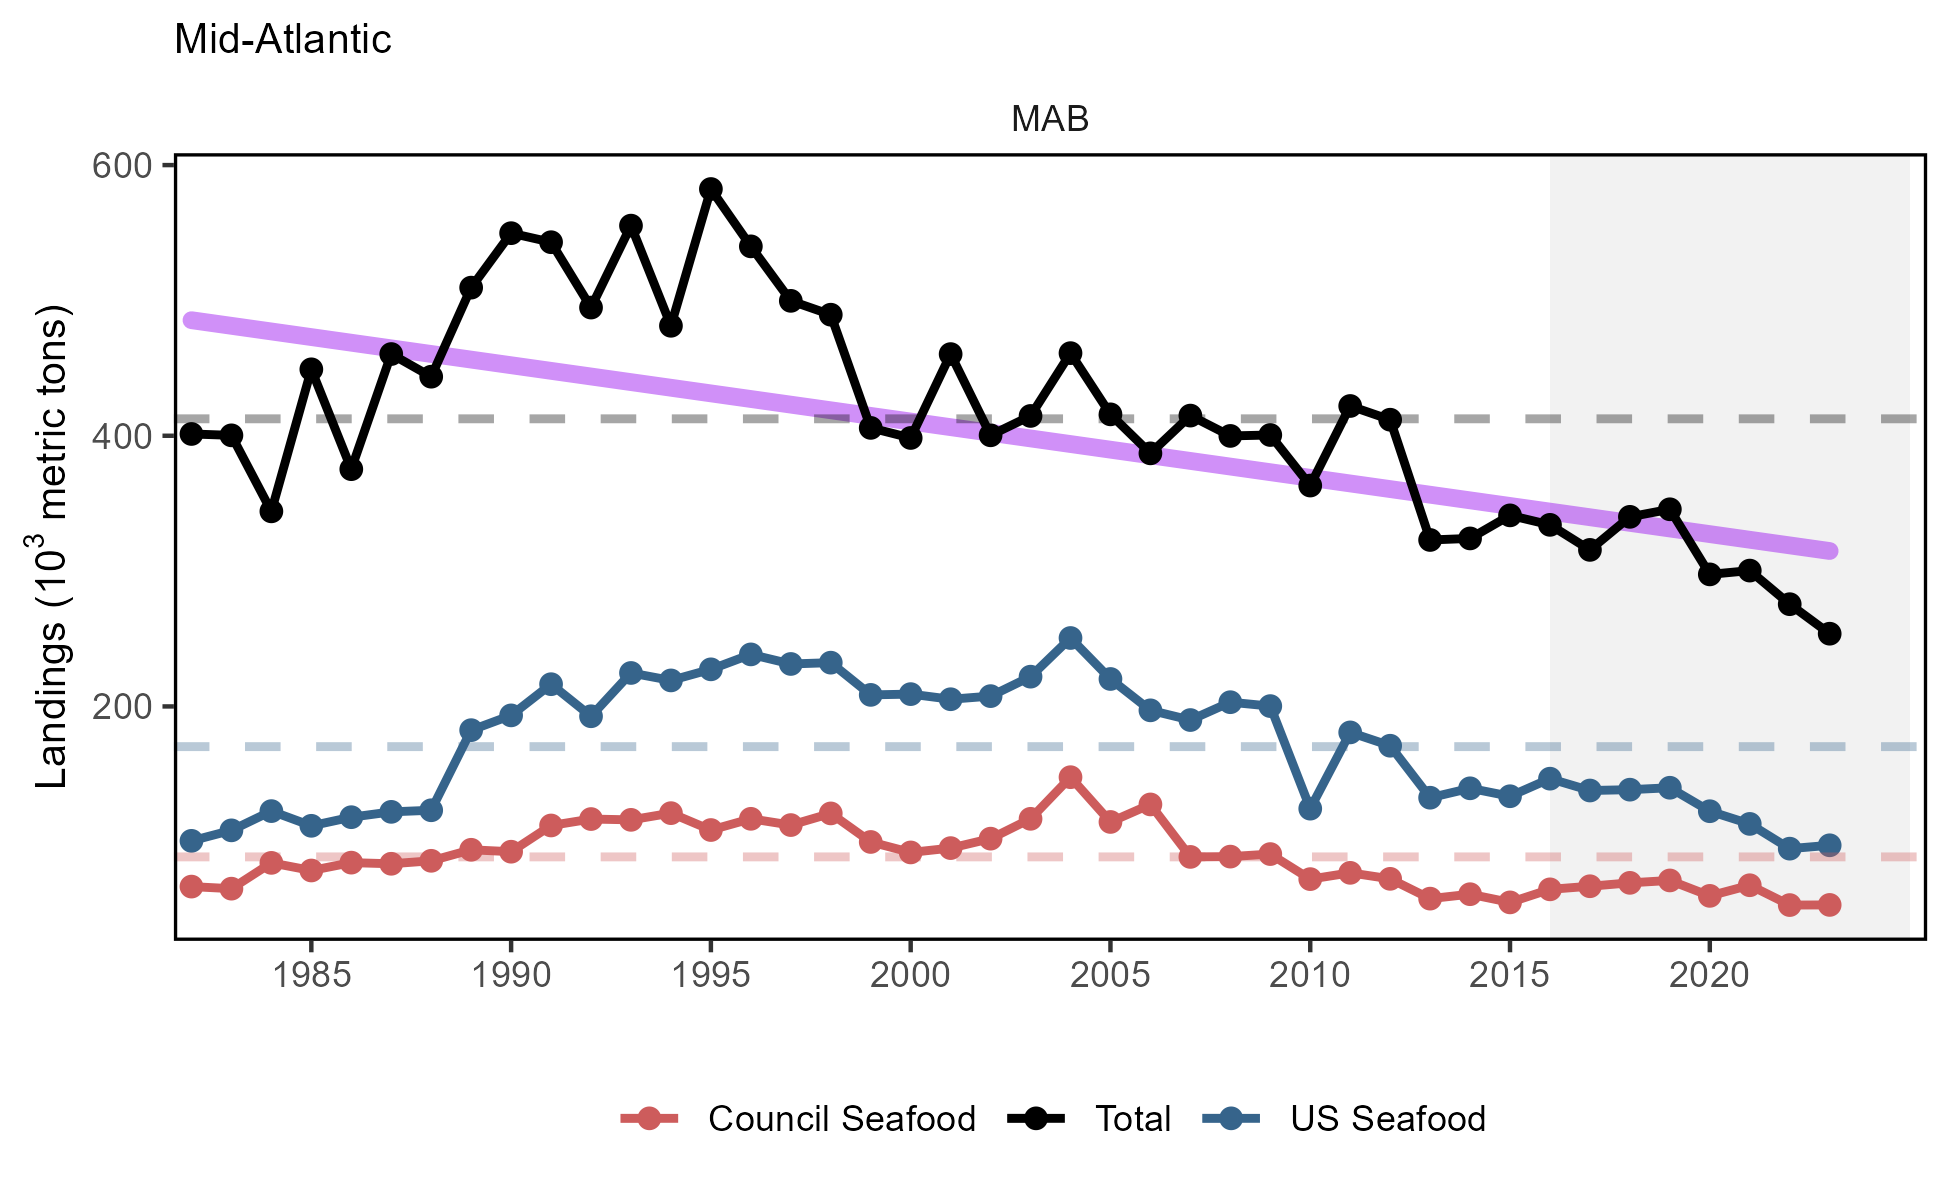
\includegraphics[width=6.5in]{images/MidAtlantic/total_landings_MidAtlantic_2025-09-05} 

}

\caption{Total commercial landings (black), total U.S. seafood landings (blue), and Mid-Atlantic managed U.S. seafood landings (red), with significant decline (purple) in total landings.}\label{fig:total-landings}
\end{figure}

Commercial landings by guild include all species and all uses, and are reported as total for the guild and the MAFMC managed species within the \href{https://noaa-edab.github.io/catalog/species_groupings.html}{guild}. Landings of benthos have been below the long term average since 2010, primarily driven by surf clam and ocean quahog, with scallops now contributing to the decline as well. Total landings of planktivores is presenting a significant downward trend, primarily due to decreases in species not managed by the MAFMC (Atlantic herring and Atlantic menhaden; Fig. \ref{fig:comm-landings}).

\begin{figure}

{\centering 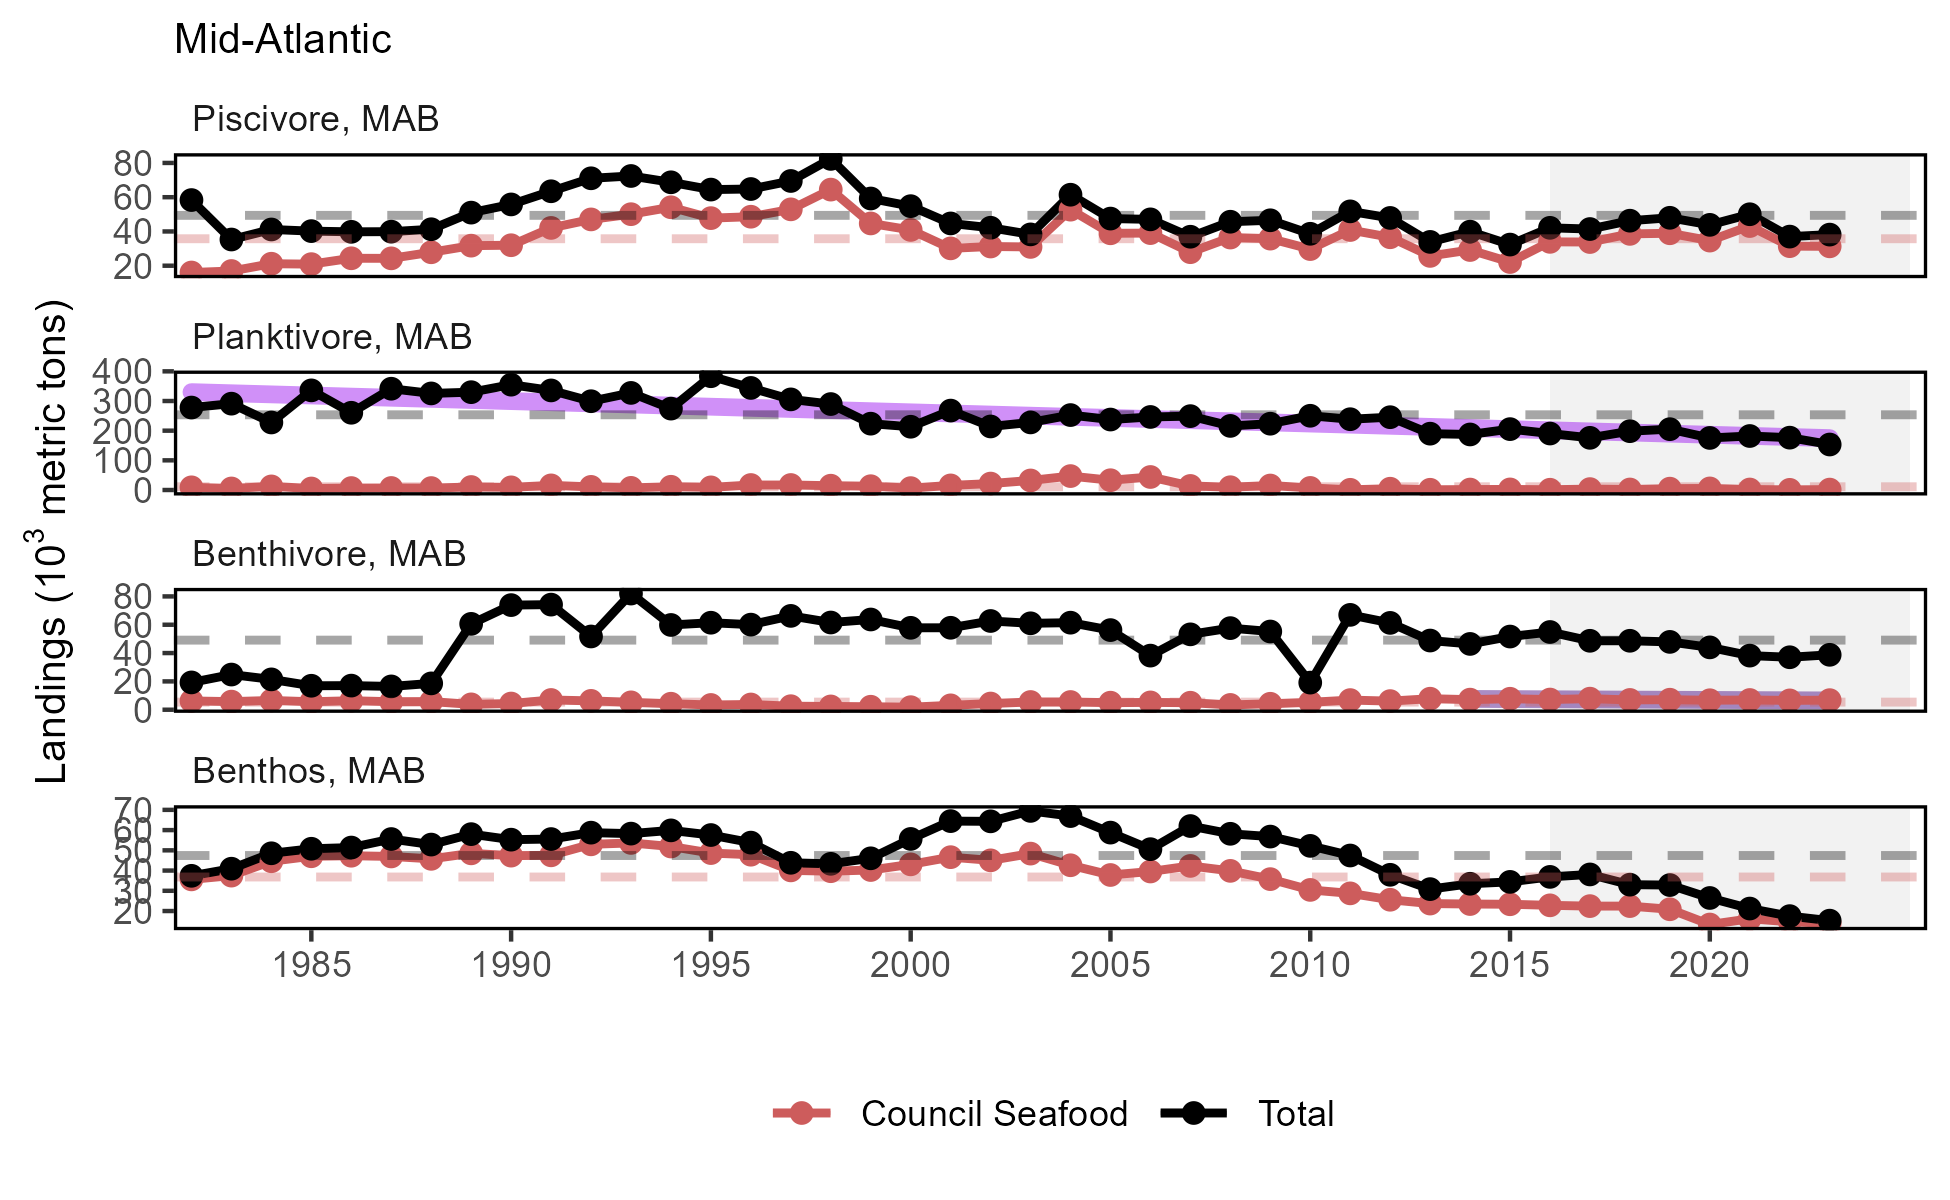
\includegraphics[width=6.5in]{images/MidAtlantic/commercial_landings_MidAtlantic_2025-09-05} 

}

\caption{Total commercial landings in the Mid-Atlantic Bight (black) and MAFMC-managed U.S seafood landings (red) by feeding guild, with significant declines (purple) in total planktivore landings.}\label{fig:comm-landings}
\end{figure}

\href{https://noaa-edab.github.io/catalog/community_climate_vulnerability.html}{Community Climate Change Risk indicators} have been developed to evaluate port specific landings and revenue risk in terms of commercial species climate vulnerability. The total climate vulnerability is a measure of to what degree a region's landings (or revenue) is dependent on species sensitive to different climate and environmental change factors including temperature and acidification. For ports combined across Mid-Atlantic states, the total climate vulnerability of landings ranged between moderate and high with a long term increase from 2000-2021 (Fig. \ref{fig:climatevul-land}).

\begin{figure}

{\centering 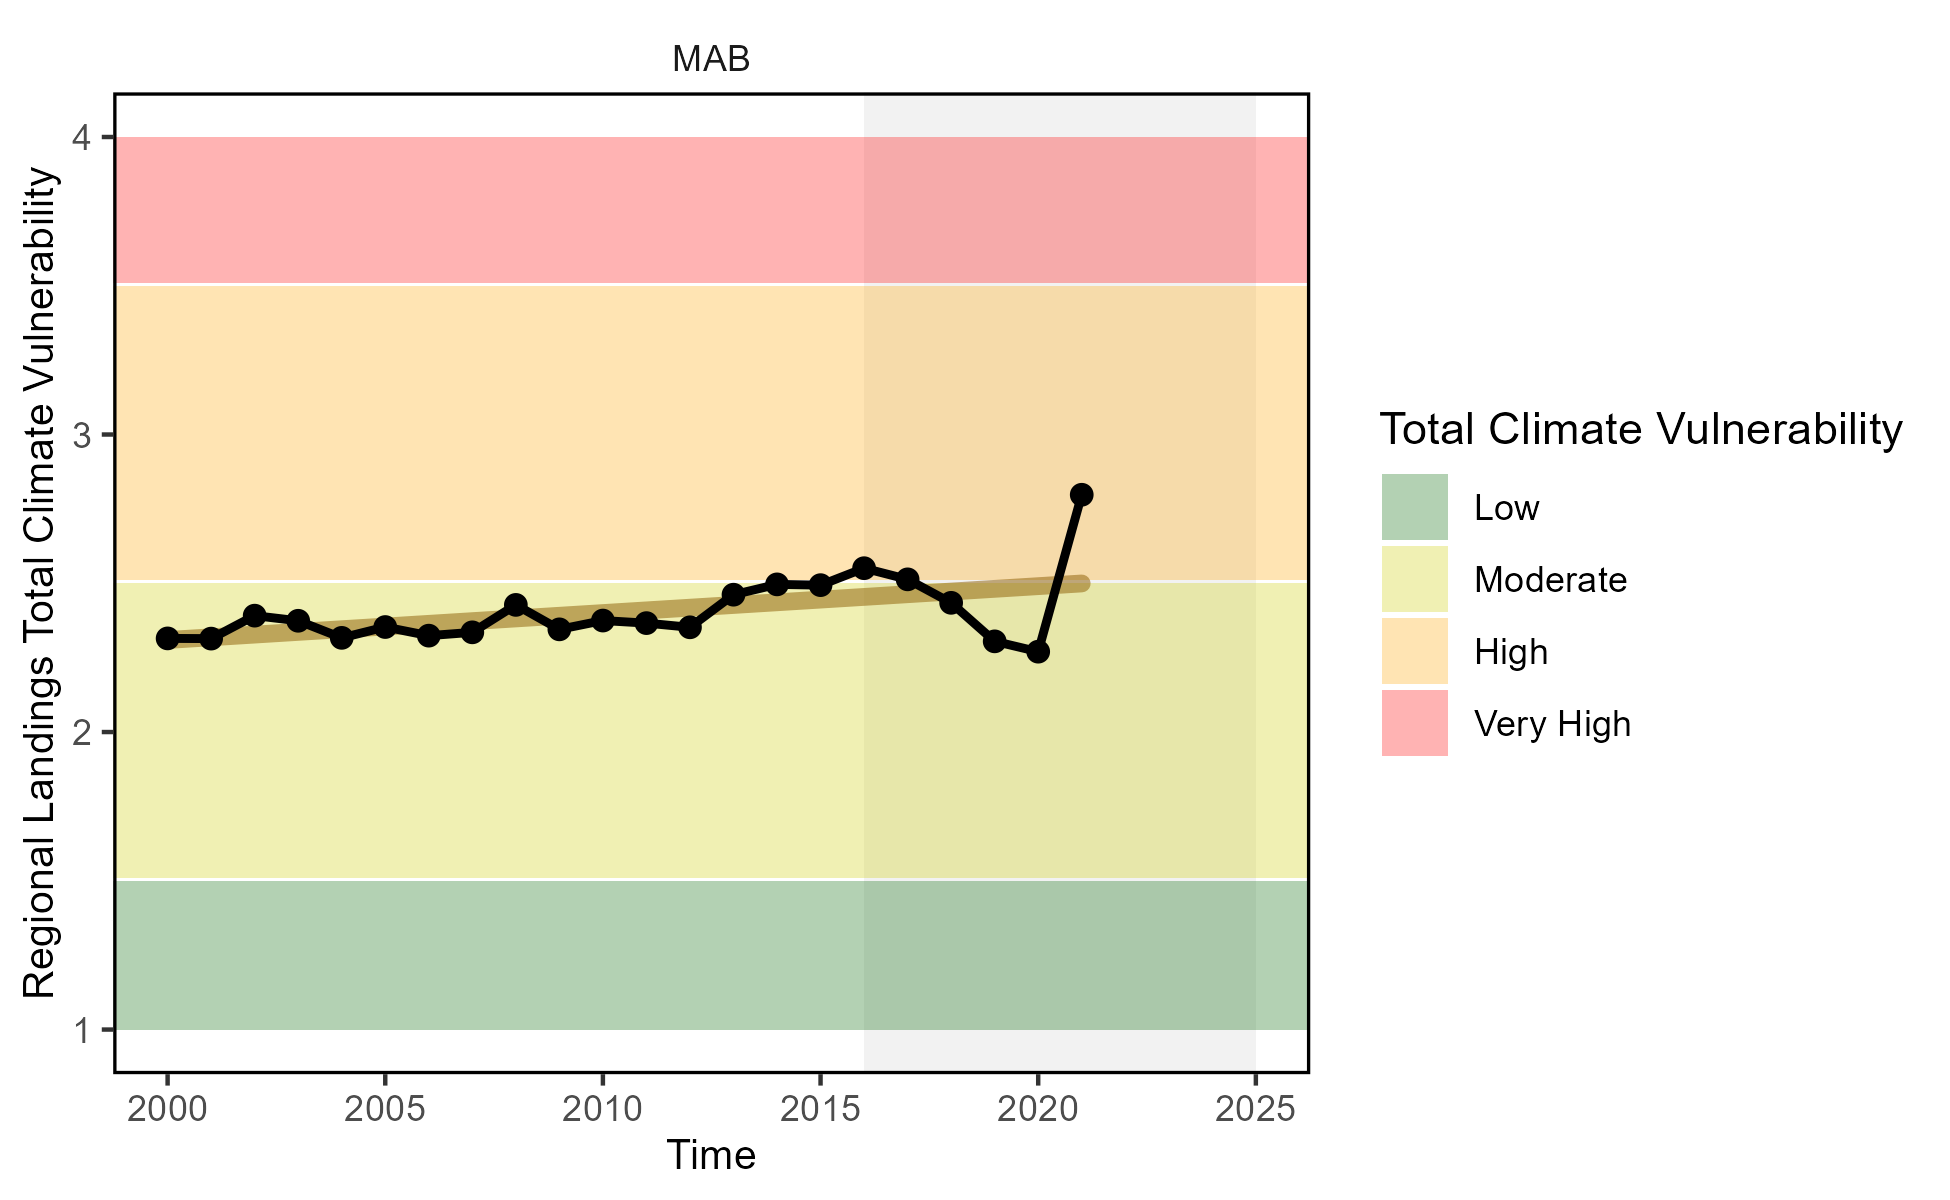
\includegraphics[width=6.5in]{images/MidAtlantic/climatevul_land_MidAtlantic_2025-09-05} 

}

\caption{Mid-Atlantic region total climate vulnerability of commercial landings (sum of Mid-Atlantic port landings weighted by species climate vulnerability from Hare et al. 2016).}\label{fig:climatevul-land}
\end{figure}

Although total \href{https://noaa-edab.github.io/catalog/recdat.html}{recreational harvest} (fish presumed to be eaten) has increased from a historic low in 2018, there is a long-term decline in the Mid-Atlantic (Fig. \ref{fig:rec-landings}).

\begin{figure}

{\centering 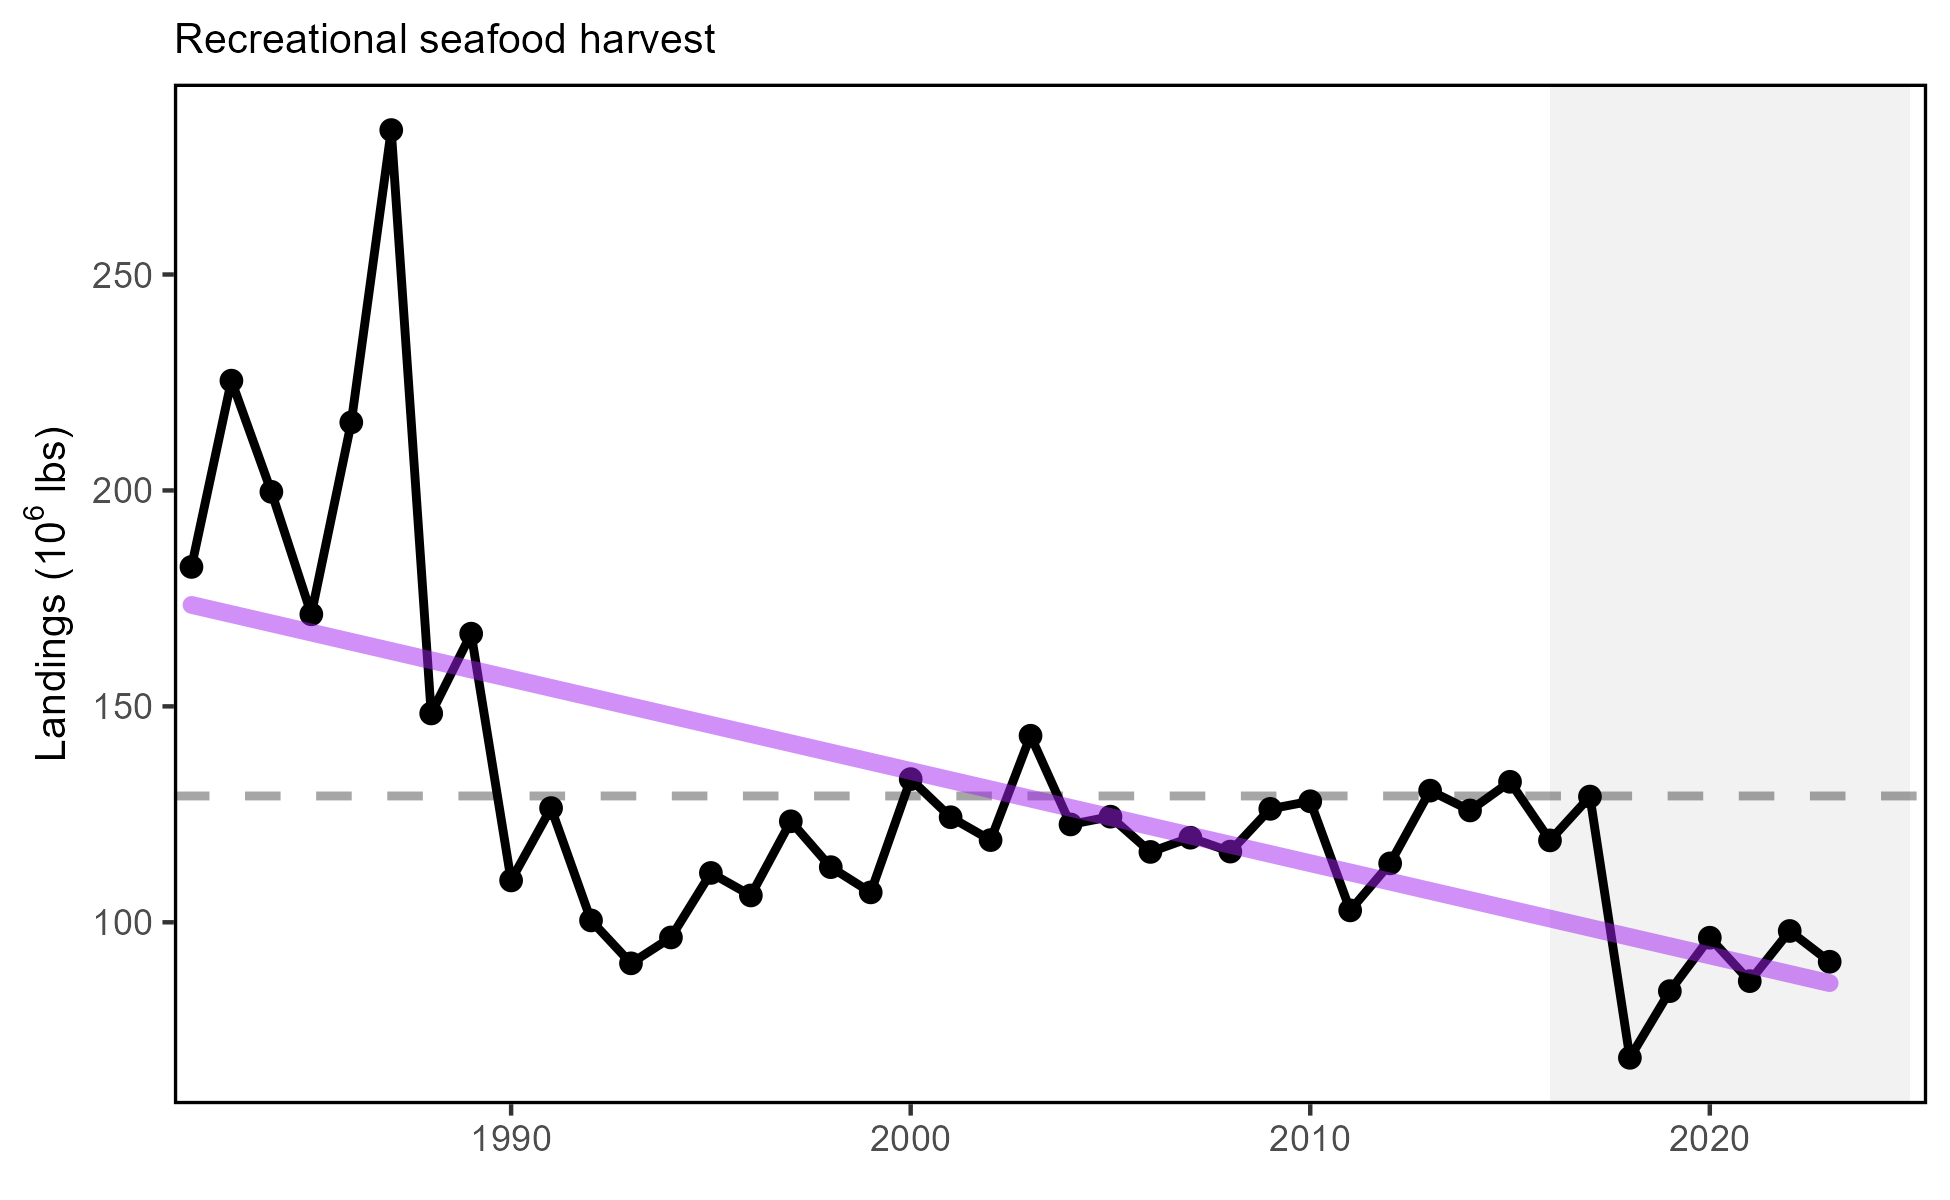
\includegraphics[width=6.5in]{images/MidAtlantic/rec_landings_MidAtlantic_2025-09-05} 

}

\caption{Total recreational seafood harvest (millions of pounds, black, significant decrease, purple) in the Mid-Atlantic region.}\label{fig:rec-landings}
\end{figure}

\href{https://noaa-edab.github.io/catalog/rec_hms.html}{Recreational shark landings} have generally decreased for most shark groups through 2023 (Fig \ref{fig:rec-hms}). The recent low in pelagic shark landings is likely influenced by regulatory changes implemented in 2018 intended to rebuild shortfin mako stocks and comply with binding recommendations by the International Commission for the Conservation of Atlantic Tunas (ICCAT).

\begin{figure}

{\centering 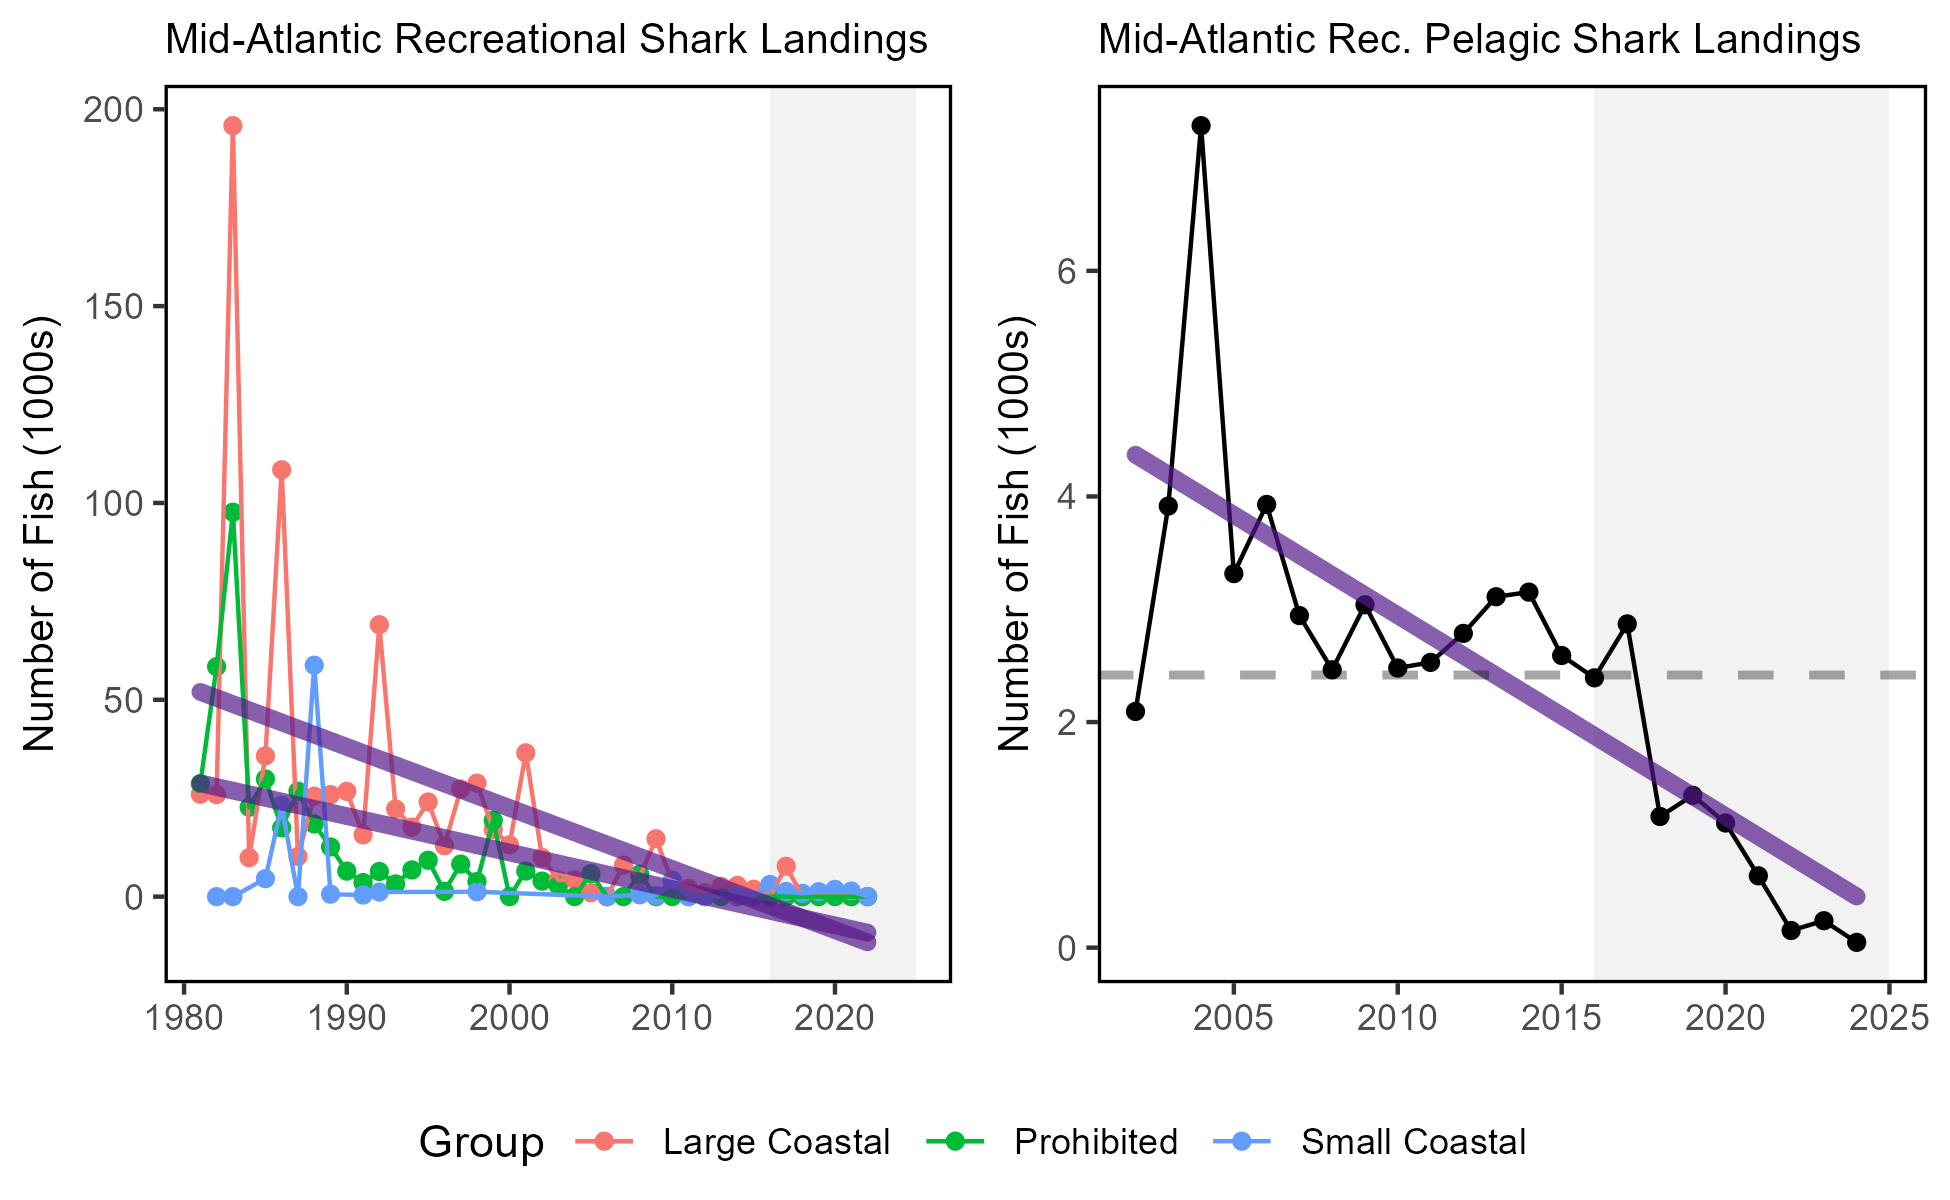
\includegraphics[width=6.5in]{images/MidAtlantic/rec_hms_MidAtlantic_2025-09-05} 

}

\caption{Recreational shark landings from Marine Recreational Information Program (left) and Large Pelagics Survey (right) with declining trends (purple).}\label{fig:rec-hms}
\end{figure}

Aquaculture production is not yet included in total seafood landings. Available \href{https://noaa-edab.github.io/catalog/aquaculture.html}{aquaculture production} of oysters for a subset of Mid-Atlantic states indicates a decline in recent years.

\subsubsection{Implications}\label{implications}

Declining commercial (total and seafood) landings and recreational harvest can be driven by many interacting factors, including combinations of ecosystem and stock production, management actions, market conditions, and environmental change. While we cannot evaluate all possible drivers at present, here we evaluate the extent to which stock status, management, and system biomass trends may play a role.

\paragraph{Stock Status and Catch Limits}\label{stock-status-and-catch-limits}

Single species \href{https://noaa-edab.github.io/catalog/stock_status.html}{management objectives} (1. maintaining biomass above minimum thresholds and 2. maintaining fishing mortality below overfishing limits) are being met for all but three MAFMC-managed species (Fig. \ref{fig:stock-status}), though the status of six stocks is unknown (Table \ref{tab:unkstocks}).

\begin{figure}

{\centering 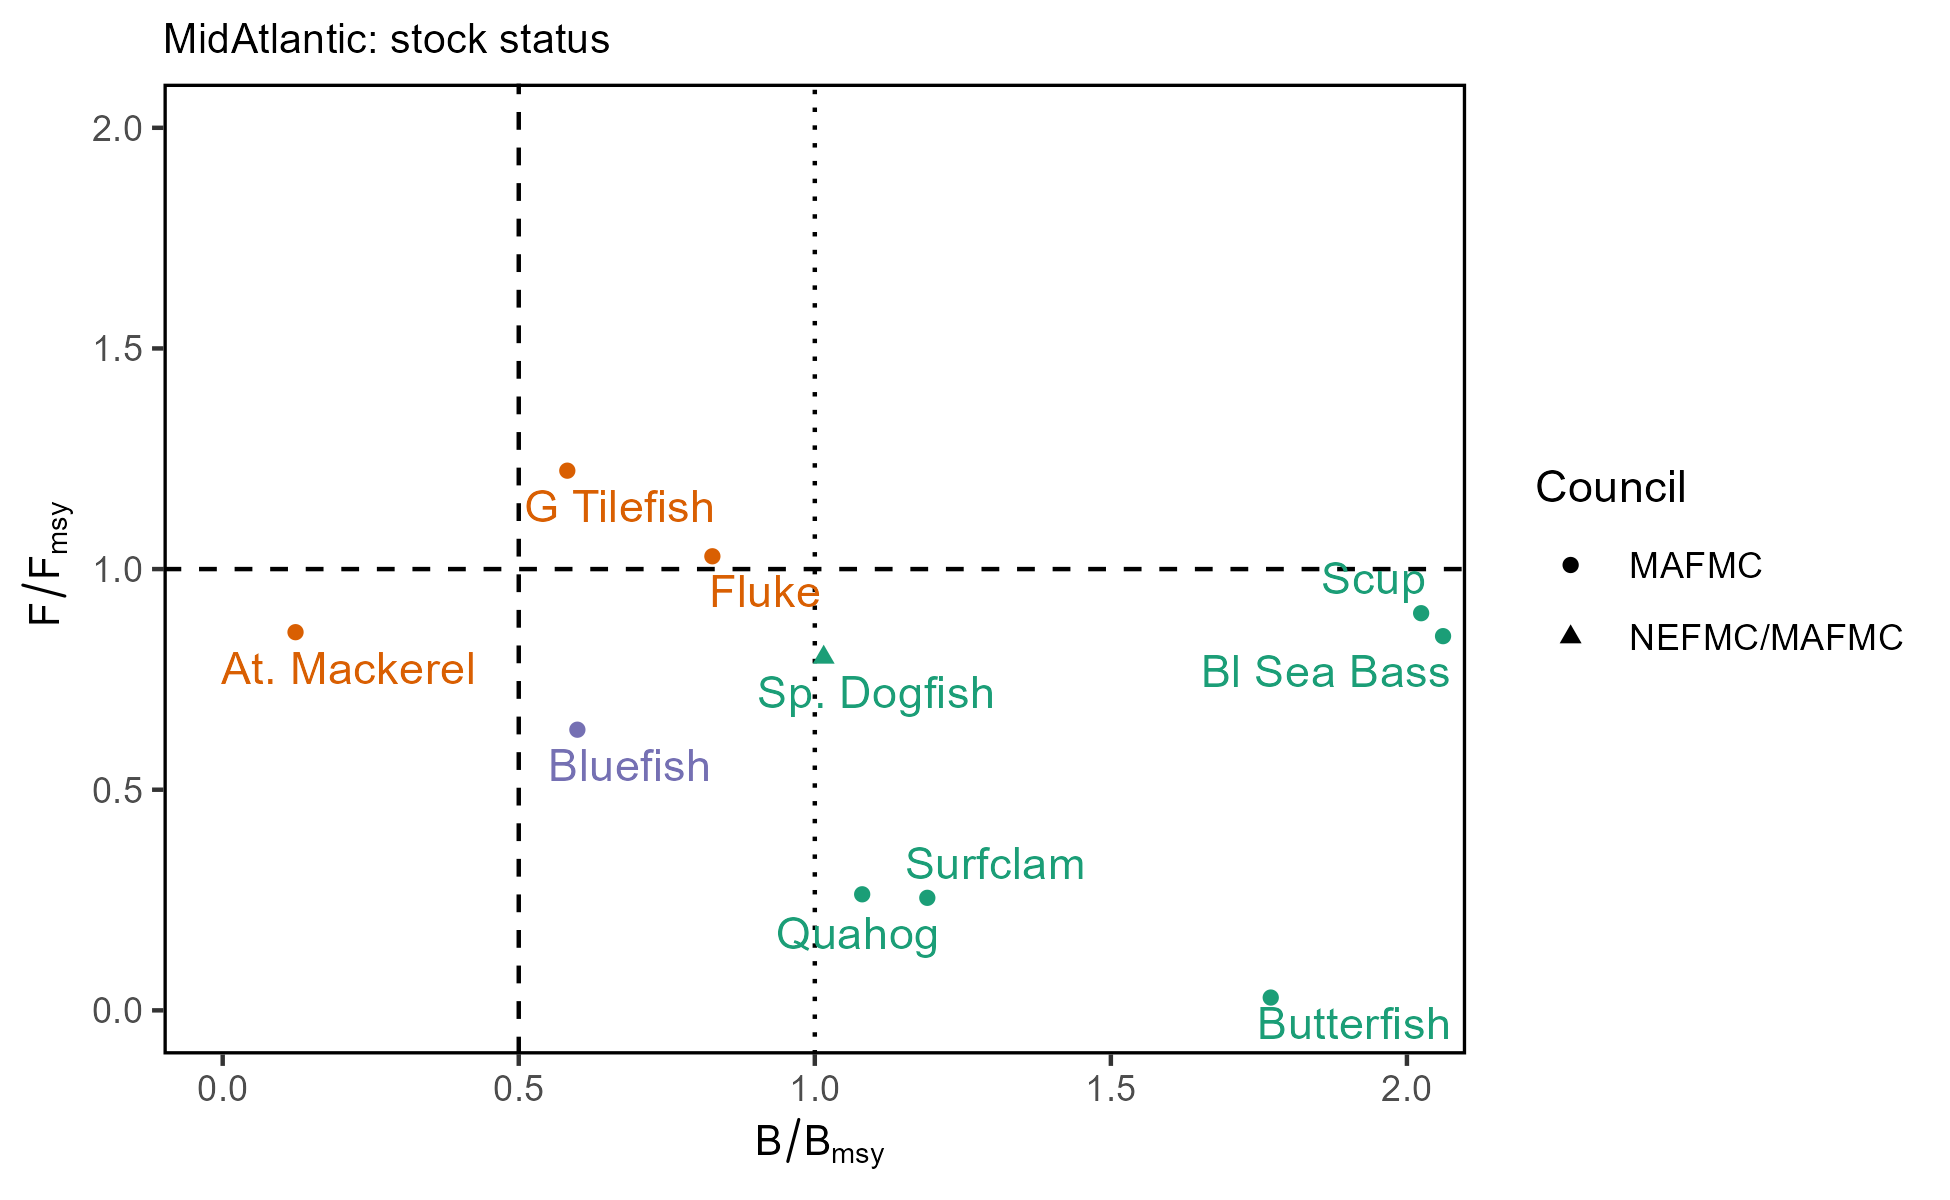
\includegraphics[width=6.5in]{images/MidAtlantic/stock_status_MidAtlantic_2025-09-05} 

}

\caption{Summary of single species status for MAFMC and jointly federally managed stocks (Spiny dogfish and both Goosefish). The dotted vertical line is the target biomass reference point of $B_{MSY}$. The dashed lines are the management thresholds of one half $B_{MSY}$ (vertical) or $F_{MSY}$. (horizontal). Stocks in orange are below the biomass threshold (overfished) or have fishing mortality above the limit (subject to overfishing), so are not meeting objectives. Stocks in purple  are above the biomass threshold but below the biomass target with fishing mortality within the limit. Stocks in green are above the biomass target, with fishing mortality within the limit.}\label{fig:stock-status}
\end{figure}

\global\setlength{\Oldarrayrulewidth}{\arrayrulewidth}

\global\setlength{\Oldtabcolsep}{\tabcolsep}

\setlength{\tabcolsep}{2pt}

\renewcommand*{\arraystretch}{1.5}



\providecommand{\ascline}[3]{\noalign{\global\arrayrulewidth #1}\arrayrulecolor[HTML]{#2}\cline{#3}}

\begin{longtable}[c]{|p{3.29in}|p{0.70in}|p{0.72in}}

\caption{Unknown\ or\ partially\ known\ stock\ status\ for\ MAFMC\ and\ jointly\ managed\ species.}\label{tab:unkstocks}\\

\ascline{1.5pt}{666666}{1-3}

\multicolumn{1}{>{\raggedright}m{\dimexpr 3.29in+0\tabcolsep}}{\textcolor[HTML]{000000}{\fontsize{9}{9}\selectfont{Stock}}} & \multicolumn{1}{>{\raggedleft}m{\dimexpr 0.7in+0\tabcolsep}}{\textcolor[HTML]{000000}{\fontsize{9}{9}\selectfont{F/Fmsy}}} & \multicolumn{1}{>{\raggedleft}m{\dimexpr 0.72in+0\tabcolsep}}{\textcolor[HTML]{000000}{\fontsize{9}{9}\selectfont{B/Bmsy}}} \\

\ascline{1.5pt}{666666}{1-3}\endfirsthead \caption[]{Unknown\ or\ partially\ known\ stock\ status\ for\ MAFMC\ and\ jointly\ managed\ species.}\label{tab:unkstocks}\\

\ascline{1.5pt}{666666}{1-3}

\multicolumn{1}{>{\raggedright}m{\dimexpr 3.29in+0\tabcolsep}}{\textcolor[HTML]{000000}{\fontsize{9}{9}\selectfont{Stock}}} & \multicolumn{1}{>{\raggedleft}m{\dimexpr 0.7in+0\tabcolsep}}{\textcolor[HTML]{000000}{\fontsize{9}{9}\selectfont{F/Fmsy}}} & \multicolumn{1}{>{\raggedleft}m{\dimexpr 0.72in+0\tabcolsep}}{\textcolor[HTML]{000000}{\fontsize{9}{9}\selectfont{B/Bmsy}}} \\

\ascline{1.5pt}{666666}{1-3}\endhead



\multicolumn{1}{>{\raggedright}m{\dimexpr 3.29in+0\tabcolsep}}{\textcolor[HTML]{000000}{\fontsize{9}{9}\selectfont{Longfin\ inshore\ squid\ -\ Georges\ Bank\ /\ Cape\ Hatteras}}} & \multicolumn{1}{>{\raggedleft}m{\dimexpr 0.7in+0\tabcolsep}}{\textcolor[HTML]{000000}{\fontsize{9}{9}\selectfont{-}}} & \multicolumn{1}{>{\raggedleft}m{\dimexpr 0.72in+0\tabcolsep}}{\textcolor[HTML]{000000}{\fontsize{9}{9}\selectfont{2.873}}} \\





\multicolumn{1}{>{\raggedright}m{\dimexpr 3.29in+0\tabcolsep}}{\textcolor[HTML]{000000}{\fontsize{9}{9}\selectfont{Northern\ shortfin\ squid\ -\ Northwestern\ Atlantic\ Coast}}} & \multicolumn{1}{>{\raggedleft}m{\dimexpr 0.7in+0\tabcolsep}}{\textcolor[HTML]{000000}{\fontsize{9}{9}\selectfont{-}}} & \multicolumn{1}{>{\raggedleft}m{\dimexpr 0.72in+0\tabcolsep}}{\textcolor[HTML]{000000}{\fontsize{9}{9}\selectfont{-}}} \\





\multicolumn{1}{>{\raggedright}m{\dimexpr 3.29in+0\tabcolsep}}{\textcolor[HTML]{000000}{\fontsize{9}{9}\selectfont{Goosefish\ -\ Gulf\ of\ Maine\ /\ Northern\ Georges\ Bank}}} & \multicolumn{1}{>{\raggedleft}m{\dimexpr 0.7in+0\tabcolsep}}{\textcolor[HTML]{000000}{\fontsize{9}{9}\selectfont{-}}} & \multicolumn{1}{>{\raggedleft}m{\dimexpr 0.72in+0\tabcolsep}}{\textcolor[HTML]{000000}{\fontsize{9}{9}\selectfont{-}}} \\





\multicolumn{1}{>{\raggedright}m{\dimexpr 3.29in+0\tabcolsep}}{\textcolor[HTML]{000000}{\fontsize{9}{9}\selectfont{Goosefish\ -\ Southern\ Georges\ Bank\ /\ Mid-Atlantic}}} & \multicolumn{1}{>{\raggedleft}m{\dimexpr 0.7in+0\tabcolsep}}{\textcolor[HTML]{000000}{\fontsize{9}{9}\selectfont{-}}} & \multicolumn{1}{>{\raggedleft}m{\dimexpr 0.72in+0\tabcolsep}}{\textcolor[HTML]{000000}{\fontsize{9}{9}\selectfont{-}}} \\





\multicolumn{1}{>{\raggedright}m{\dimexpr 3.29in+0\tabcolsep}}{\textcolor[HTML]{000000}{\fontsize{9}{9}\selectfont{Blueline\ tilefish\ -\ Mid-Atlantic\ Coast}}} & \multicolumn{1}{>{\raggedleft}m{\dimexpr 0.7in+0\tabcolsep}}{\textcolor[HTML]{000000}{\fontsize{9}{9}\selectfont{-}}} & \multicolumn{1}{>{\raggedleft}m{\dimexpr 0.72in+0\tabcolsep}}{\textcolor[HTML]{000000}{\fontsize{9}{9}\selectfont{-}}} \\





\multicolumn{1}{>{\raggedright}m{\dimexpr 3.29in+0\tabcolsep}}{\textcolor[HTML]{000000}{\fontsize{9}{9}\selectfont{Chub\ mackerel\ -\ Atlantic}}} & \multicolumn{1}{>{\raggedleft}m{\dimexpr 0.7in+0\tabcolsep}}{\textcolor[HTML]{000000}{\fontsize{9}{9}\selectfont{-}}} & \multicolumn{1}{>{\raggedleft}m{\dimexpr 0.72in+0\tabcolsep}}{\textcolor[HTML]{000000}{\fontsize{9}{9}\selectfont{-}}} \\

\ascline{1.5pt}{666666}{1-3}



\end{longtable}



\arrayrulecolor[HTML]{000000}

\global\setlength{\arrayrulewidth}{\Oldarrayrulewidth}

\global\setlength{\tabcolsep}{\Oldtabcolsep}

\renewcommand*{\arraystretch}{1}

Stock status affects catch limits established by the Council, which in turn may affect landings trends. Summed across all MAFMC managed species, total Acceptable Biological Catch or Annual Catch Limits \href{https://noaa-edab.github.io/catalog/abc_acl.html}{(ABC or ACL)} have been relatively stable 2012-2023 (Fig. \ref{fig:abcacl-stacked}). The recent total ABC or ACL is lower relative to 2012-2013, with much of that decrease due to declining Atlantic mackerel ABC. This is true even with the addition of blueline tilefish management contributing an additional ABC to the total post-2017, due to that fishery's small relative size.

\begin{figure}

{\centering 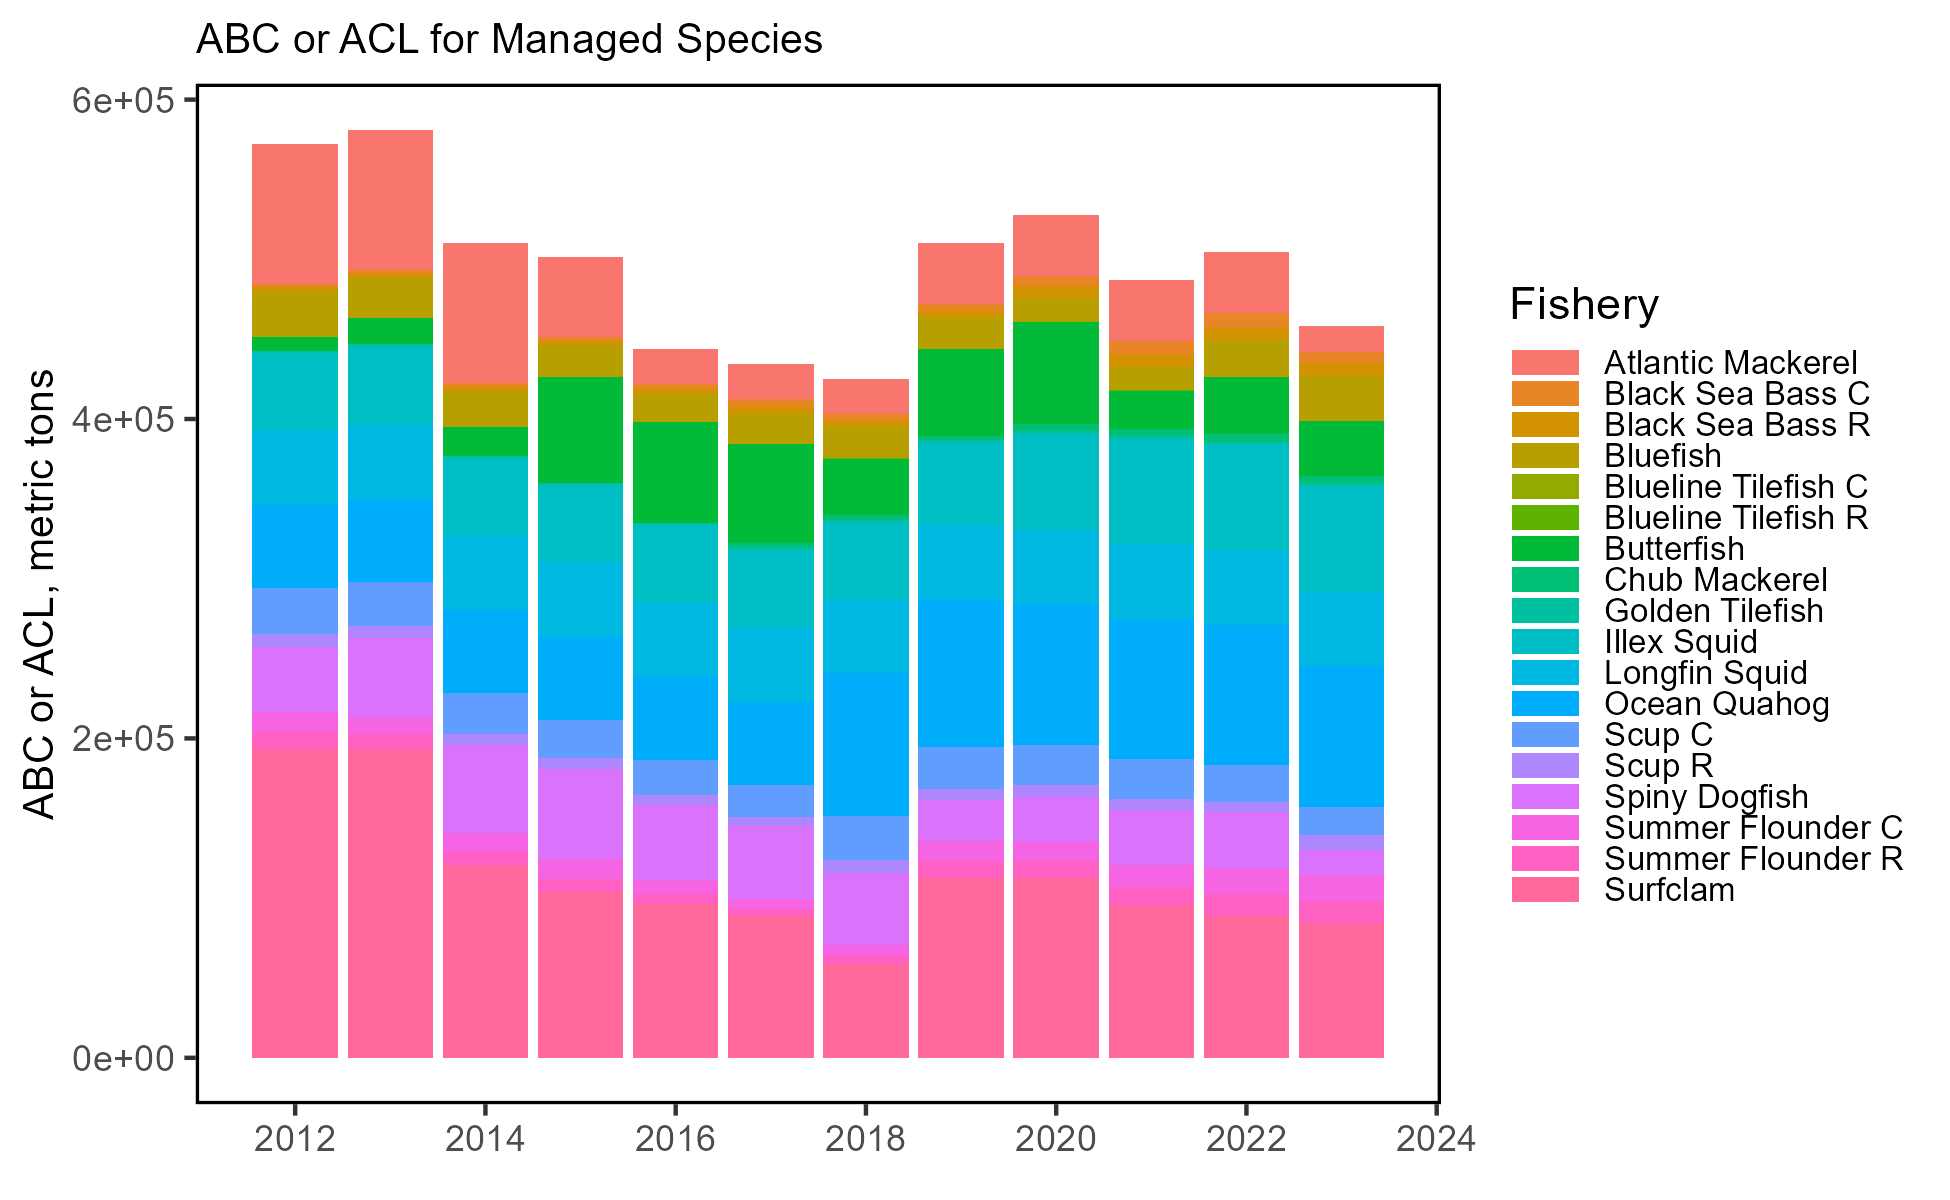
\includegraphics[width=6.5in]{images/MidAtlantic/abcacl_stacked_MidAtlantic_2025-09-05} 

}

\caption{Sum of catch limits across all MAFMC managed commercial (C) and recreational (R) fisheries.}\label{fig:abcacl-stacked}
\end{figure}

Nevertheless, the percentage caught (landings and discards) for each stock's ABC/ACL suggests that these catch limits are not generally constraining as most species are well below the 1/1 ratio (Fig. \ref{fig:abcacl-catch}). Therefore, stock status and associated management constraints are unlikely to be driving decreased landings for the majority of species.

\begin{figure}

{\centering 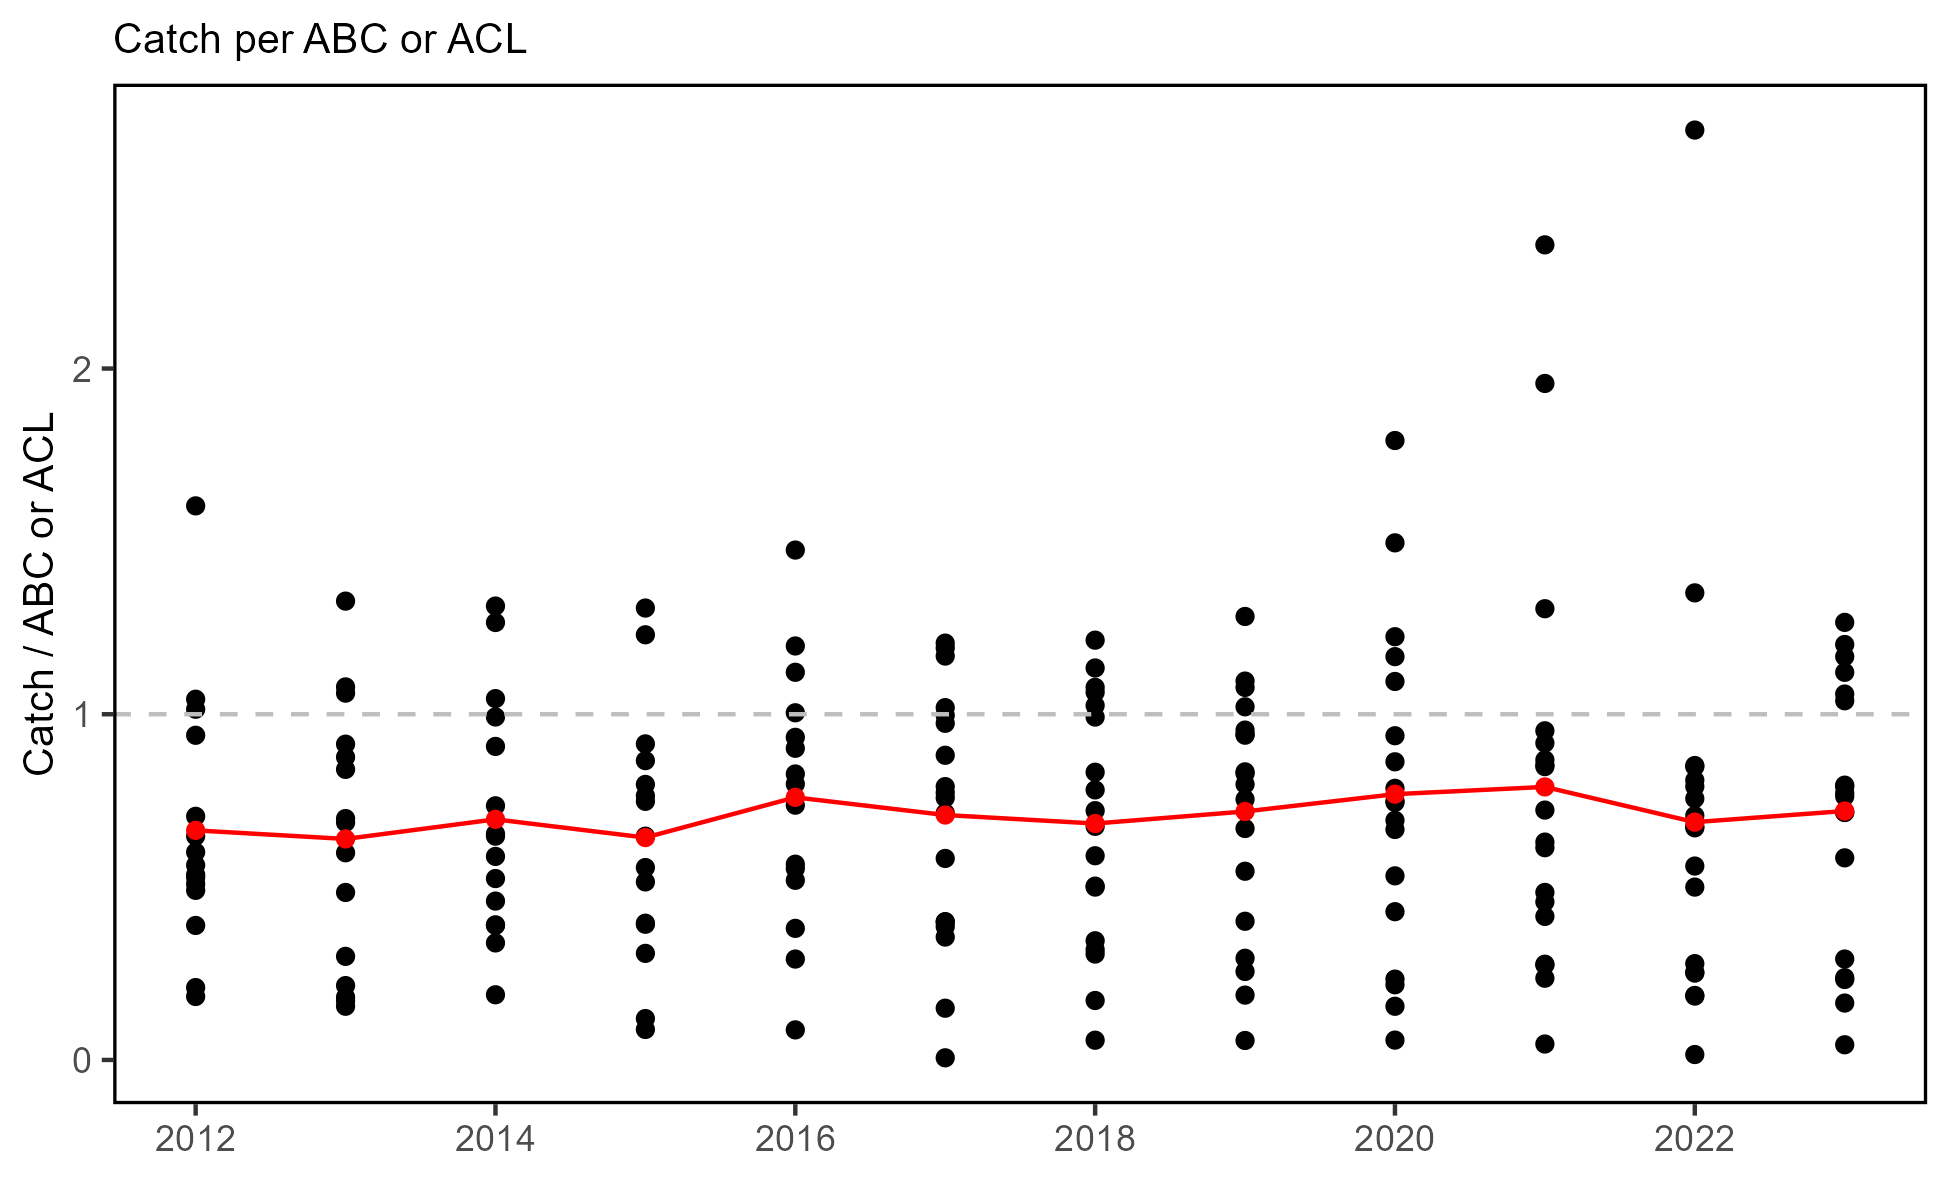
\includegraphics[width=6.5in]{images/MidAtlantic/abcacl_catch_MidAtlantic_2025-09-05} 

}

\caption{Catch divided by ABC/ACL for MAFMC managed fisheries. High points are recreational black sea bass (up to 2021) and scup (2022). Red line indicates the median ratio across all fisheries.}\label{fig:abcacl-catch}
\end{figure}

\paragraph{System Biomass}\label{system-biomass}

Although \href{https://noaa-edab.github.io/catalog/aggregate_biomass.html}{aggregate biomass} trends derived from scientific resource surveys are mostly stable in the MAB, spring piscivores, fall benthivores, and fall benthos show long-term increases (Fig. \ref{fig:nefsc-biomass-mab}). While managed species make up varying proportions of aggregate biomass, trends in landings are not mirroring shifts in the overall trophic structure of survey-sampled fish and invertebrates. Therefore, major shifts in feeding guilds or ecosystem trophic structure are unlikely to be driving the decline in landings.

\paragraph{Effect on Seafood Production}\label{effect-on-seafood-production}

Stock status is above the minimum threshold for all but one stock, and aggregate biomass trends appear stable or increasing, so the decline in managed commercial seafood landings is most likely driven by market dynamics affecting the landings of surfclams and ocean quahogs, as landings have been below quotas for these species. In addition, regional availability of scallops has contributed to the decline of benthos landings not managed by the MAFMC, with some of the most productive grounds closed through 2023 due to rotational management. The long term decline in total planktivore landings, and total landings, is largely driven by Atlantic menhaden fishery dynamics, including a consolidation of processors leading to reduced fishing capacity between the 1990s and mid-2000s.

The distribution of surfclams and ocean quahogs is changing, resulting in areas with overlapping distributions and increased mixed landings. Given the regulations governing mixed landings, this could have become problematic and the Council recently took final action to address this issue.

The decline in recreational seafood harvest stems from other drivers. Some of the decline, such as that for recreational shark landings, is driven by management intended to reduce fishing mortality on mako sharks. However, NOAA Fisheries' Marine Recreational Information Program survey methodology was updated in 2018, so it is unclear whether the lower than average landings for species other than sharks since 2018 are driven by changes in fishing behavior or the change in the survey methodology. Nevertheless, the recreational harvest appears to be stabilizing at a lower level than historical estimates.

Other environmental changes require monitoring as they may become important drivers of commercial and recreational landings in the future. Overall, landings from Mid-Atlantic ports depend on species with moderate climate vulnerability, and the proportion of landings with higher vulnerability has increased over time. We note that individual stocks will respond differently to these drivers, and fisheries and communities rely on different combinations of stocks:

\begin{itemize}
\tightlist
\item
  Climate is trending into uncharted territory. Globally, 2024 was the warmest year on record (see \hyperref[highlights]{2024 Highlights section}).
\item
  Stocks are shifting their distributions, moving towards the northeast and into deeper waters throughout the Northeast US Large Marine Ecosystem (see \hyperref[climate-and-ecosystem-change]{Climate Risks section}).
\item
  Some ecosystem composition and production changes have been observed (see \hyperref[stability]{Stability section}).
\item
  Some fishing communities are affected by socioeconomic vulnerabilities (see \hyperref[community-social-and-climate-vulnerability]{Community Social and Climate Vulnerability section}).
\end{itemize}

\section{parent\_report.Rmd}\label{parent_report.rmd-1}

\section{01\_seafood\_production\_newengland.Rmd}\label{seafood_production_newengland.rmd}

\subsubsection{Indicators: Landings; commercial and recreational}\label{indicators-landings-commercial-and-recreational-1}

This year, we present updated indicators for total \href{https://noaa-edab.github.io/catalog/comdat.html}{commercial landings}, U.S. seafood landings (includes seafood, bait, and industrial landings), and Council-managed U.S. seafood landings through 2023. There are long-term declines in all New England landings time series except for total commercial landings on GB (Fig. \ref{fig:total-landings}). There exist long-term declines in commercial seafood landings and NEFMC managed seafood landings for both the GOM and GB, but over the last decade there is no trend in managed seafood landings in the GOM.

\begin{figure}

{\centering 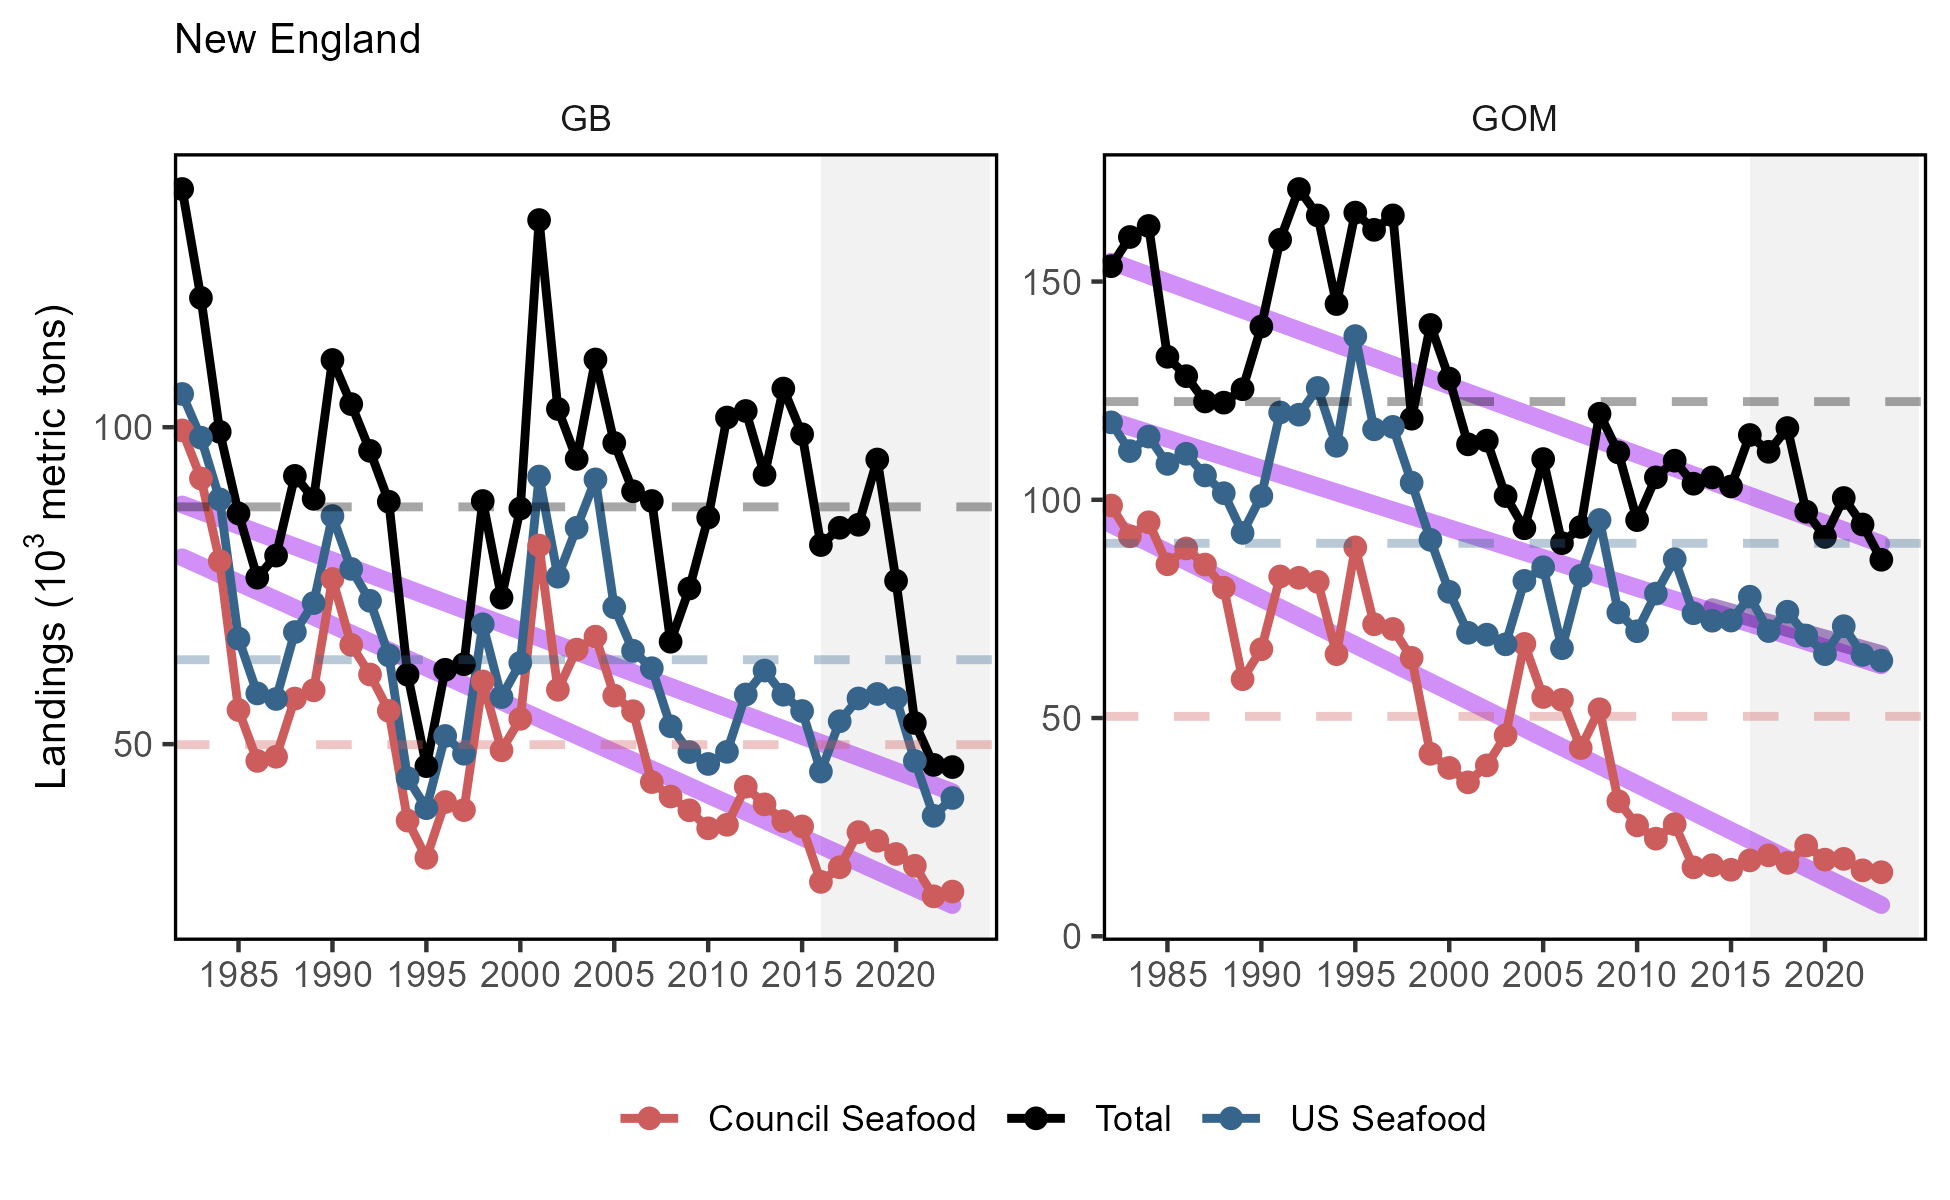
\includegraphics[width=6.5in]{images/NewEngland/total_landings_NewEngland_2025-09-09} 

}

\caption{Total commercial landings (black), total U.S. seafood landings (blue), and New England managed U.S. seafood landings (red) for Georges Bank (GB) and the Gulf of Maine (GOM).}\label{fig:total-landings-46}
\end{figure}

Commercial landings by guild include all species and all uses, and are reported as total for the guild and the NEFMC managed species within the \href{https://noaa-edab.github.io/catalog/aggregate_biomass.html}{guild}. As reported in previous years, downward trends persist for a number of guilds in both regions. Current high total landings for benthivores (GOM) are attributable to American lobster, and a significant long term increase in benthos landings (GB) is attributable to clams and scallops (Fig. \ref{fig:comm-landings}).Current landings of planktivores are still below the long term mean.

\href{https://noaa-edab.github.io/catalog/aquaculture.html}{Aquaculture production} is not yet included in total seafood landings.

\begin{figure}

{\centering 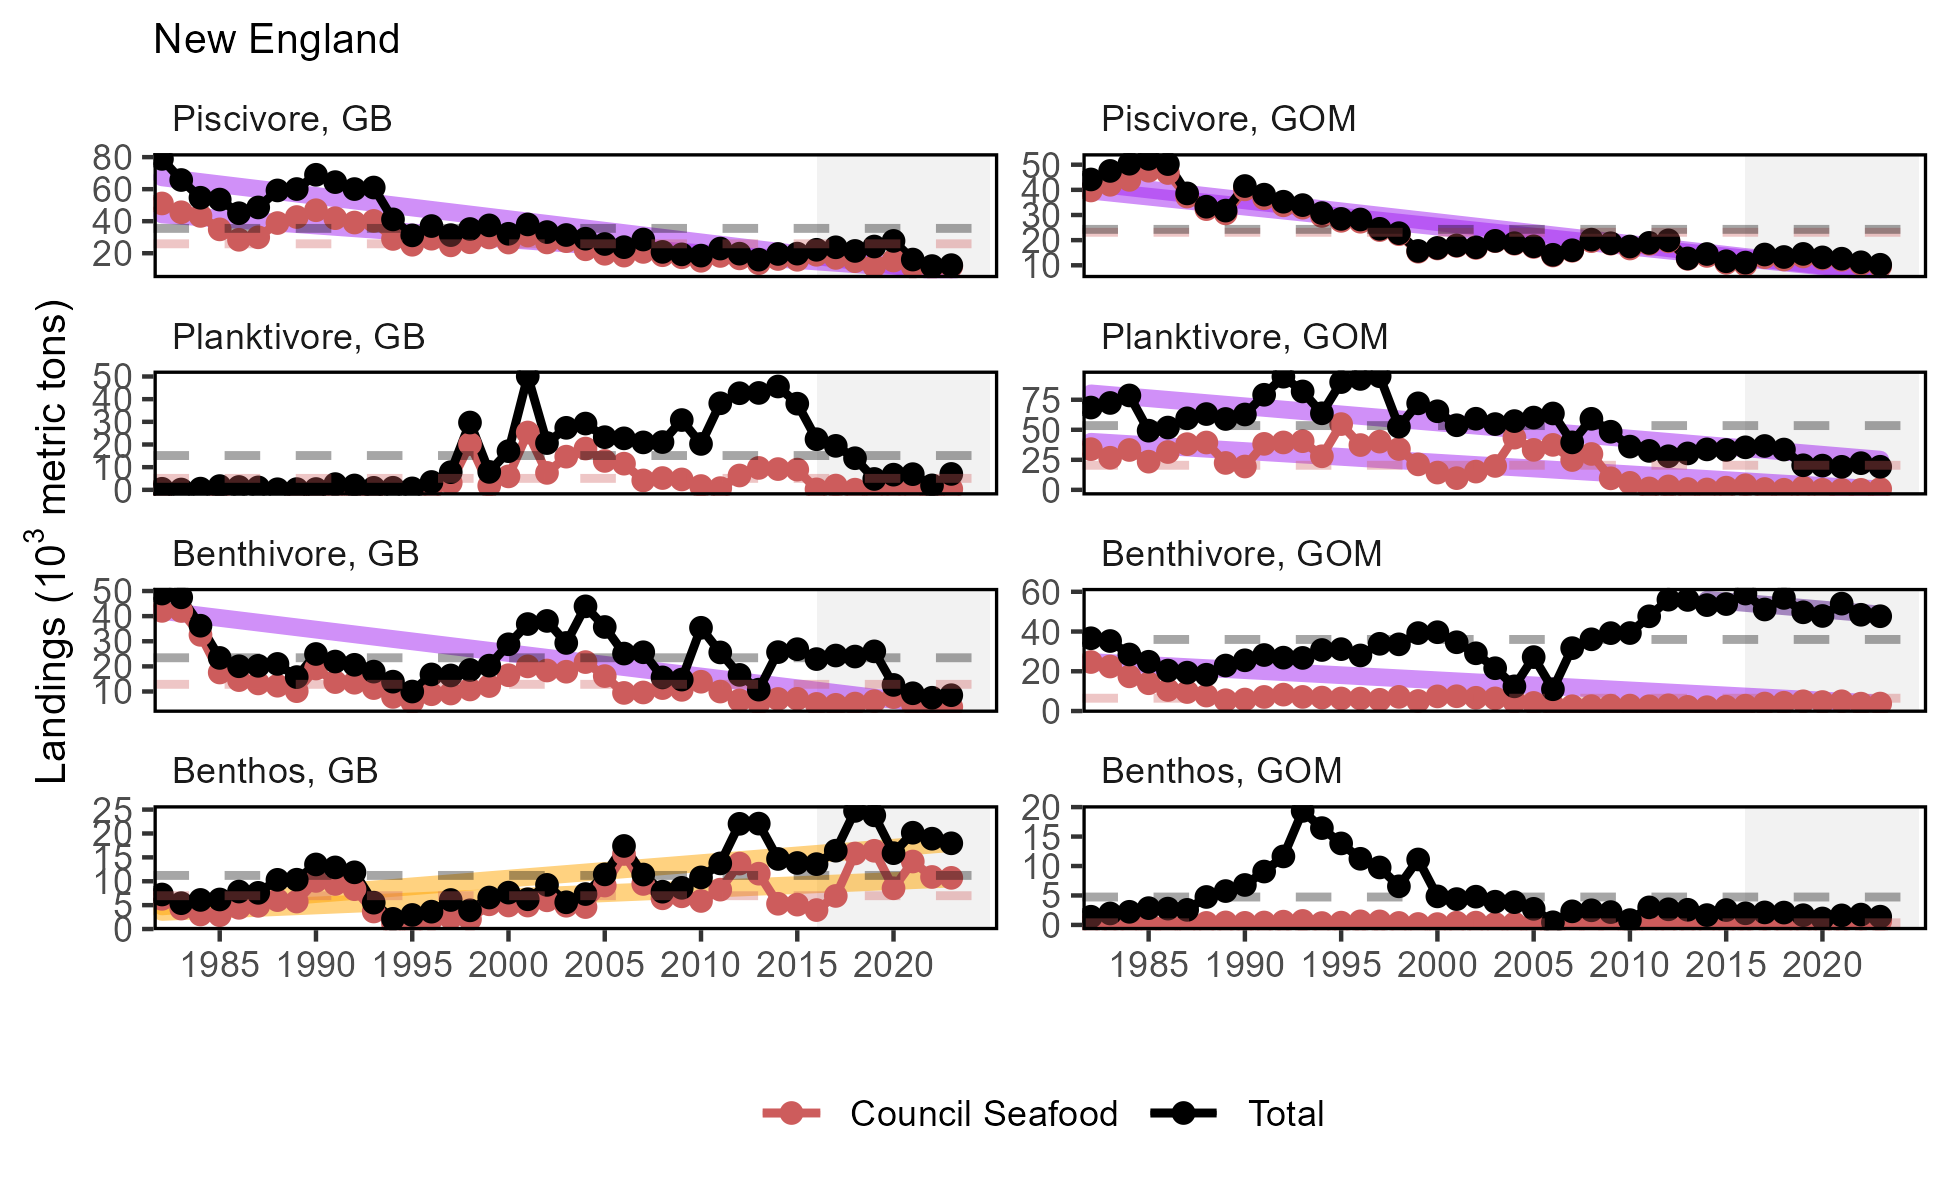
\includegraphics[width=6.5in]{images/NewEngland/commercial_landings_NewEngland_2025-09-09} 

}

\caption{Total commercial landings (black) and NEFMC managed U.S seafood landings (red) by feeding guild for the Gulf of Maine (GOM, right) and Georges Bank (GB, left).}\label{fig:comm-landings-47}
\end{figure}

\href{https://noaa-edab.github.io/catalog/community_climate_vulnerability.html}{Total Community Climate Change Risk} is a measure of to what degree a region's landings (or revenue) is dependent on sensitivity and exposure factors that relate to species' risk to temperature or ocean acidification changes as the result of future climate change. For New England, the total climate vulnerability of landings (Fig. \ref{fig:climatevul-land}) was moderate in 2022 with no long-term trend suggesting a moderate reliance on climate-sensitive species. This proportion has not significantly changed since 2000.

\begin{figure}

{\centering 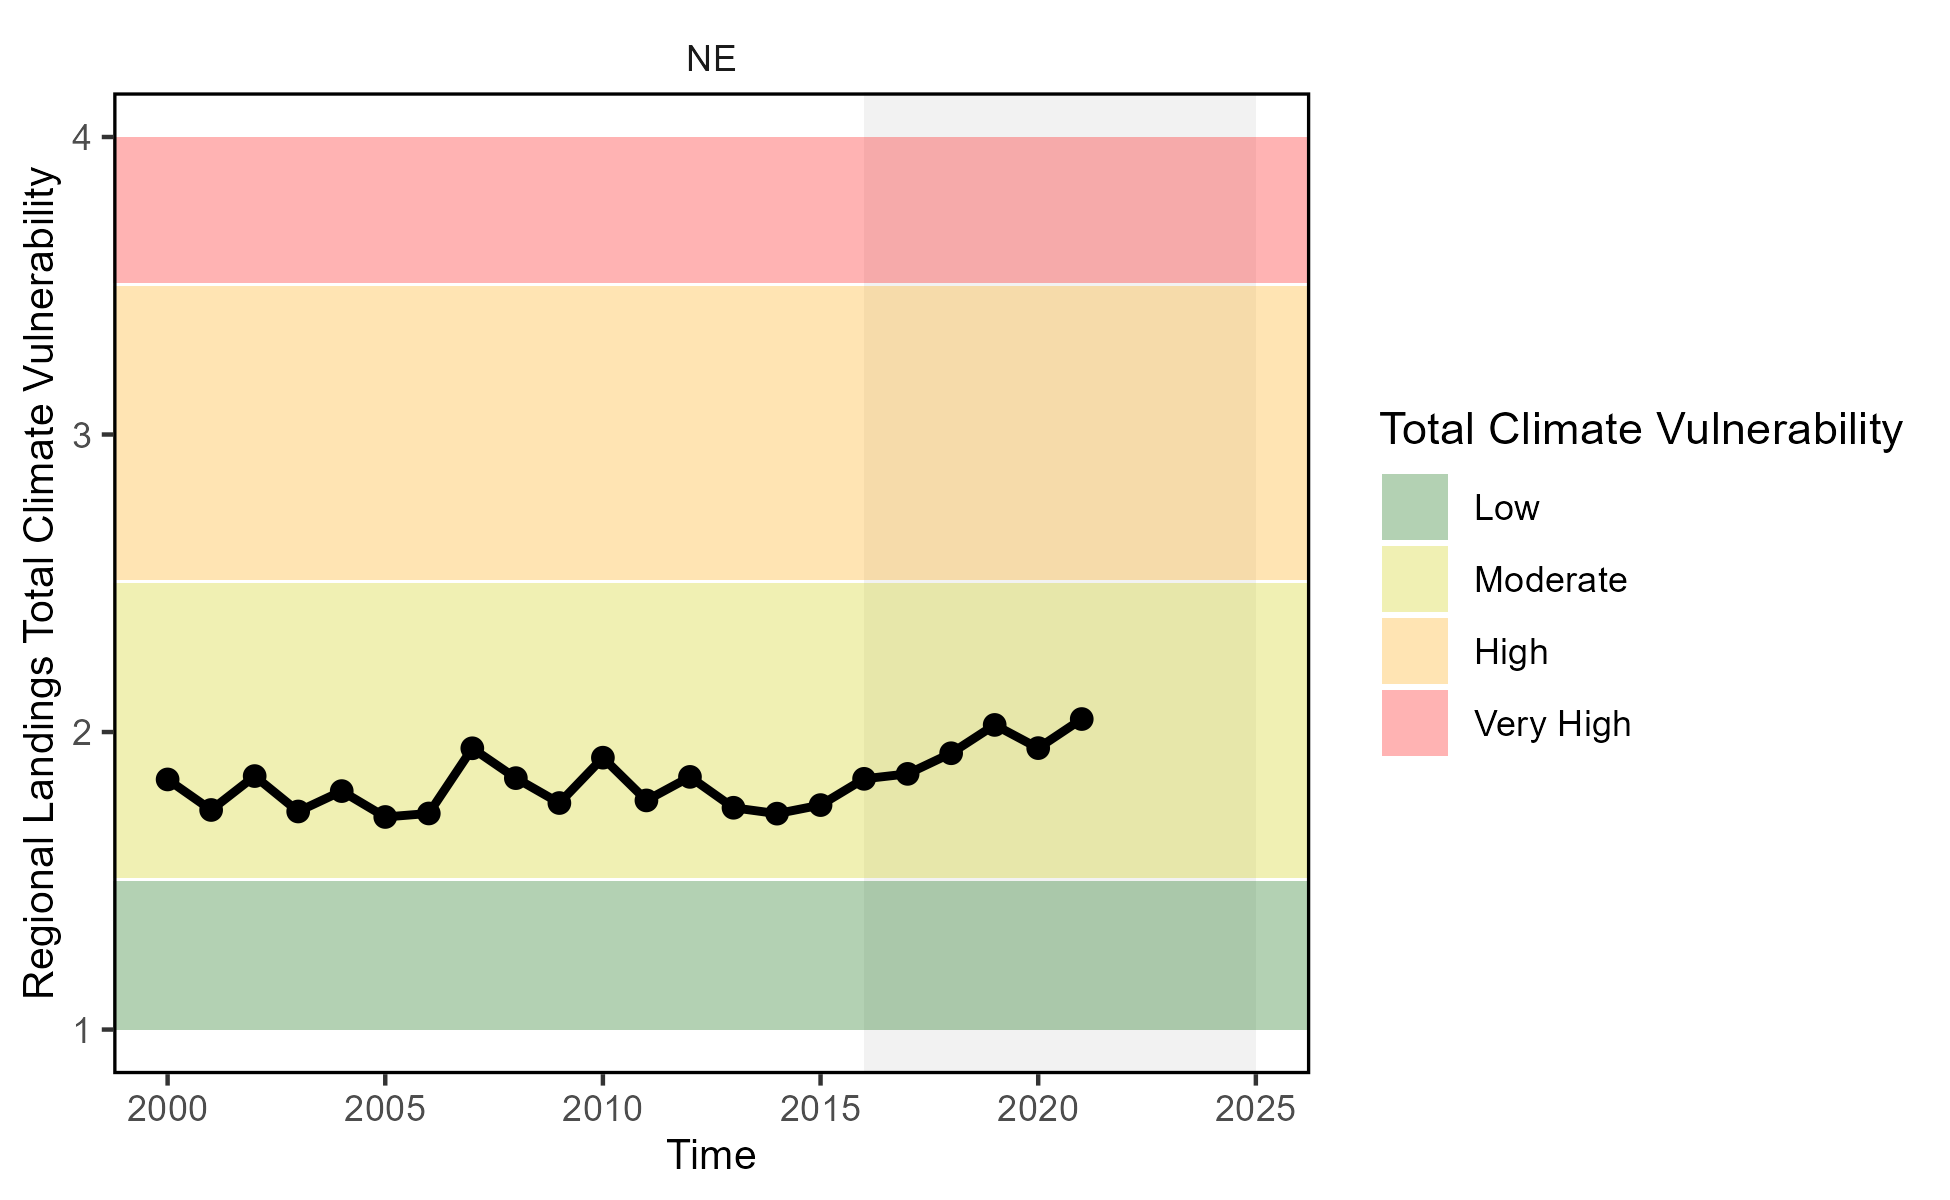
\includegraphics[width=6.5in]{images/NewEngland/climatevul_land_NewEngland_2025-09-09} 

}

\caption{Total climate vulnerability on New England landings from 2000 to 2022. Horizontal colored bars show different climate risk levels.}\label{fig:climatevul-land-48}
\end{figure}

Overall, \href{https://noaa-edab.github.io/catalog/recdat.html}{recreational harvest} (retained fish presumed to be eaten) has declined in New England (Fig. \ref{fig:rec-landings}). However, recent harvest has remained above the historical low level in 2020. Recreational \href{https://noaa-edab.github.io/catalog/rec_hms.html}{shark landings} of pelagic and prohibited sharks have declined since 2018 (Fig \ref{fig:rec-hms}), which is likely influenced by regulatory changes implemented in 2018 intended to rebuild shortfin mako stocks and comply with binding recommendations by the International Commission for the Conservation of Atlantic Tunas (ICCAT).

\begin{figure}

{\centering 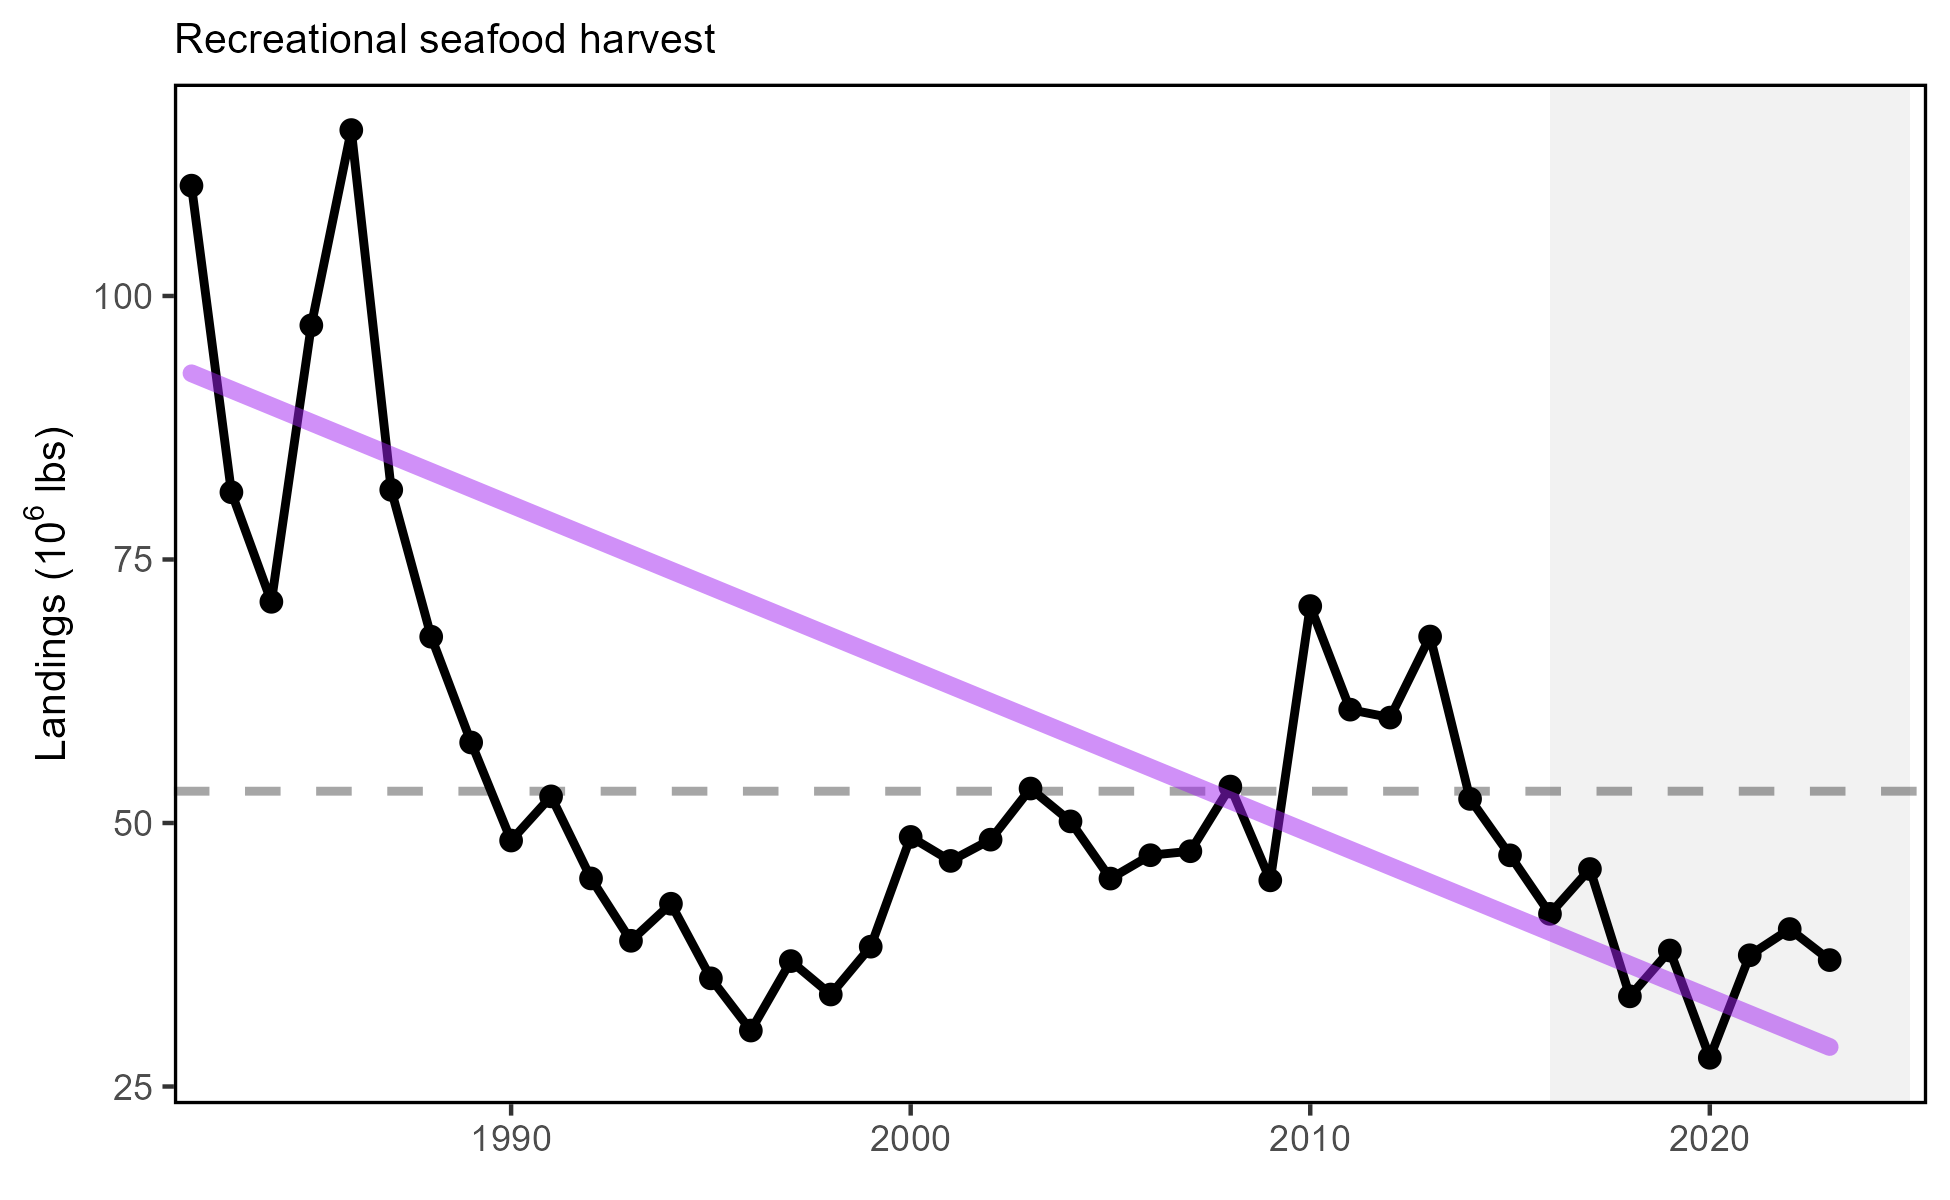
\includegraphics[width=6.5in]{images/NewEngland/rec_landings_NewEngland_2025-09-09} 

}

\caption{Total recreational seafood harvest (millions of pounds) in the New England region.}\label{fig:rec-landings-49}
\end{figure}

\subsubsection{Implications}\label{implications-1}

Declining commercial (total and seafood) landings and recreational harvest can be driven by many interacting factors, including combinations of ecosystem and stock production, management actions, market conditions, and environmental change. While we cannot evaluate all possible drivers at present, here we evaluate the extent to which stock status, management, and system biomass trends may play a role.

\paragraph{Stock Status}\label{stock-status}

Single species \href{https://noaa-edab.github.io/catalog/stock_status.html}{management objectives} (1. maintaining biomass above minimum thresholds and 2. maintaining fishing mortality below overfishing limits) are not being met for some NEFMC managed species. Thirteen stocks are currently estimated to be below B\textsubscript{MSY} (Fig. \ref{fig:stock-status}), while status relative to B\textsubscript{MSY} could not be assessed for 13 additional stocks (Table \ref{tab:stock-status-table}). Therefore, stock status and associated management constraints are likely contributing to decreased landings. To better address the role of management in future reports, we could examine how the total allowable catch (TAC) and the percentage of the TAC taken for each species has changed through time.

\begin{figure}

{\centering 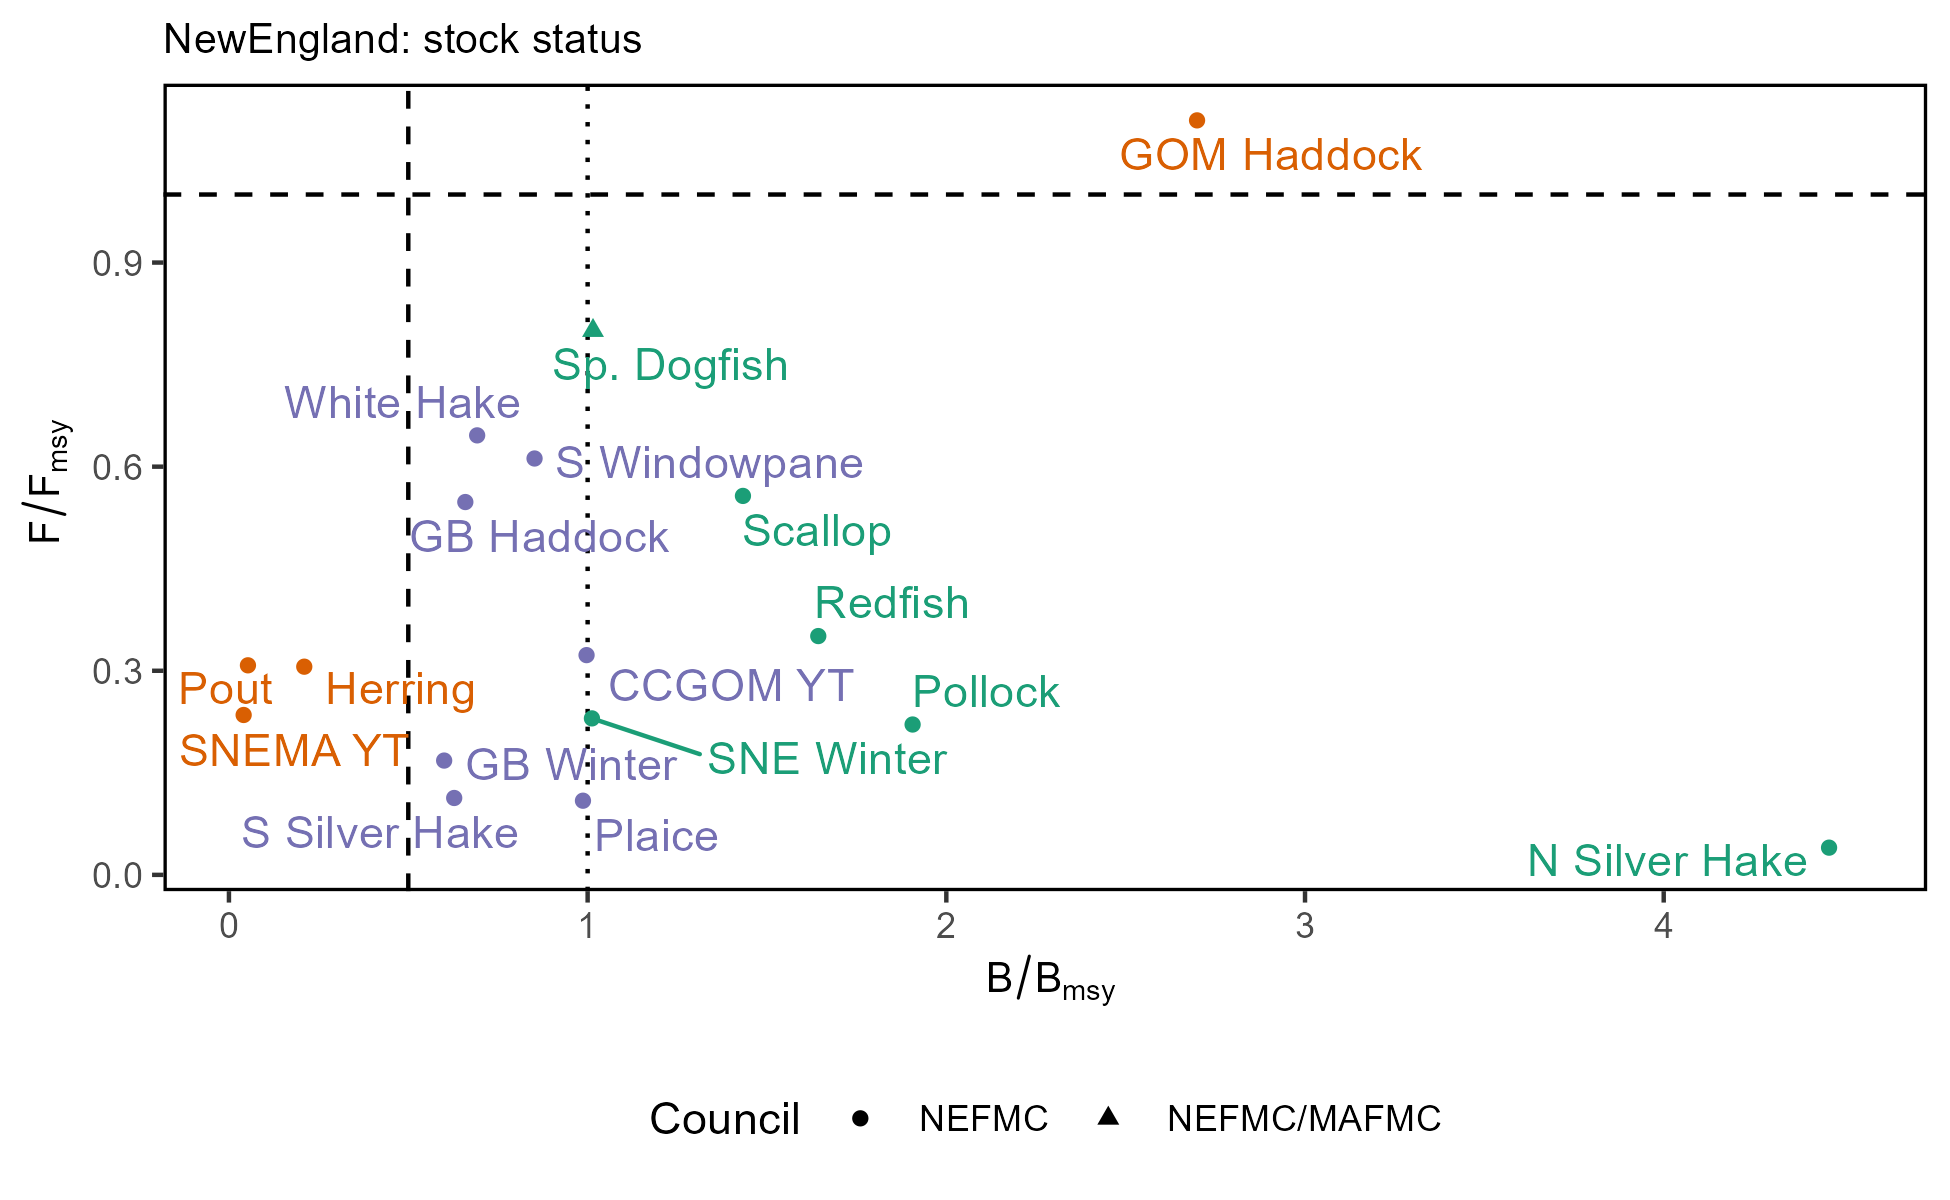
\includegraphics[width=6.5in]{images/NewEngland/stock_status_NewEngland_2025-09-09} 

}

\caption{Summary of single species status for NEFMC and jointly federally managed stocks (goosefish and spiny dogfish).  The dotted vertical line at one is the target biomass reference point of B.  The dashed lines are the management thresholds of B (vertical) or F (horizontal). Colors denote stocks with $B/B_{MSY}$ < 0.5 or $F/F_{MSY}$ (orange), stocks 0.5<$B/B_{MSY}$<1 (blue), and stocks $B/B_{MSY}$>1 (green).CCGOM = Cape Cod Gulf of Maine, GOM = Gulf of Maine, GB = Georges Bank, SNEMA = Southern New England Mid Atlantic}\label{fig:stock-status-51}
\end{figure}

\global\setlength{\Oldarrayrulewidth}{\arrayrulewidth}

\global\setlength{\Oldtabcolsep}{\tabcolsep}

\setlength{\tabcolsep}{2pt}

\renewcommand*{\arraystretch}{1}



\providecommand{\ascline}[3]{\noalign{\global\arrayrulewidth #1}\arrayrulecolor[HTML]{#2}\cline{#3}}

\begin{longtable}[c]{|p{3.43in}|p{0.75in}|p{0.75in}}

\caption{Unknown\ or\ partially\ known\ stock\ status\ for\ NEFMC\ and\ jointly\ managed\ species.}\label{tab:stock-status-table}\\

\ascline{1.5pt}{666666}{1-3}

\multicolumn{1}{>{\raggedright}m{\dimexpr 3.43in+0\tabcolsep}}{\textcolor[HTML]{000000}{\fontsize{9}{9}\selectfont{Stock}}} & \multicolumn{1}{>{\raggedleft}m{\dimexpr 0.75in+0\tabcolsep}}{\textcolor[HTML]{000000}{\fontsize{9}{9}\selectfont{F/Fmsy}}} & \multicolumn{1}{>{\raggedleft}m{\dimexpr 0.75in+0\tabcolsep}}{\textcolor[HTML]{000000}{\fontsize{9}{9}\selectfont{B/Bmsy}}} \\

\ascline{1.5pt}{666666}{1-3}\endfirsthead \caption[]{Unknown\ or\ partially\ known\ stock\ status\ for\ NEFMC\ and\ jointly\ managed\ species.}\label{tab:stock-status-table}\\

\ascline{1.5pt}{666666}{1-3}

\multicolumn{1}{>{\raggedright}m{\dimexpr 3.43in+0\tabcolsep}}{\textcolor[HTML]{000000}{\fontsize{9}{9}\selectfont{Stock}}} & \multicolumn{1}{>{\raggedleft}m{\dimexpr 0.75in+0\tabcolsep}}{\textcolor[HTML]{000000}{\fontsize{9}{9}\selectfont{F/Fmsy}}} & \multicolumn{1}{>{\raggedleft}m{\dimexpr 0.75in+0\tabcolsep}}{\textcolor[HTML]{000000}{\fontsize{9}{9}\selectfont{B/Bmsy}}} \\

\ascline{1.5pt}{666666}{1-3}\endhead



\multicolumn{3}{>{\raggedright}m{\dimexpr 4.93in+4\tabcolsep}}{\textcolor[HTML]{000000}{\fontsize{9}{9}\selectfont{\textsuperscript{1}}}\textcolor[HTML]{000000}{\fontsize{9}{9}\selectfont{The\ most\ recent\ cod\ assessment\ made\ stock\ status\ recommendations\ for\ the\ four\ new\ stocks\ (Eastern\ Gulf\ of\ Maine,\ Western\ Gulf\ of\ Maine,\ Georges\ Bank,\ and\ Southern\ New\ England)\ but\ were\ not\ available\ yet\ for\ this\ report.}}} \\

\endlastfoot



\multicolumn{1}{>{\raggedright}m{\dimexpr 3.43in+0\tabcolsep}}{\textcolor[HTML]{000000}{\fontsize{9}{9}\selectfont{Atlantic\ cod\ -\ Georges\ Bank}}\textcolor[HTML]{000000}{\fontsize{9}{9}\selectfont{\textsuperscript{1}}}} & \multicolumn{1}{>{\raggedleft}m{\dimexpr 0.75in+0\tabcolsep}}{\textcolor[HTML]{000000}{\fontsize{9}{9}\selectfont{-}}} & \multicolumn{1}{>{\raggedleft}m{\dimexpr 0.75in+0\tabcolsep}}{\textcolor[HTML]{000000}{\fontsize{9}{9}\selectfont{-}}} \\





\multicolumn{1}{>{\raggedright}m{\dimexpr 3.43in+0\tabcolsep}}{\textcolor[HTML]{000000}{\fontsize{9}{9}\selectfont{Atlantic\ cod\ -\ Gulf\ of\ Maine}}\textcolor[HTML]{000000}{\fontsize{9}{9}\selectfont{\textsuperscript{1}}}} & \multicolumn{1}{>{\raggedleft}m{\dimexpr 0.75in+0\tabcolsep}}{\textcolor[HTML]{000000}{\fontsize{9}{9}\selectfont{-}}} & \multicolumn{1}{>{\raggedleft}m{\dimexpr 0.75in+0\tabcolsep}}{\textcolor[HTML]{000000}{\fontsize{9}{9}\selectfont{-}}} \\





\multicolumn{1}{>{\raggedright}m{\dimexpr 3.43in+0\tabcolsep}}{\textcolor[HTML]{000000}{\fontsize{9}{9}\selectfont{Atlantic\ halibut\ -\ Northwestern\ Atlantic\ Coast}}} & \multicolumn{1}{>{\raggedleft}m{\dimexpr 0.75in+0\tabcolsep}}{\textcolor[HTML]{000000}{\fontsize{9}{9}\selectfont{-}}} & \multicolumn{1}{>{\raggedleft}m{\dimexpr 0.75in+0\tabcolsep}}{\textcolor[HTML]{000000}{\fontsize{9}{9}\selectfont{-}}} \\





\multicolumn{1}{>{\raggedright}m{\dimexpr 3.43in+0\tabcolsep}}{\textcolor[HTML]{000000}{\fontsize{9}{9}\selectfont{Barndoor\ skate\ -\ Georges\ Bank\ /\ Southern\ New\ England}}} & \multicolumn{1}{>{\raggedleft}m{\dimexpr 0.75in+0\tabcolsep}}{\textcolor[HTML]{000000}{\fontsize{9}{9}\selectfont{-}}} & \multicolumn{1}{>{\raggedleft}m{\dimexpr 0.75in+0\tabcolsep}}{\textcolor[HTML]{000000}{\fontsize{9}{9}\selectfont{1.070}}} \\





\multicolumn{1}{>{\raggedright}m{\dimexpr 3.43in+0\tabcolsep}}{\textcolor[HTML]{000000}{\fontsize{9}{9}\selectfont{Clearnose\ skate\ -\ Southern\ New\ England\ /\ Mid-Atlantic}}} & \multicolumn{1}{>{\raggedleft}m{\dimexpr 0.75in+0\tabcolsep}}{\textcolor[HTML]{000000}{\fontsize{9}{9}\selectfont{-}}} & \multicolumn{1}{>{\raggedleft}m{\dimexpr 0.75in+0\tabcolsep}}{\textcolor[HTML]{000000}{\fontsize{9}{9}\selectfont{0.802}}} \\





\multicolumn{1}{>{\raggedright}m{\dimexpr 3.43in+0\tabcolsep}}{\textcolor[HTML]{000000}{\fontsize{9}{9}\selectfont{Little\ skate\ -\ Georges\ Bank\ /\ Southern\ New\ England}}} & \multicolumn{1}{>{\raggedleft}m{\dimexpr 0.75in+0\tabcolsep}}{\textcolor[HTML]{000000}{\fontsize{9}{9}\selectfont{-}}} & \multicolumn{1}{>{\raggedleft}m{\dimexpr 0.75in+0\tabcolsep}}{\textcolor[HTML]{000000}{\fontsize{9}{9}\selectfont{0.580}}} \\





\multicolumn{1}{>{\raggedright}m{\dimexpr 3.43in+0\tabcolsep}}{\textcolor[HTML]{000000}{\fontsize{9}{9}\selectfont{Offshore\ hake\ -\ Northwestern\ Atlantic\ Coast}}} & \multicolumn{1}{>{\raggedleft}m{\dimexpr 0.75in+0\tabcolsep}}{\textcolor[HTML]{000000}{\fontsize{9}{9}\selectfont{-}}} & \multicolumn{1}{>{\raggedleft}m{\dimexpr 0.75in+0\tabcolsep}}{\textcolor[HTML]{000000}{\fontsize{9}{9}\selectfont{-}}} \\





\multicolumn{1}{>{\raggedright}m{\dimexpr 3.43in+0\tabcolsep}}{\textcolor[HTML]{000000}{\fontsize{9}{9}\selectfont{Red\ deepsea\ crab\ -\ Northwestern\ Atlantic}}} & \multicolumn{1}{>{\raggedleft}m{\dimexpr 0.75in+0\tabcolsep}}{\textcolor[HTML]{000000}{\fontsize{9}{9}\selectfont{-}}} & \multicolumn{1}{>{\raggedleft}m{\dimexpr 0.75in+0\tabcolsep}}{\textcolor[HTML]{000000}{\fontsize{9}{9}\selectfont{-}}} \\





\multicolumn{1}{>{\raggedright}m{\dimexpr 3.43in+0\tabcolsep}}{\textcolor[HTML]{000000}{\fontsize{9}{9}\selectfont{Red\ hake\ -\ Gulf\ of\ Maine\ /\ Northern\ Georges\ Bank}}} & \multicolumn{1}{>{\raggedleft}m{\dimexpr 0.75in+0\tabcolsep}}{\textcolor[HTML]{000000}{\fontsize{9}{9}\selectfont{-}}} & \multicolumn{1}{>{\raggedleft}m{\dimexpr 0.75in+0\tabcolsep}}{\textcolor[HTML]{000000}{\fontsize{9}{9}\selectfont{-}}} \\





\multicolumn{1}{>{\raggedright}m{\dimexpr 3.43in+0\tabcolsep}}{\textcolor[HTML]{000000}{\fontsize{9}{9}\selectfont{Red\ hake\ -\ Southern\ Georges\ Bank\ /\ Mid-Atlantic}}} & \multicolumn{1}{>{\raggedleft}m{\dimexpr 0.75in+0\tabcolsep}}{\textcolor[HTML]{000000}{\fontsize{9}{9}\selectfont{-}}} & \multicolumn{1}{>{\raggedleft}m{\dimexpr 0.75in+0\tabcolsep}}{\textcolor[HTML]{000000}{\fontsize{9}{9}\selectfont{-}}} \\





\multicolumn{1}{>{\raggedright}m{\dimexpr 3.43in+0\tabcolsep}}{\textcolor[HTML]{000000}{\fontsize{9}{9}\selectfont{Rosette\ skate\ -\ Southern\ New\ England\ /\ Mid-Atlantic}}} & \multicolumn{1}{>{\raggedleft}m{\dimexpr 0.75in+0\tabcolsep}}{\textcolor[HTML]{000000}{\fontsize{9}{9}\selectfont{-}}} & \multicolumn{1}{>{\raggedleft}m{\dimexpr 0.75in+0\tabcolsep}}{\textcolor[HTML]{000000}{\fontsize{9}{9}\selectfont{1.075}}} \\





\multicolumn{1}{>{\raggedright}m{\dimexpr 3.43in+0\tabcolsep}}{\textcolor[HTML]{000000}{\fontsize{9}{9}\selectfont{Smooth\ skate\ -\ Gulf\ of\ Maine}}} & \multicolumn{1}{>{\raggedleft}m{\dimexpr 0.75in+0\tabcolsep}}{\textcolor[HTML]{000000}{\fontsize{9}{9}\selectfont{-}}} & \multicolumn{1}{>{\raggedleft}m{\dimexpr 0.75in+0\tabcolsep}}{\textcolor[HTML]{000000}{\fontsize{9}{9}\selectfont{0.696}}} \\





\multicolumn{1}{>{\raggedright}m{\dimexpr 3.43in+0\tabcolsep}}{\textcolor[HTML]{000000}{\fontsize{9}{9}\selectfont{Thorny\ skate\ -\ Gulf\ of\ Maine}}} & \multicolumn{1}{>{\raggedleft}m{\dimexpr 0.75in+0\tabcolsep}}{\textcolor[HTML]{000000}{\fontsize{9}{9}\selectfont{-}}} & \multicolumn{1}{>{\raggedleft}m{\dimexpr 0.75in+0\tabcolsep}}{\textcolor[HTML]{000000}{\fontsize{9}{9}\selectfont{0.035}}} \\





\multicolumn{1}{>{\raggedright}m{\dimexpr 3.43in+0\tabcolsep}}{\textcolor[HTML]{000000}{\fontsize{9}{9}\selectfont{Windowpane\ -\ Gulf\ of\ Maine\ /\ Georges\ Bank}}} & \multicolumn{1}{>{\raggedleft}m{\dimexpr 0.75in+0\tabcolsep}}{\textcolor[HTML]{000000}{\fontsize{9}{9}\selectfont{-}}} & \multicolumn{1}{>{\raggedleft}m{\dimexpr 0.75in+0\tabcolsep}}{\textcolor[HTML]{000000}{\fontsize{9}{9}\selectfont{-}}} \\





\multicolumn{1}{>{\raggedright}m{\dimexpr 3.43in+0\tabcolsep}}{\textcolor[HTML]{000000}{\fontsize{9}{9}\selectfont{Winter\ flounder\ -\ Gulf\ of\ Maine}}} & \multicolumn{1}{>{\raggedleft}m{\dimexpr 0.75in+0\tabcolsep}}{\textcolor[HTML]{000000}{\fontsize{9}{9}\selectfont{-}}} & \multicolumn{1}{>{\raggedleft}m{\dimexpr 0.75in+0\tabcolsep}}{\textcolor[HTML]{000000}{\fontsize{9}{9}\selectfont{-}}} \\





\multicolumn{1}{>{\raggedright}m{\dimexpr 3.43in+0\tabcolsep}}{\textcolor[HTML]{000000}{\fontsize{9}{9}\selectfont{Winter\ skate\ -\ Georges\ Bank\ /\ Southern\ New\ England}}} & \multicolumn{1}{>{\raggedleft}m{\dimexpr 0.75in+0\tabcolsep}}{\textcolor[HTML]{000000}{\fontsize{9}{9}\selectfont{-}}} & \multicolumn{1}{>{\raggedleft}m{\dimexpr 0.75in+0\tabcolsep}}{\textcolor[HTML]{000000}{\fontsize{9}{9}\selectfont{1.120}}} \\





\multicolumn{1}{>{\raggedright}m{\dimexpr 3.43in+0\tabcolsep}}{\textcolor[HTML]{000000}{\fontsize{9}{9}\selectfont{Witch\ flounder\ -\ Northwestern\ Atlantic\ Coast}}} & \multicolumn{1}{>{\raggedleft}m{\dimexpr 0.75in+0\tabcolsep}}{\textcolor[HTML]{000000}{\fontsize{9}{9}\selectfont{-}}} & \multicolumn{1}{>{\raggedleft}m{\dimexpr 0.75in+0\tabcolsep}}{\textcolor[HTML]{000000}{\fontsize{9}{9}\selectfont{-}}} \\





\multicolumn{1}{>{\raggedright}m{\dimexpr 3.43in+0\tabcolsep}}{\textcolor[HTML]{000000}{\fontsize{9}{9}\selectfont{Yellowtail\ flounder\ -\ Georges\ Bank}}} & \multicolumn{1}{>{\raggedleft}m{\dimexpr 0.75in+0\tabcolsep}}{\textcolor[HTML]{000000}{\fontsize{9}{9}\selectfont{0.09}}} & \multicolumn{1}{>{\raggedleft}m{\dimexpr 0.75in+0\tabcolsep}}{\textcolor[HTML]{000000}{\fontsize{9}{9}\selectfont{-}}} \\





\multicolumn{1}{>{\raggedright}m{\dimexpr 3.43in+0\tabcolsep}}{\textcolor[HTML]{000000}{\fontsize{9}{9}\selectfont{Goosefish\ -\ Gulf\ of\ Maine\ /\ Northern\ Georges\ Bank}}} & \multicolumn{1}{>{\raggedleft}m{\dimexpr 0.75in+0\tabcolsep}}{\textcolor[HTML]{000000}{\fontsize{9}{9}\selectfont{-}}} & \multicolumn{1}{>{\raggedleft}m{\dimexpr 0.75in+0\tabcolsep}}{\textcolor[HTML]{000000}{\fontsize{9}{9}\selectfont{-}}} \\





\multicolumn{1}{>{\raggedright}m{\dimexpr 3.43in+0\tabcolsep}}{\textcolor[HTML]{000000}{\fontsize{9}{9}\selectfont{Goosefish\ -\ Southern\ Georges\ Bank\ /\ Mid-Atlantic}}} & \multicolumn{1}{>{\raggedleft}m{\dimexpr 0.75in+0\tabcolsep}}{\textcolor[HTML]{000000}{\fontsize{9}{9}\selectfont{-}}} & \multicolumn{1}{>{\raggedleft}m{\dimexpr 0.75in+0\tabcolsep}}{\textcolor[HTML]{000000}{\fontsize{9}{9}\selectfont{-}}} \\

\ascline{1.5pt}{666666}{1-3}



\end{longtable}



\arrayrulecolor[HTML]{000000}

\global\setlength{\arrayrulewidth}{\Oldarrayrulewidth}

\global\setlength{\tabcolsep}{\Oldtabcolsep}

\renewcommand*{\arraystretch}{1}

\paragraph{System Biomass}\label{system-biomass-1}

\href{https://noaa-edab.github.io/catalog/aggregate_biomass.html}{Aggregate biomass} trends derived from scientific resource surveys have been stable to increasing in both regions (Fig. \ref{fig:nefsc-biomass-gb} \& Fig. \ref{fig:nefsc-biomass-gom}).The benthivores group spiked during the last decade, due to a large haddock recruitment, but appears to be returning to average levels. Planktivore biomass on GB continues to rise with the highest fall biomass observed since 1968. There are mixed trends in piscivores on GB, and increasing trends for planktivores across both regions and seasons and benthos on GB in both seasons. The New Hampshire/Maine state survey time series is too short to estimate trends, while the Massachusetts state survey shows the increasing trend in planktivores in the fall but a decrease in piscivores in the spring and benthos in both seasons (Fig. \ref{fig:mass-biomass}). While managed species comprise varying proportions of aggregate biomass, trends in landings are not mirroring shifts in the overall trophic structure of survey-sampled fish and invertebrates. Therefore, major shifts in feeding guilds or ecosystem trophic structure are unlikely to be driving the decline in landings.

\paragraph{Effect on Seafood Production}\label{effect-on-seafood-production-1}

With the poor or unknown stock status of many managed species, the decline in commercial seafood landings in the Gulf of Maine most likely reflects lower catch quotas implemented to rebuild overfished stocks, as well as market dynamics.

The decline in recreational seafood harvest stems from multiple drivers. Some of the decline, such as for recreational shark landings, continues to be driven by tightening regulations. However, changes in demographics and preferences for recreational activities likely play a role in non-HMS (Highly Migratory Species) declines in recreational harvest, with current harvests well below the time series average.

Other environmental changes require monitoring as they may become important drivers of future landings:

\begin{itemize}
\tightlist
\item
  Climate is trending into uncharted territory. Globally, 2024 was the warmest year on record\footnote{\url{https://noaa-edab.github.io/catalog/observation_synthesis.html}} (see \hyperref[highlights]{2024 Highlights section}).
\item
  Stocks are shifting their distribution, moving towards the northeast and into deeper waters throughout the Northeast US Large Marine Ecosystem (Fig. \ref{fig:species-dist}, \hyperref[climate-risks]{Climate Risks section}).
\item
  Ecosystem composition and production changes have been observed (see \hyperref[stability]{Stability section}).
\item
  Some fishing communities are affected by social vulnerabilities (see \hyperref[social-vulnerability]{Social Vulnerability section}).
\end{itemize}

\newpage

\section{parent\_report.Rmd}\label{parent_report.rmd-2}

\subsection{Commercial Profits}\label{commercial-profits}

\section{02\_commercial\_profits\_midatlantic.Rmd}\label{commercial_profits_midatlantic.rmd}

\subsubsection{Indicators: revenue (a proxy for profits)}\label{indicators-revenue-a-proxy-for-profits}

Total \href{https://noaa-edab.github.io/catalog/comdat.html}{commercial revenue} and MAFMC managed species revenue within the Mid-Atlantic Bight have declined over the past 20-30 years. In 2023, total revenue was at an all-time low, and revenue from MAFMC managed species was near an all-time low (Fig. \ref{fig:comm-revenue}).

\begin{figure}

{\centering 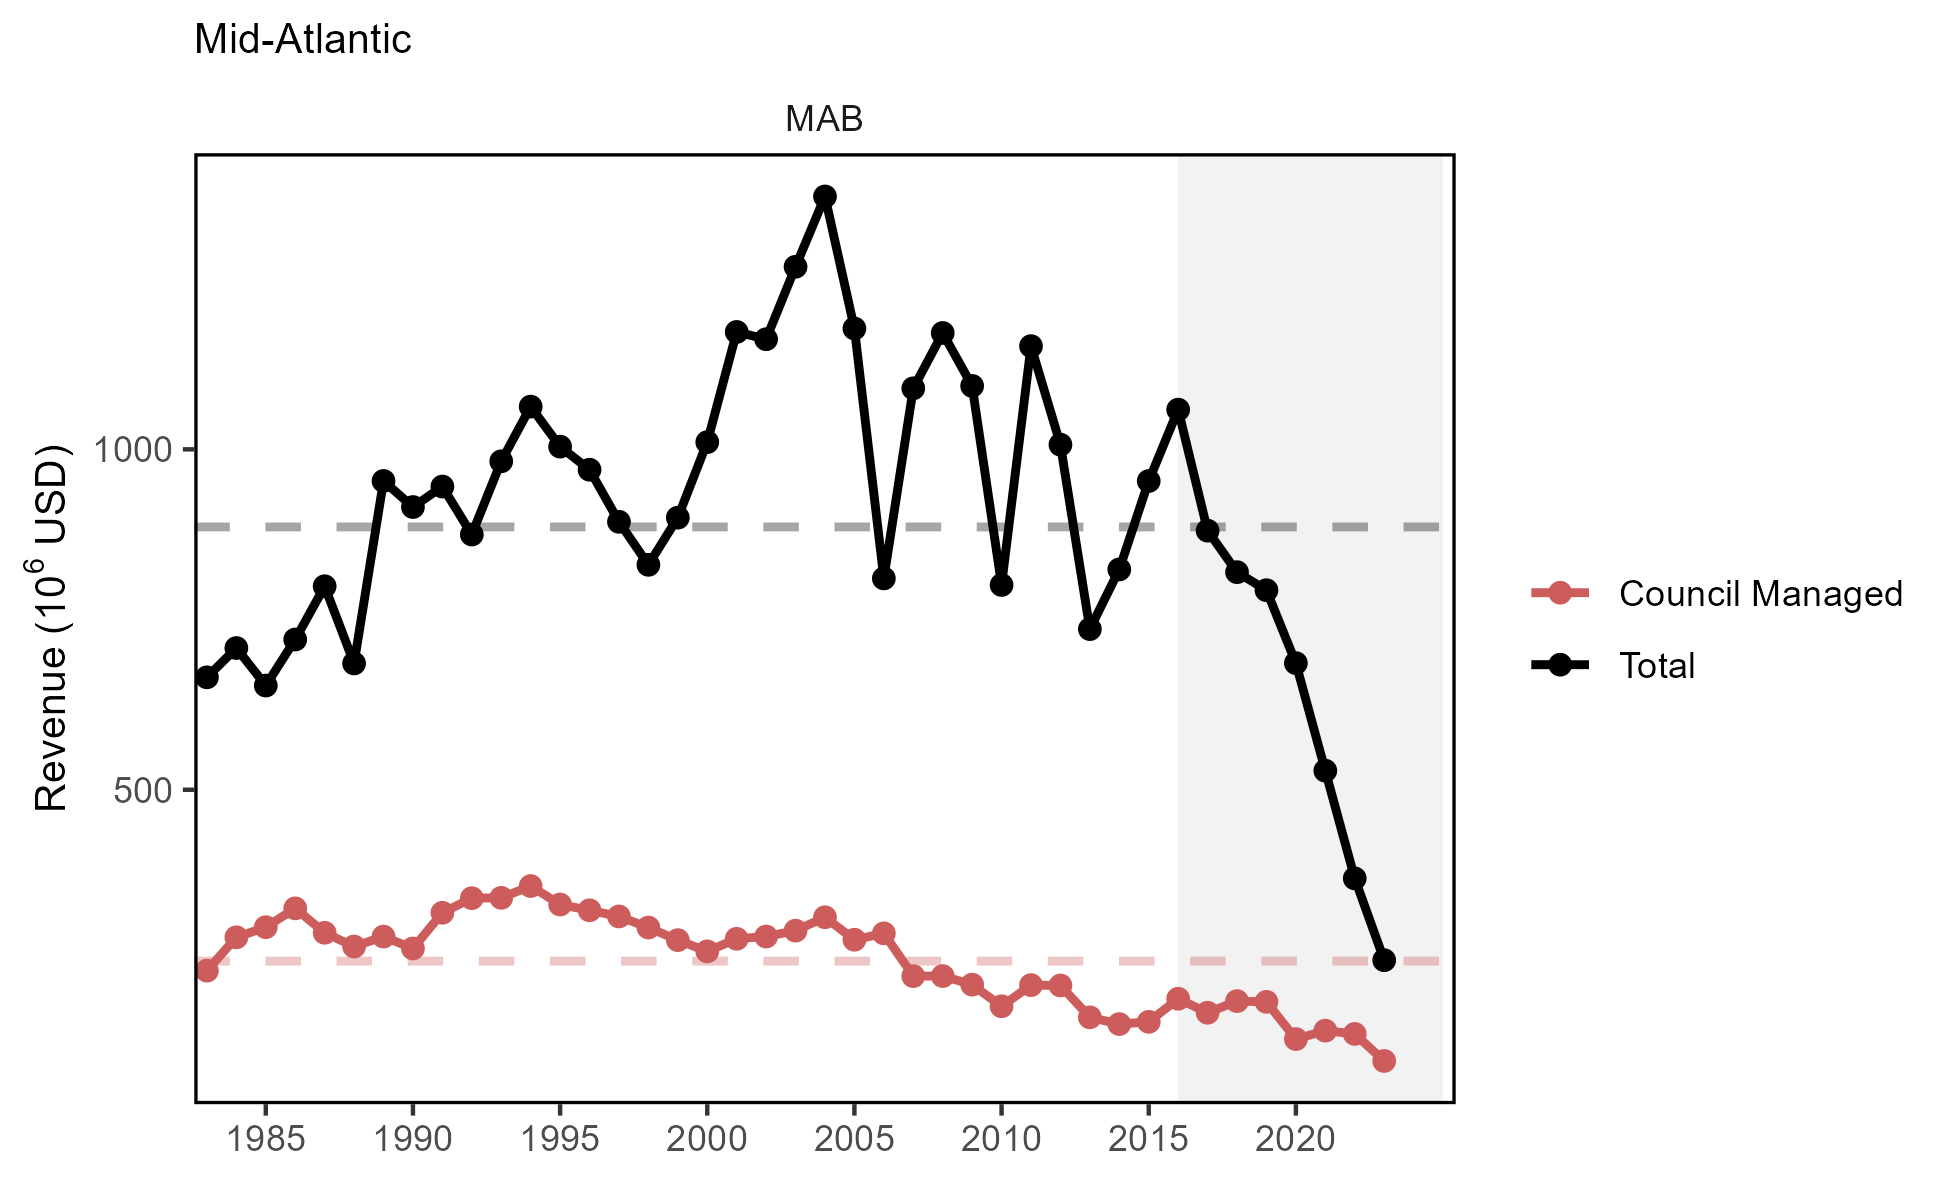
\includegraphics[width=6.5in]{images/MidAtlantic/comm_revenue_MidAtlantic_2025-09-05} 

}

\caption{Revenue for the for the Mid-Atlantic region: total (black) and from MAFMC managed species (red).}\label{fig:comm-revenue}
\end{figure}

Revenue earned by harvesting resources is a function of both the quantity landed of each species and the prices paid for landings. Beyond monitoring yearly changes in revenue, it is even more valuable to determine what drives these changes: harvest levels, the mix of species landed, price changes, or a combination of these. The \href{https://noaa-edab.github.io/catalog/bennet.html}{Bennet Indicator} decomposes revenue change into two parts, one driven by changing quantities (volumes), and a second driven by changing prices. All changes are in relation to a base year (1982). The 1982 base year was selected because that is the first year the relevant data is available and it also allows for an extended period of time in which to evaluate market trends and dynamics.

In the Mid-Atlantic region revenues were above the 1982 baseline for all years in the series until 2022 and 2023 (Fig. \ref{fig:bennet}). In 2023, lower revenue was driven primarily by both lower quantities of benthos landed, and lower prices of benthos, benthivores, and planktivores. The lower benthos prices are a departure from past years, which saw benthos prices contributing positively to revenue changes since the early 2000's. (Fig. \ref{fig:bennet-all}).

\begin{figure}

{\centering 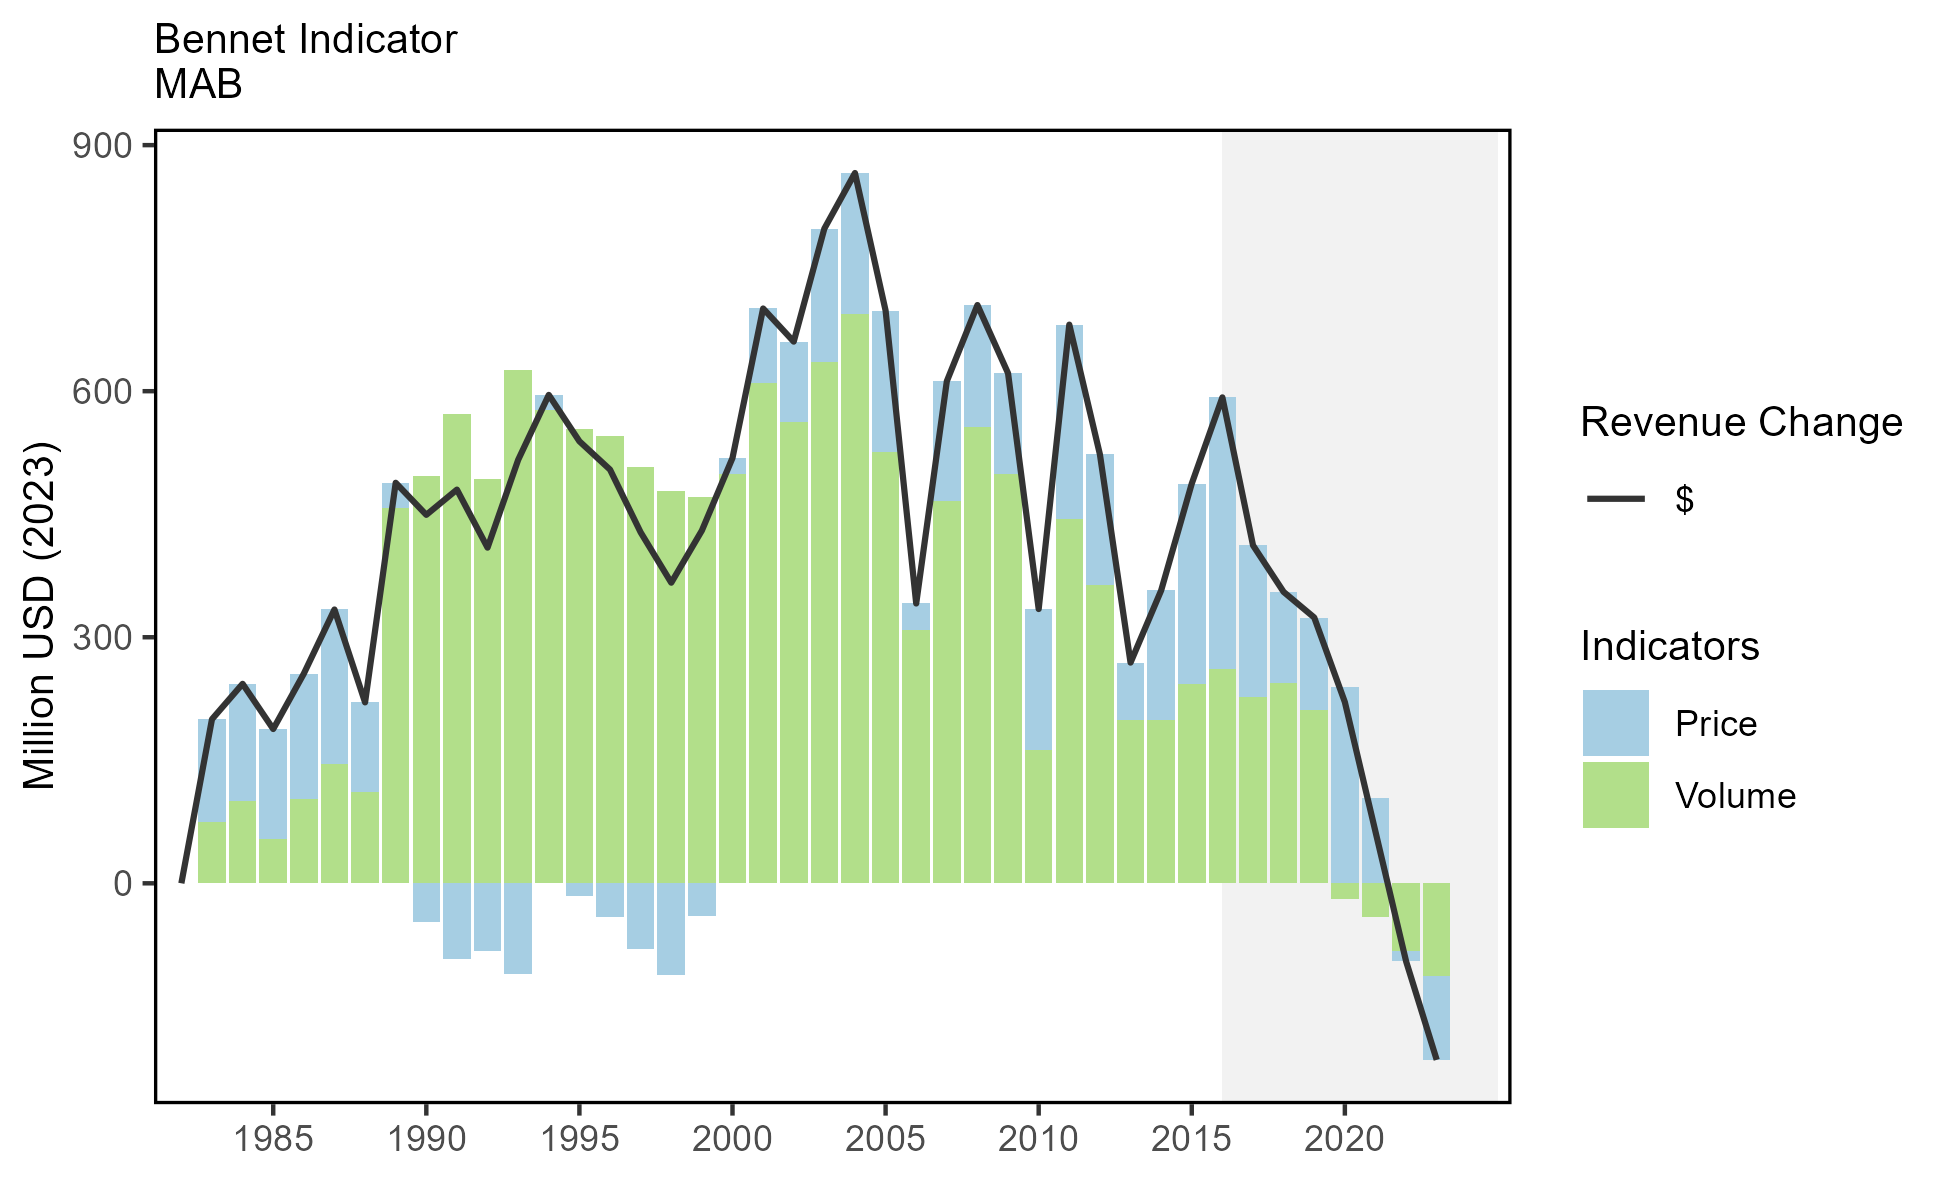
\includegraphics[width=6.5in]{images/MidAtlantic/bennet_MidAtlantic_2025-09-05} 

}

\caption{Revenue change from 1982 values in 2023 dollars (black); Price (PI), and Volume Indicators (VI) for total commercial landings in the Mid-Atlantic Bight.}\label{fig:bennet}
\end{figure}

\begin{figure}

{\centering 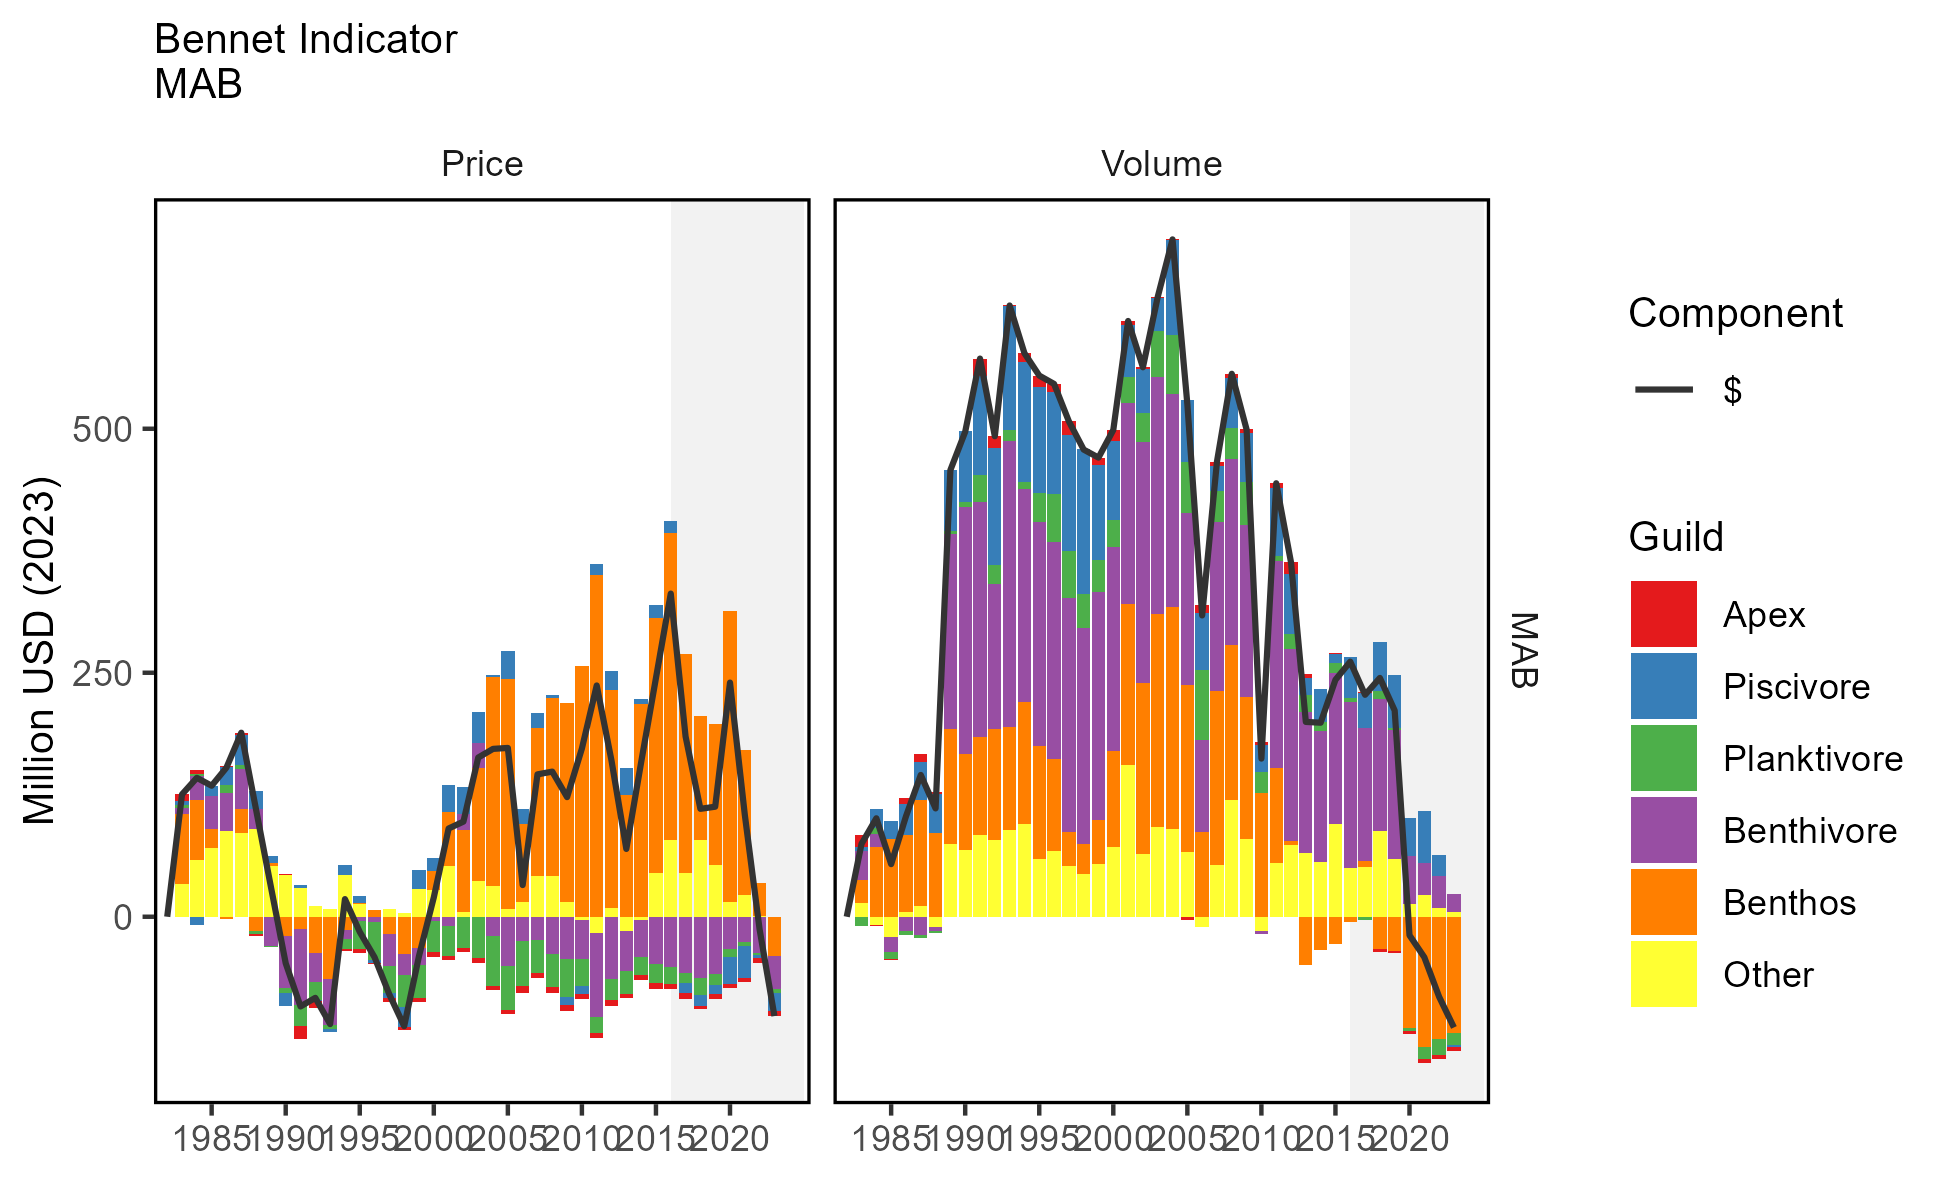
\includegraphics[width=6.5in]{images/MidAtlantic/bennet_all_MidAtlantic_2025-09-05} 

}

\caption{Total price and volume indicators in 2023 dollars (black) for commercial landings, and individual guild contributions to each indicator, in the Mid-Atlantic Bight.}\label{fig:bennet-all}
\end{figure}

For ports combined across Mid-Atlantic states, \href{https://noaa-edab.github.io/catalog/community_climate_vulnerability.html}{total climate vulnerability} of revenue ranged from high to very high from 2000-2021, with no long-term trend. This suggests that Mid-Atlantic port commercial fishing revenue has been highly reliant on climate-sensitive species for most of the period since 2000 (Fig. \ref{fig:climatevul-rev}).

\begin{figure}

{\centering 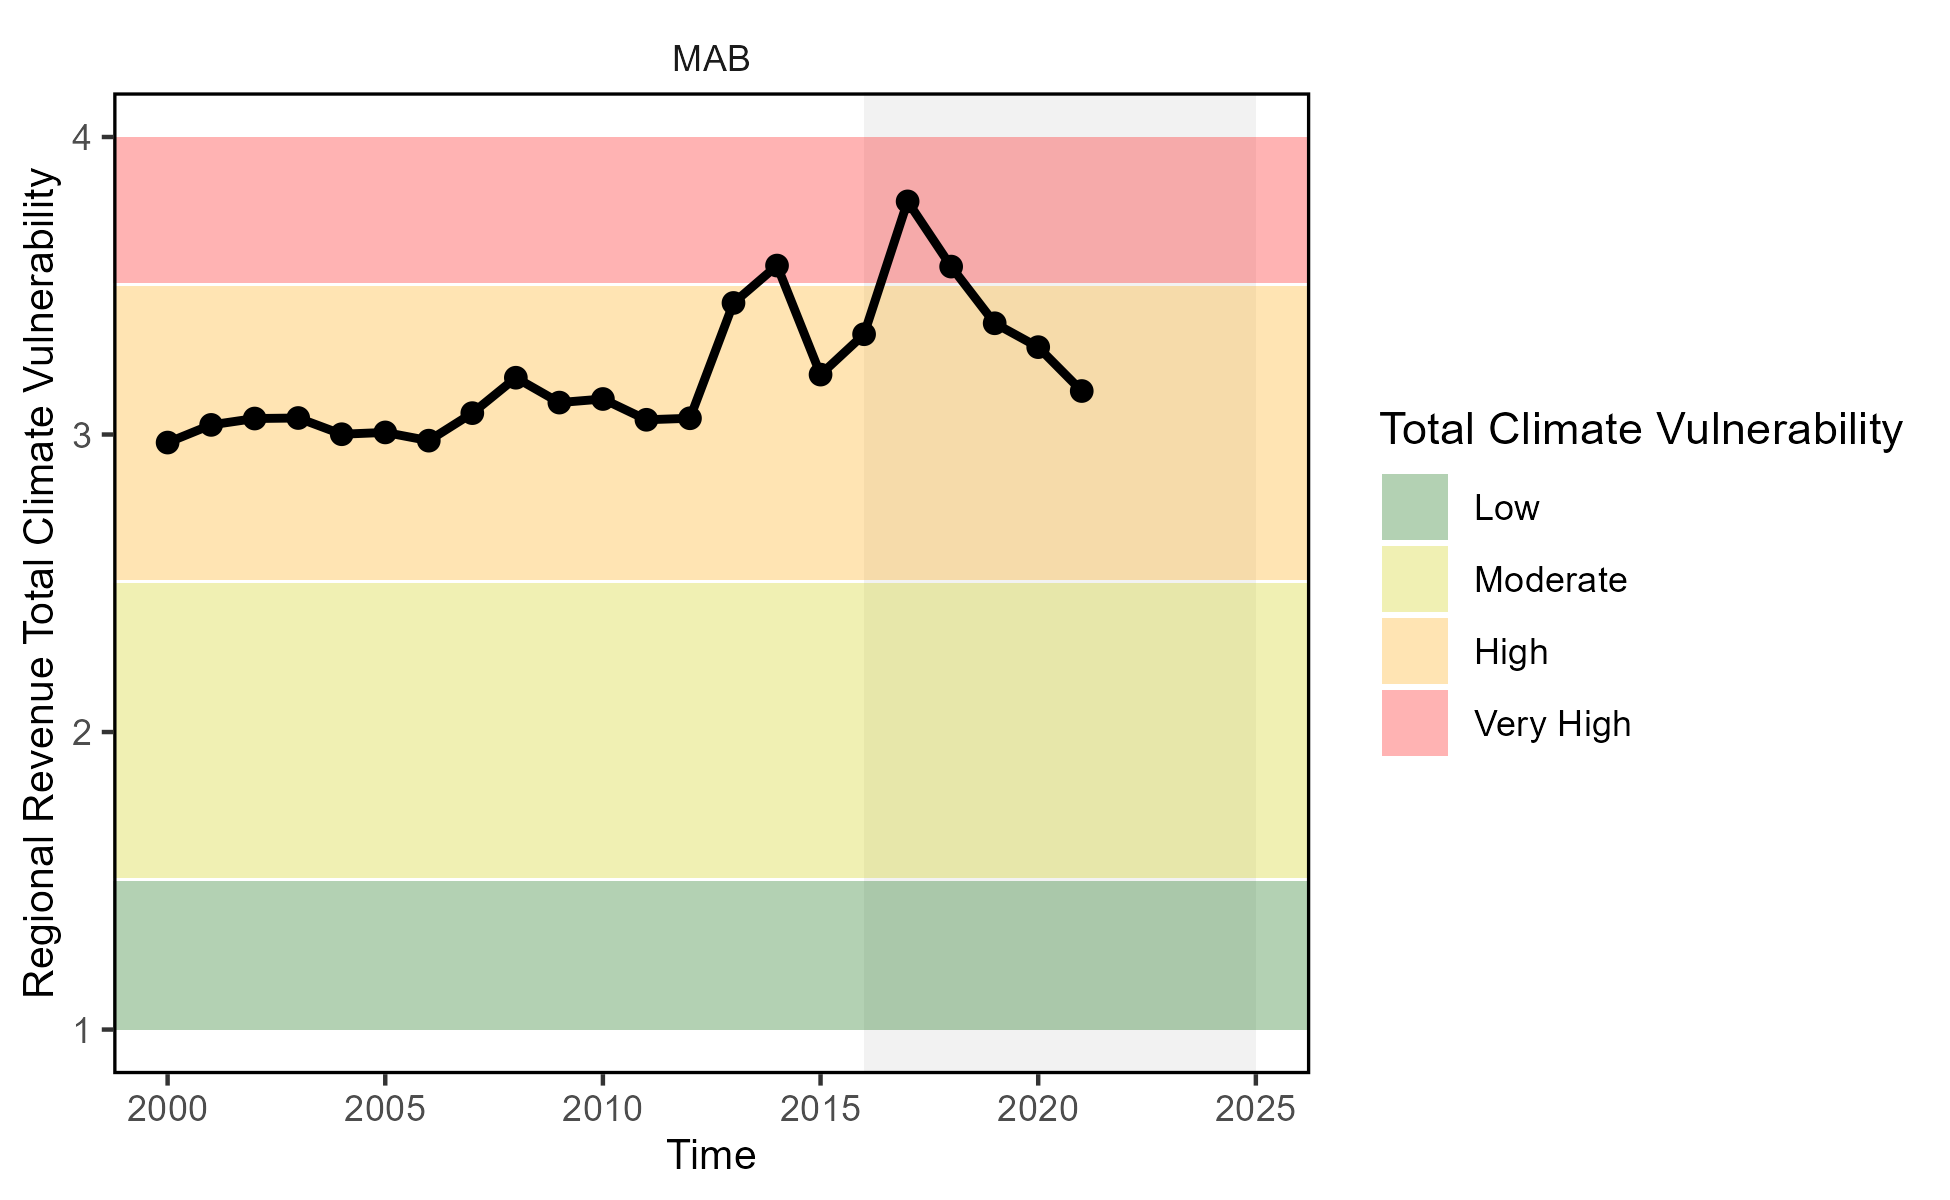
\includegraphics[width=6.5in]{images/MidAtlantic/climatevul_rev_MidAtlantic_2025-09-05} 

}

\caption{Mid-Atlantic region total climate vulnerability of commercial revenue (sum of Mid-Atlantic port revenue weighted by species climate vulnerability from Hare et al. 2016).}\label{fig:climatevul-rev}
\end{figure}

\subsubsection{Implications}\label{implications-2}

Although the Mid-Atlantic region shows declining revenue since 2016, inflation-adjusted revenue from harvested species was still greater than 1982 levels until the past two years. In a similar manner to seafood landings, the results here are driven in large part by market dynamics affecting the landings of surfclams and ocean quahogs, as landings have been below quotas for these species, as well as lower quotas and prices for Atlantic scallops. The declining benthos category since 2012 may be partially caused by decreases in surfclam and ocean quahogs in the southern part of their range as harvest have shifted northward. Changes in other indicators, particularly those driving landings and those related to climate change, require monitoring as they may become important drivers of revenue in the future; for example:

\begin{itemize}
\tightlist
\item
  Surfclams, ocean quahogs, and scallops are sensitive to warming ocean temperatures and ocean acidification, as reflected in the high climate vulnerability of total landings from from Mid-Atlantic ports.
\item
  Multiple stressors including \href{https://noaa-edab.github.io/catalog/bottom_temp_insitu.html}{warming} and \href{https://noaa-edab.github.io/catalog/ocean_acidification}{ocean acidification} are interacting in Mid-Atlantic shellfish habitats.
\end{itemize}

\section{parent\_report.Rmd}\label{parent_report.rmd-3}

\section{02\_commercial\_profits\_newengland.Rmd}\label{commercial_profits_newengland.rmd}

\subsubsection{Indicators: revenue (a proxy for profits)}\label{indicators-revenue-a-proxy-for-profits-1}

Total \href{https://noaa-edab.github.io/catalog/comdat.html}{commercial revenues} from all species is below the long-term mean for both the GB and GOM regions in 2023 (Fig. \ref{fig:comm-revenue}). In addition, revenue from NEFMC managed species shows a long-term decline in the GOM. GB continues to exhibit a cyclical nature with regards to revenue, largely driven by rotational management of Atlantic sea

\begin{figure}

{\centering 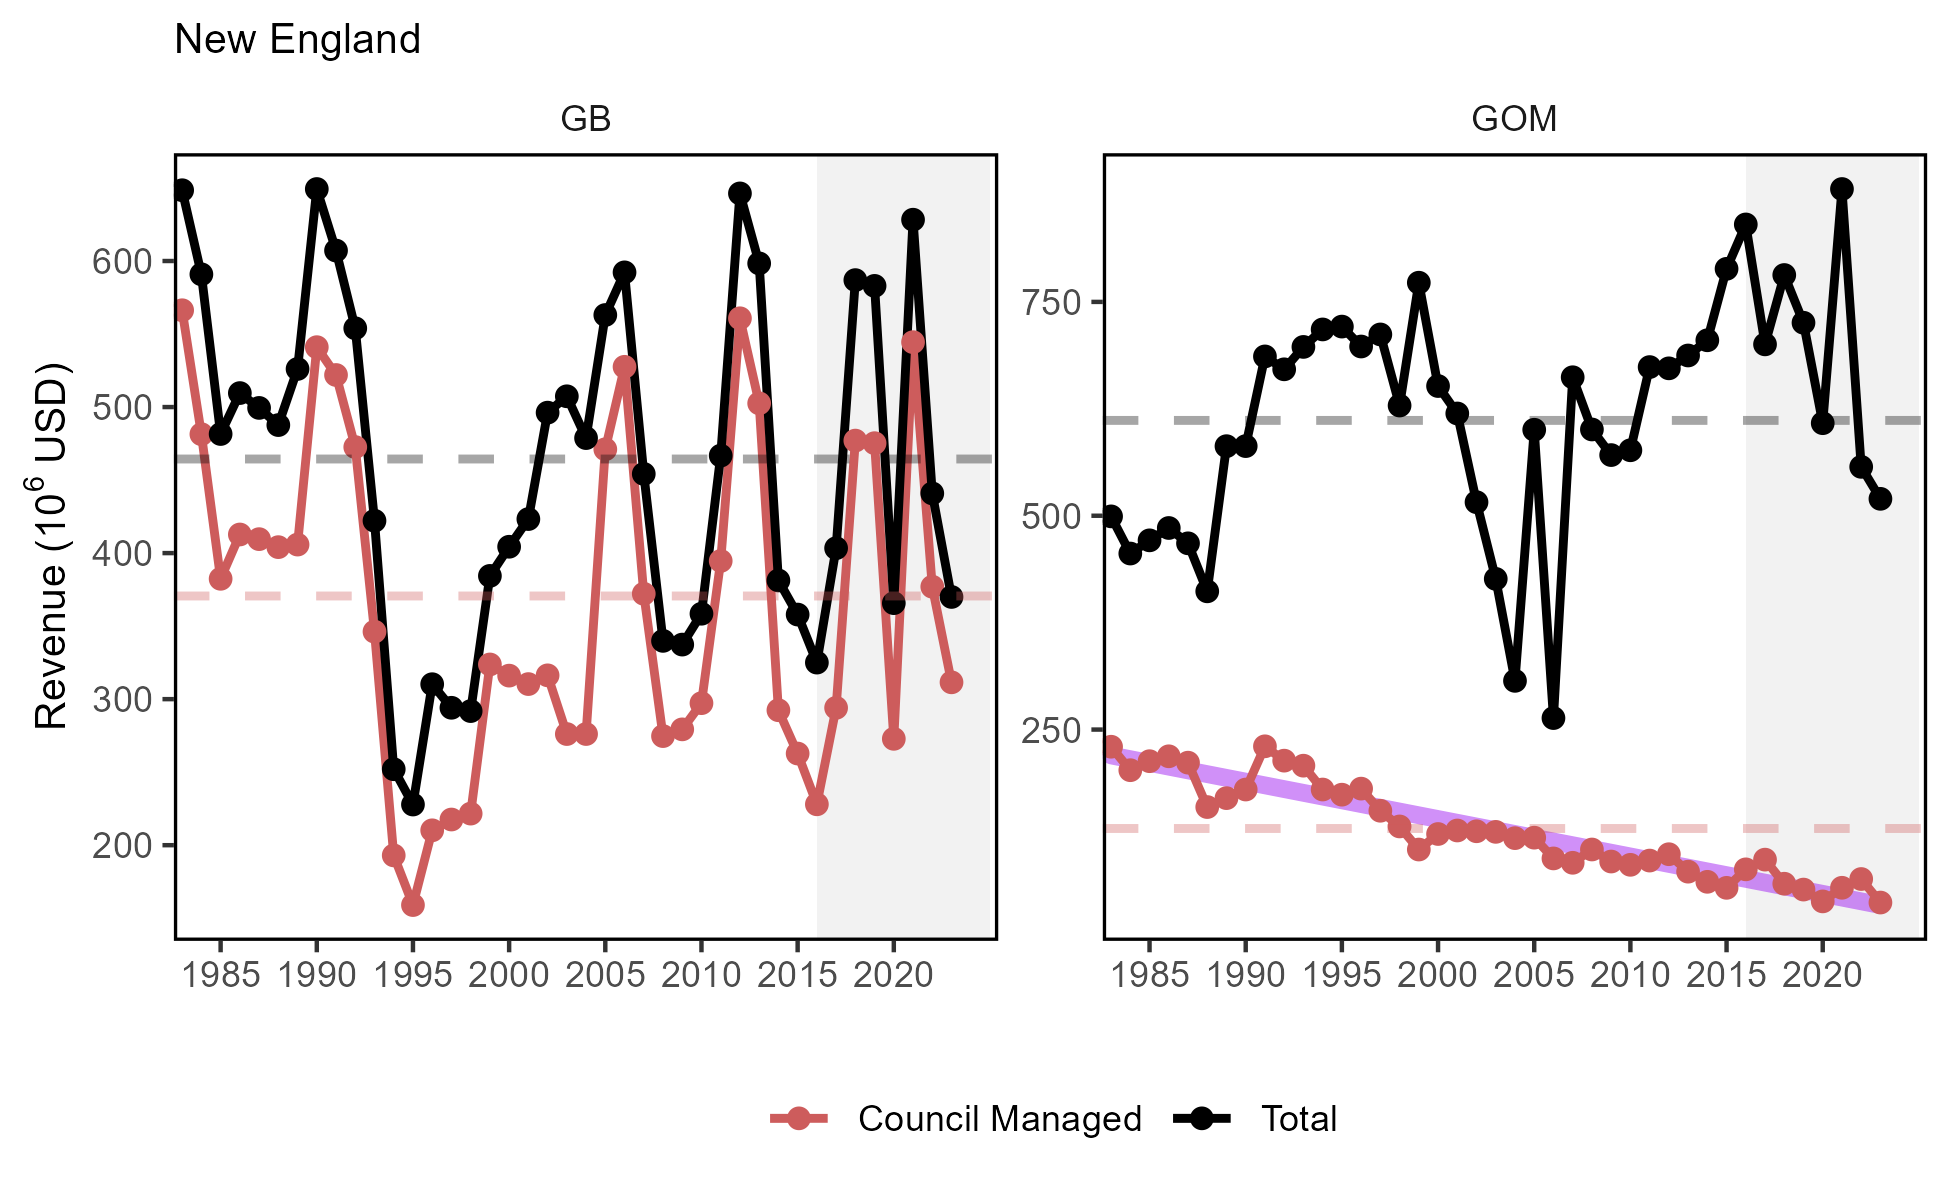
\includegraphics[width=6.5in]{images/NewEngland/comm_revenue_NewEngland_2025-09-09} 

}

\caption{Revenue through 2023 for the New England region: total (black) and from NEFMC managed species (red).}\label{fig:comm-revenue-81}
\end{figure}

Revenue earned by harvesting resources is a function of both the quantity landed of each species and the prices paid for landings. Beyond monitoring yearly changes in revenue, it is even more valuable to determine what drives these changes: harvest levels, the mix of species landed, price changes, or a combination of these. The \href{https://noaa-edab.github.io/catalog/bennet.html}{Bennet Indicator} decomposes revenue change into two parts, one driven by changing quantities (volumes), and a second driven by changing prices. All changes are in relation to a base year (1982).

In the GB region, revenues have been consistently lower than the 1982 baseline throughout the time series. The changes in total revenue in GB was primarily driven by volumes prior to 2010, and then by prices (Fig.\ref{fig:bennet}). In the GOM, revenues have been above the 1982 baseline in all but four years, largely due to changing prices in most years. Breaking down the revenue by guild (Fig. \ref{fig:bennet-all}), or GB, both the volume and price trend have been largely driven by benthos (scallops, quahogs and surfclams). In the GOM region, increased prices for benthivores (lobster) drove the year-over-year increases in overall prices. Benthivores also had a large influence on the overall volume indicator in the GOM.

\begin{figure}

{\centering 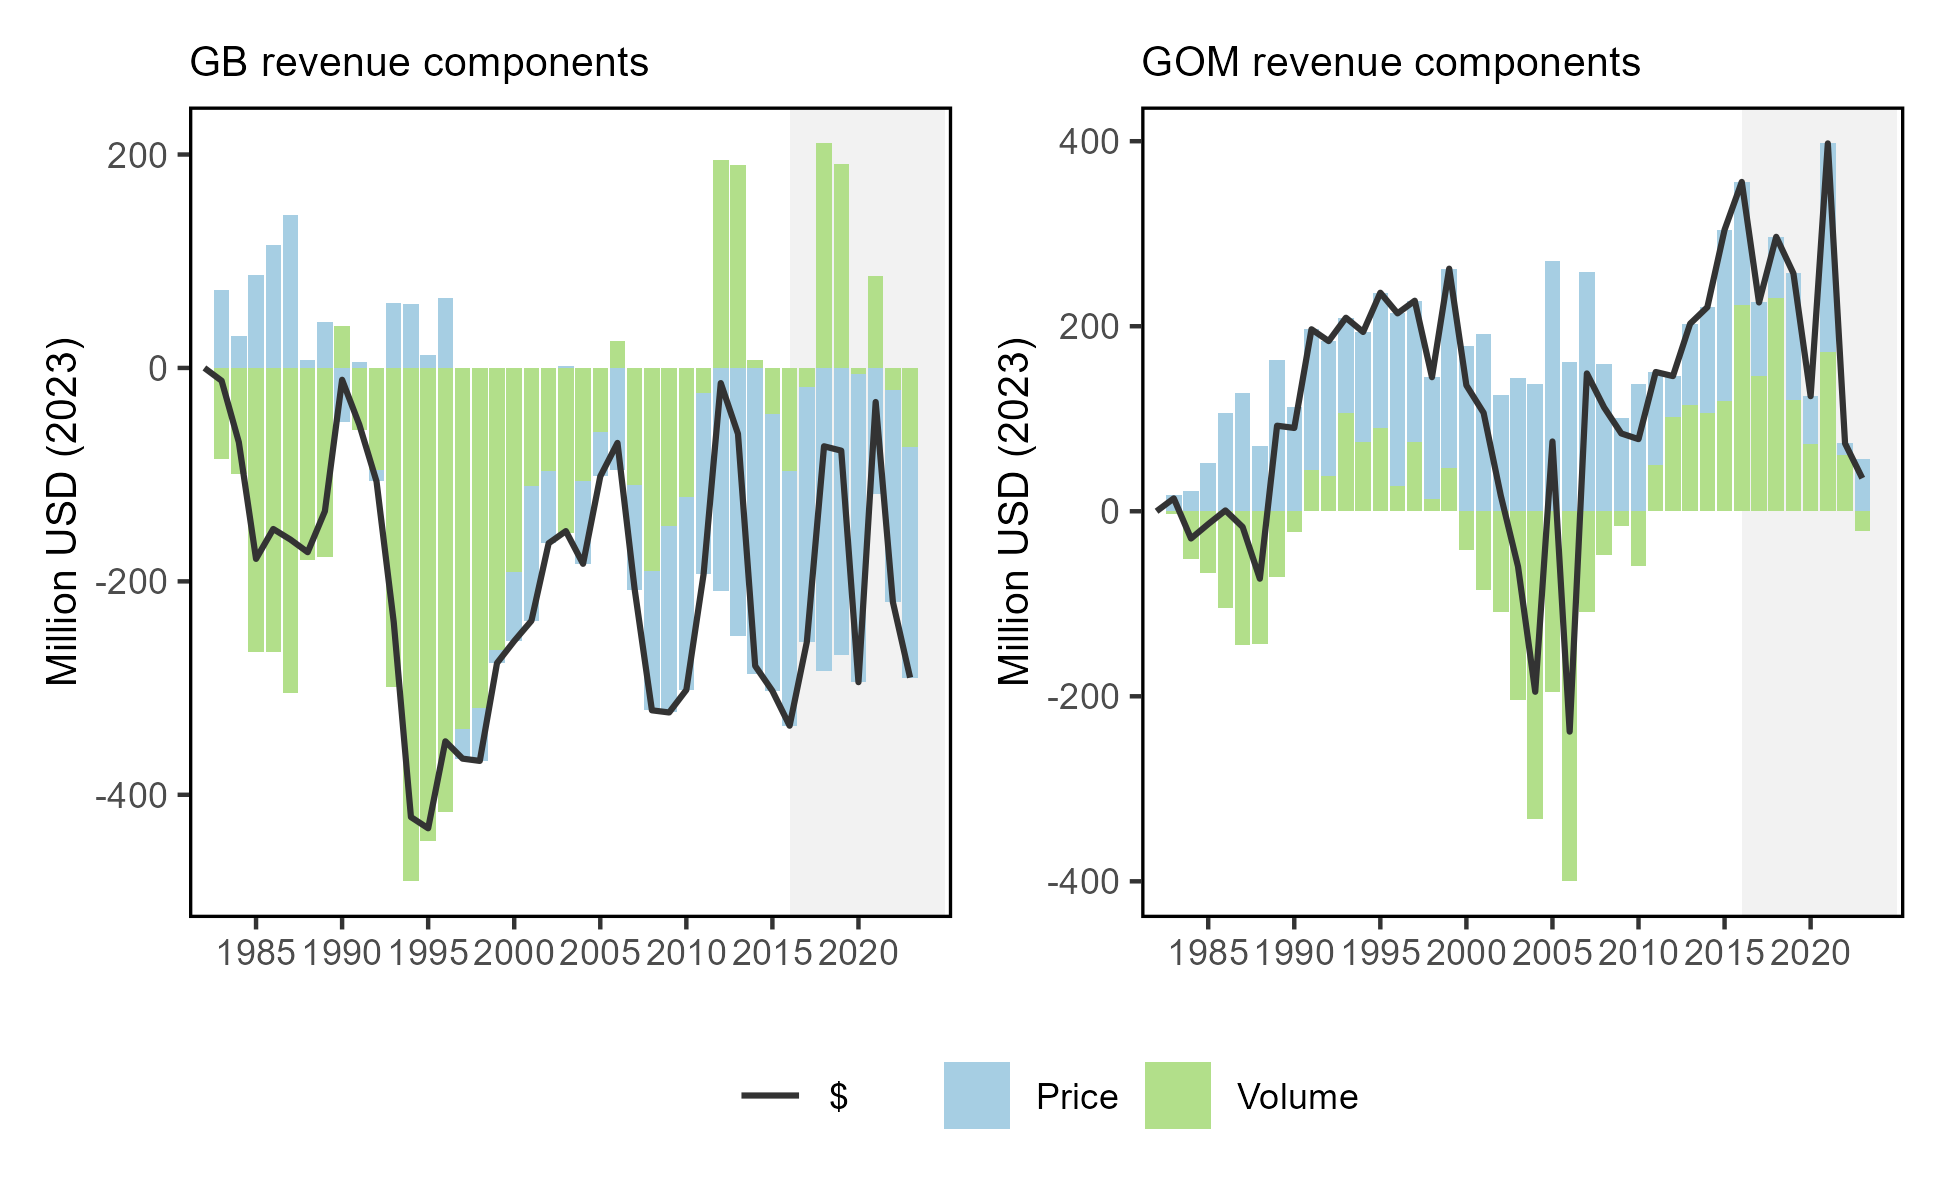
\includegraphics[width=6.5in]{images/NewEngland/bennet_NewEngland_2025-09-09} 

}

\caption{Revenue change from the 1982 baseline in 2023 dollars (black), price, and volume for commercial landings from Georges Bank (GB: left) and the Gulf of Maine (GOM: right)}\label{fig:bennet-82}
\end{figure}

\begin{figure}

{\centering 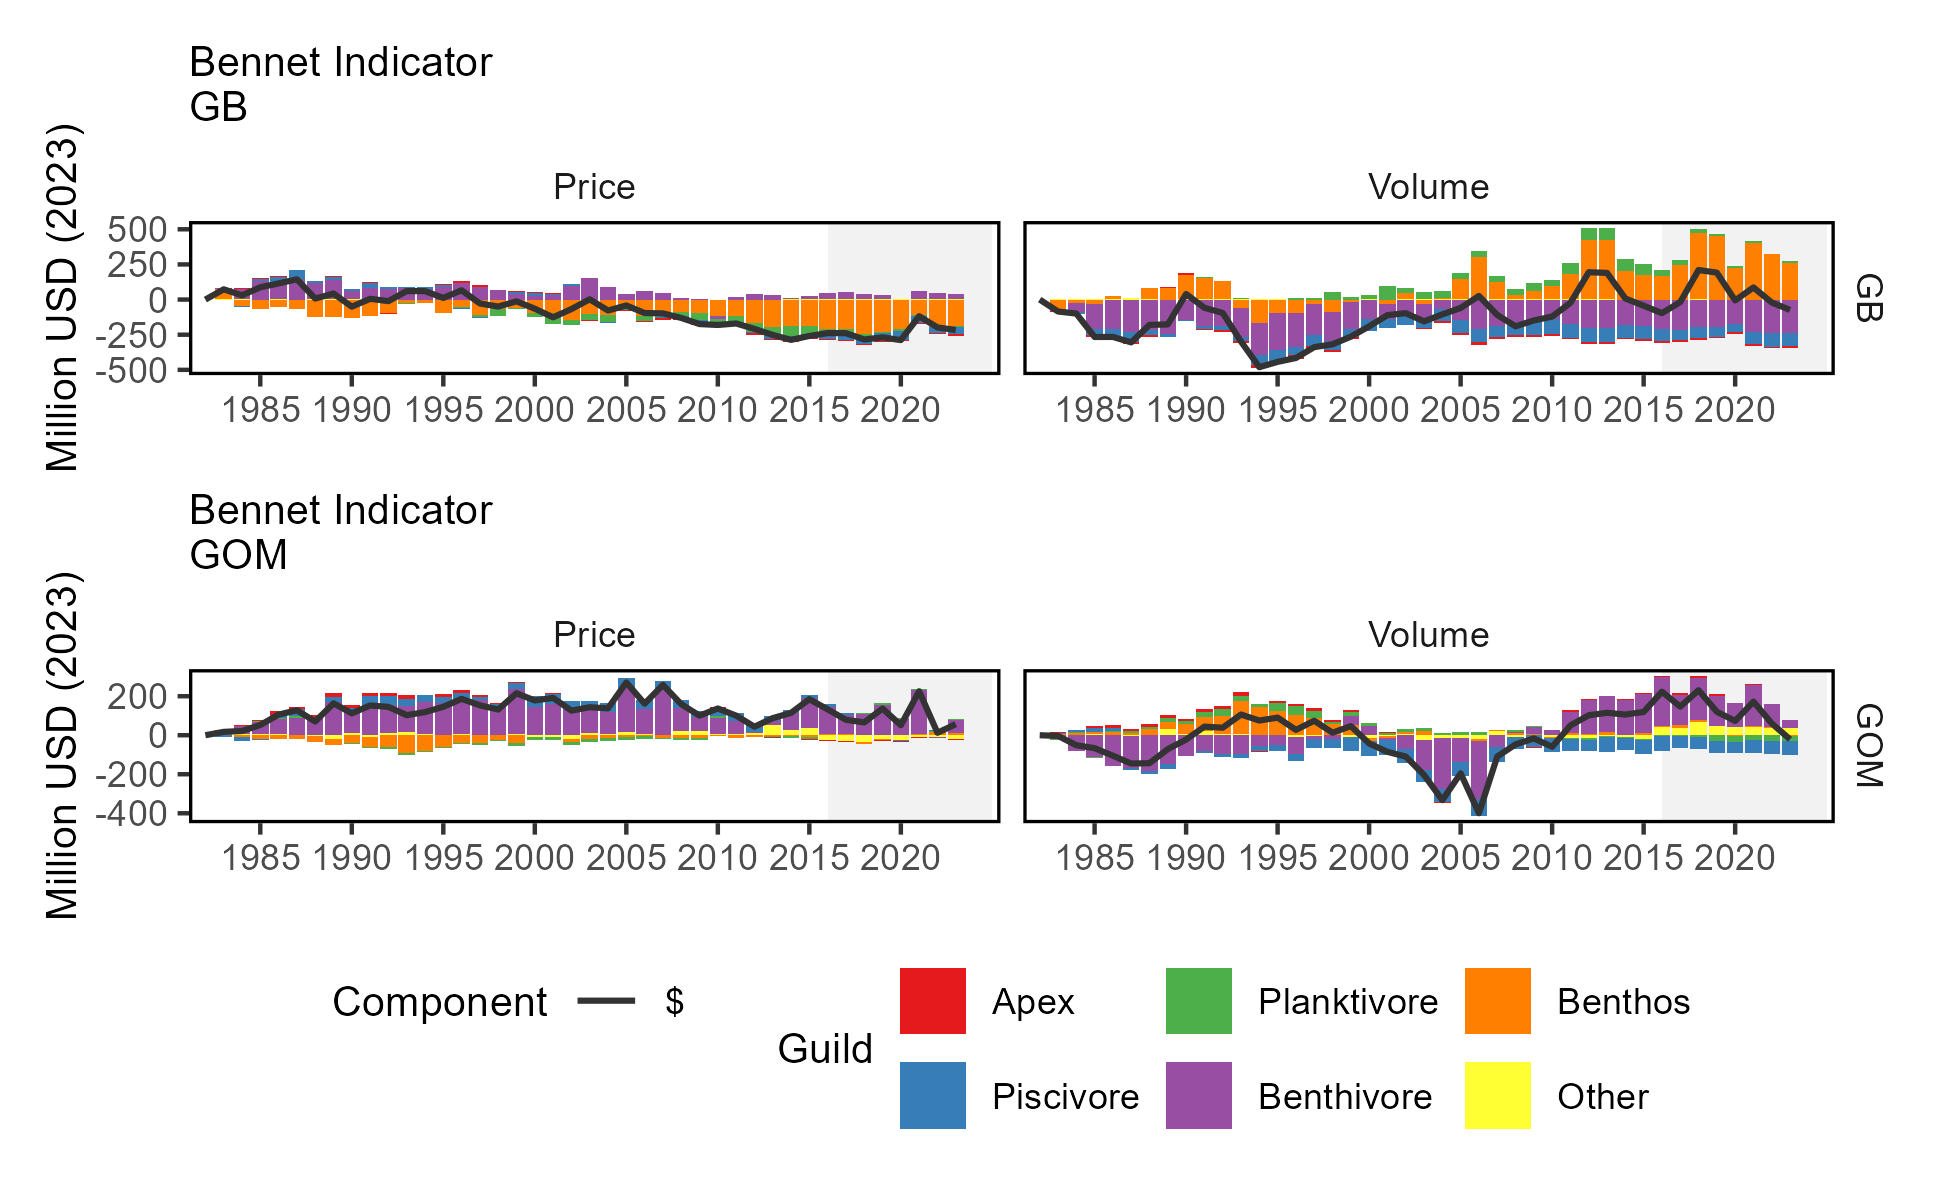
\includegraphics[width=6.5in]{images/NewEngland/bennet_all_NewEngland_2025-09-09} 

}

\caption{Revenue change from the long-term mean in 2023 dollars (black), price, and volume for commercial landings from Georges Bank (GB: top panels) and the Gulf of Maine (GOM: bottom panels)}\label{fig:bennet-all-83}
\end{figure}

For New England, \href{https://noaa-edab.github.io/catalog/community_climate_vulnerability.html}{total climate vulnerability} of revenue was moderate in 2022 with no long-term trend (Fig. \ref{fig:comm-clim-rev}). This suggests that while New England commercial fishing is moderately reliant on climate-sensitive species, this proportion has not significantly changed since 2000.

\begin{figure}

{\centering 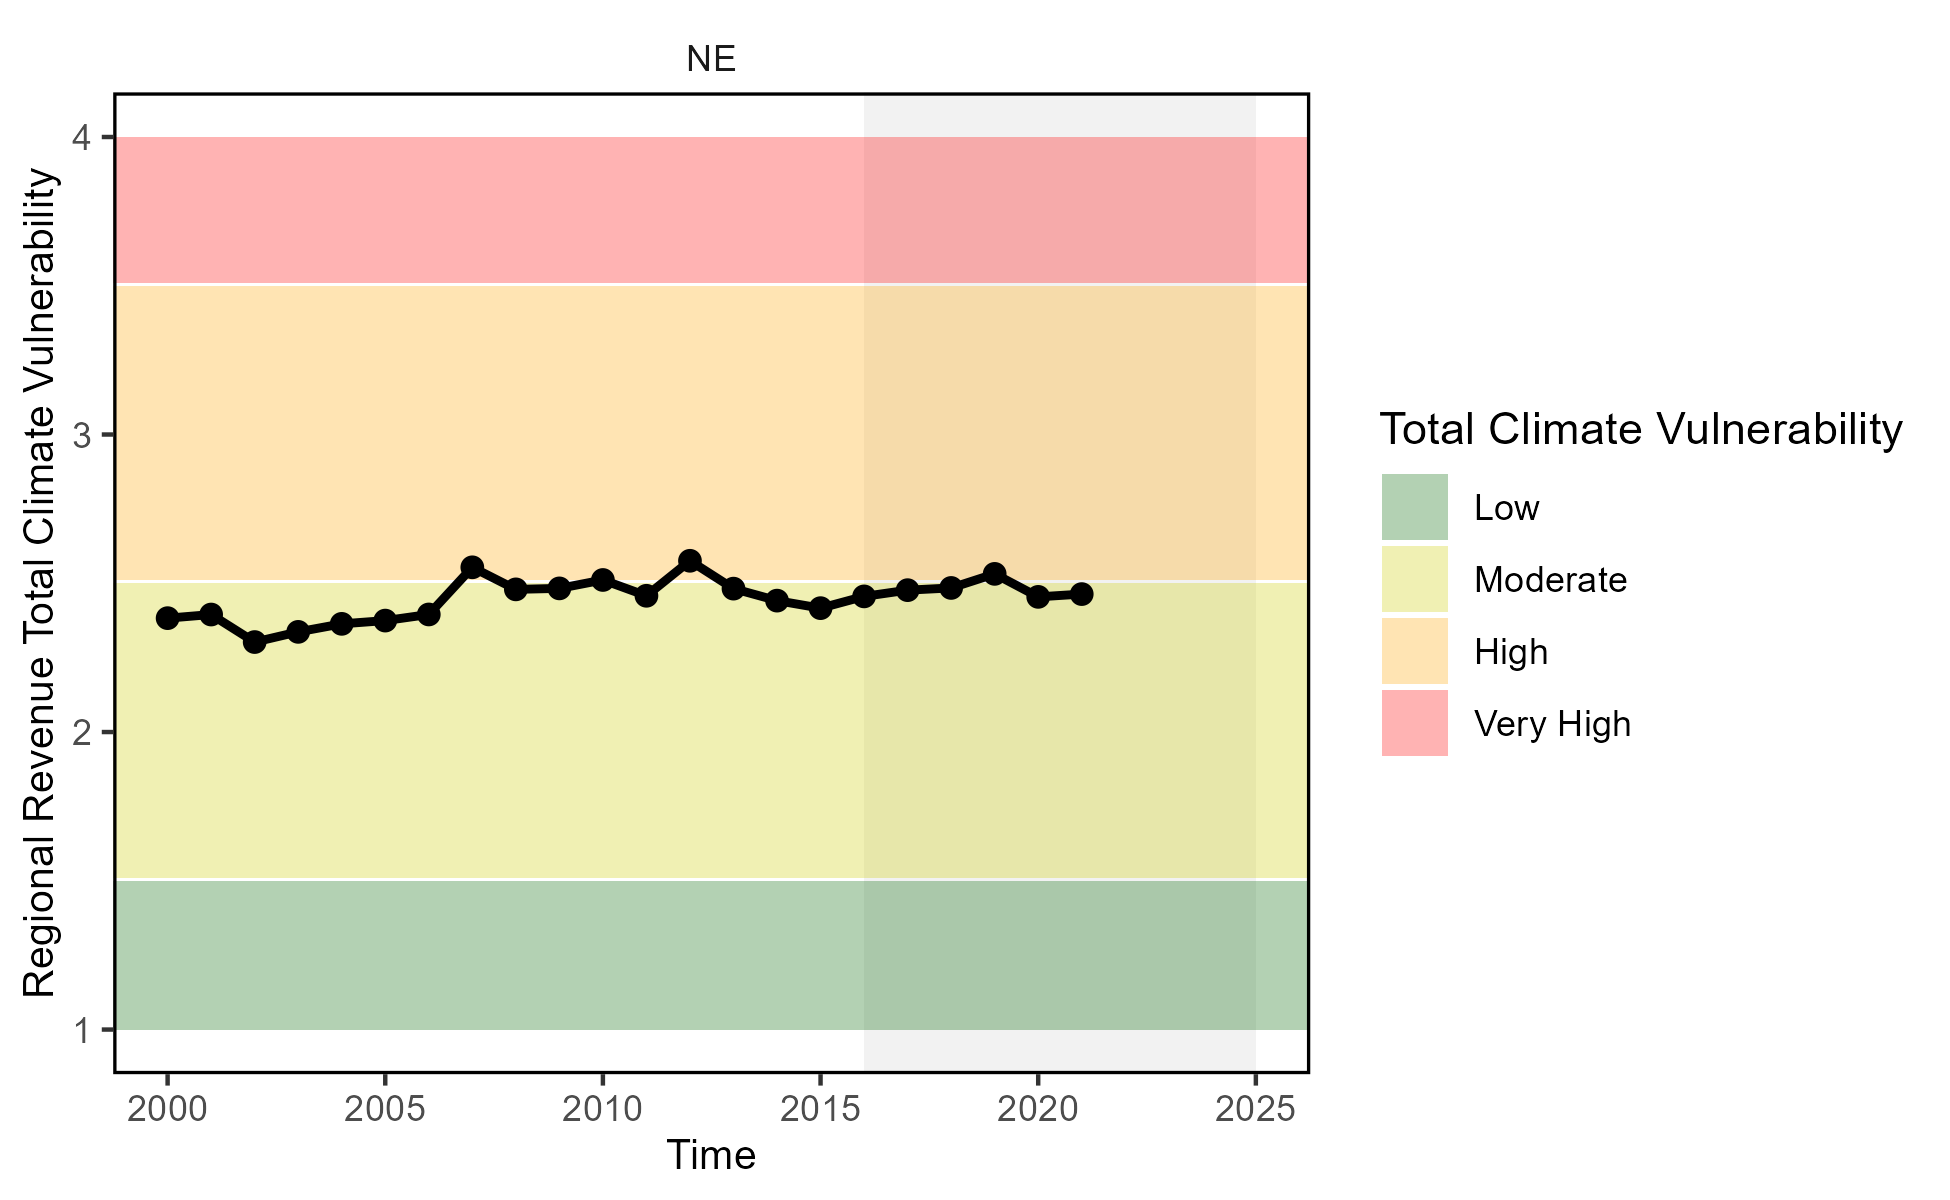
\includegraphics[width=6.5in]{images/NewEngland/climatevul_rev_NewEngland_2025-09-09} 

}

\caption{Total climate vulnerability on New England revenue from 2000 to 2022. Horizontal colored bars show different climate risk levels.}\label{fig:comm-clim-rev}
\end{figure}

\subsubsection{Implications}\label{implications-3}

The continued dependence on lobster in the GOM and sea scallops on GB is affected by multiple drivers including resource availability and market conditions. As both species are sensitive to ocean warming and acidification, it is important to monitor these and other climate drivers.

\section{parent\_report.Rmd}\label{parent_report.rmd-4}

\subsection{Recreational Opportunities}\label{recreational-opportunities}

\end{document}
